\documentclass[a4paper,11pt,twoside,openright]{book}

\usepackage[margin=2cm]{geometry}
\usepackage{lmodern}
\usepackage{parskip}
\usepackage{hyperref}
\usepackage{titlesec}
\usepackage{tikz}
\usetikzlibrary{arrows.meta,positioning}
\usepackage{draftwatermark}
\SetWatermarkText{DRAFT}
\SetWatermarkScale{2}
\SetWatermarkColor[gray]{0.9}
\raggedbottom


\makeatletter
\def\cleardoublepage{%
  \clearpage
  \if@twoside
    \ifodd\c@page
    \else
      \hbox{}
      \thispagestyle{empty} % <-- clé ici
      \newpage
      \if@twocolumn
        \hbox{}
        \newpage
      \fi
    \fi
  \fi
}
\makeatother
\newcommand{\tbc}{\textit{[To be completed...]}}
\newcommand{\TBC}{\begin{center}\textit{To be completed...}\end{center}}

\newcommand{\gpref}[2]{(cf. \cite{#1}, #2)}


% --- APDU Command Diagram Macro ---
% Parameters:
% #1 CLA
% #2 INS
% #3 P1
% #4 P2
% #5 Lc
% #6 Le
% #7 Incoming payload description (or "none")
% #8 Outgoing payload description (or "none")
\newcommand{\apdudesc}[8]{%
\par\medskip
\begingroup
\def\hasin{1}%
\def\hasout{1}%
\ifstrequal{#7}{none}{\def\hasin{0}}{}%
\ifstrequal{#8}{none}{\def\hasout{0}}{}%
% Vertical layout:
% - if there is no incoming payload, command line moves down
% - if there is no outgoing payload, response payload line disappears and SW line moves up
\def\ycmd{0}%
\def\yin{-1}%
\def\yout{-2}%
\def\ysw{-3}%
\ifstrequal{\hasin}{0}{%
  \def\ycmd{-0.5}%
}{}
\ifstrequal{\hasout}{0}{%
  \def\ysw{-2}%
}{}
\begin{center}
\begin{figure}[ht]
\begin{tikzpicture}[
    box/.style={draw, rounded corners, minimum width=1.4cm, minimum height=0.8cm, font=\scriptsize},
    bigbox/.style={draw, rounded corners, minimum width=4cm, minimum height=0.8cm, font=\scriptsize},
    arrow/.style={->, thick}
]
% Client / Secure Element
\node at (-6,1.3) {\textbf{Client}};
\node at (7,1.3) {\textbf{Secure Element}};
% Vertical labels
\node[rotate=90] at (-6.2,\ycmd-0.5) {\textit{APDU}};
\node[rotate=90] at (-6.6,\ycmd-0.5) {\textit{Command}};
\node[rotate=90] at (8.2,\ysw+0.5)  {\textit{APDU}};
\node[rotate=90] at (8.6,\ysw+0.5)  {\textit{Response}};
% Header boxes
\node            at (-3,\ycmd+0.6) {\texttt{CLA}};
\node[box] (cla) at (-3,\ycmd) {\\#1};
\node            at (-1.5,\ycmd+0.6) {\texttt{INS}};
\node[box] (ins) at (-1.5,\ycmd) {\\#2};
\node            at (0,\ycmd+0.6) {\texttt{P1}};
\node[box] (p1)  at (0,\ycmd) {\\#3};
\node            at (1.5,\ycmd+0.6) {\texttt{P2}};
\node[box] (p2)  at (1.5,\ycmd) {\\#4};
\node            at (3,\ycmd+0.6) {\texttt{Lc}};
\node[box] (lc)  at (3,\ycmd) {\\#5};
\node            at (4.5,\ycmd+0.6) {\texttt{Le}};
\node[box] (le)  at (4.5,\ycmd) {\\#6};
% Command header arrows
\draw[arrow] (-6,\ycmd) -- (cla);
\draw[arrow] (le) -- (8,\ycmd);
% Optional incoming payload
\ifstrequal{#7}{none}{%
}{
  \node[bigbox] (in) at (0.75,\yin) {incoming payload of \texttt{Lc} bytes for #7};
  \draw[arrow] (-6,\yin) -- (in);
  \draw[arrow] (in) -- (8,\yin);
}
% Optional outgoing payload
\ifstrequal{#8}{none}{%
}{
  \node[bigbox] (out) at (1,\yout) {outgoing payload of \texttt{Le} bytes for #8};
  \draw[arrow] (8,\yout) -- (out);
  \draw[arrow] (out) -- (-6,\yout);
}
% SW
\node[box] (sw1) at (0,\ysw)       {\texttt{90}};
\node            at (0,\ysw-0.6)   {\texttt{SW1}};
\node[box] (sw2) at (1.5,\ysw)     {\texttt{00}};
\node            at (1.5,\ysw-0.6) {\texttt{SW2}};
\draw[arrow] (8,\ysw) -- (sw2);
\draw[arrow] (sw1) -- (-6,\ysw);
\end{tikzpicture}
\end{figure}
\end{center}
\endgroup
}

\title{oXiDe SE: An Open Source Global Platform Environment Architecture}
\author{}
\date{\today}
\hypersetup{
  pdftitle={oXiDe SE: An Open Source Global Platform Environment Architecture},
  pdfauthor={Gilles Grimaud}
}

\begin{document}

%--------------------------------------------------
\begin{titlepage}
\centering

\vspace*{2cm}

{\Huge \textbf{oXiDe SE} \par}

\vspace{0.5cm}

{\Large An Open Source Global Platform Environment Architecture \par}

\vspace{1.5cm}

{\Large Gilles Grimaud$^{1,2,3}$ \par}

\vspace{0.5cm}

\small
$^{1}$ Univ. Lille, UMR 9189 CRIStAL, F-59000 Lille, France\\
$^{2}$ CNRS, UMR 9189, F-59000 Lille, France\\
$^{3}$ Centrale Lille, F-59000 Lille, France

\vspace{1cm}

{\large Université de Lille}

\vspace{1cm}

{\large \today}

\vfill

\end{titlepage}

\tableofcontents
\newpage

% --------------------------------------------------
% Principaux TODO suite a une relecture en profondeur au 05/04/26
%
% 1. Les sous-sections d'implementation reellement necessaires au developpement
%    sont encore absentes. En pratique, LOAD, INSTALL, DELETE, le registre, les
%    Security Domains, SCP03, les canaux logiques et la gestion fine des etats
%    n'ont pas encore de description exploitable.
%
% 2. La frontiere de services privilegies entre le kernel et les applications
%    administratives reste conceptuelle. L'idee est bien expliquee, mais pas le
%    contrat. Il manque la forme concrete de l'API noyau : operations offertes,
%    parametres, representation des privileges, regles de validation, modele
%    d'erreur, propriete des buffers, et lien avec la session securisee.
%
% 3. Le modele d'isolation est clair comme objectif, mais pas encore comme
%    mecanisme. Le document decrit correctement les frontieres
%    kernel / admin apps / ordinary apps, mais ne dit pas comment elles sont
%    imposees : separation memoire, handles, capabilities, mediation sur objets
%    persistants, appels inter-applications, partage controle, ou strategie
%    d'execution concrete. Pour un ingenieur, c'est encore un modele de
%    securite, pas une architecture executable.
%
% 4. Le cycle de vie est encore trop narratif. Il manque des tables ou
%    automates explicites par type d'objet : Executable Load File, application
%    instance, Security Domain, avec etats permis, transitions legales,
%    preconditions et causes de rejet.
%
% 5. La cartographie "qui traite quelle commande GP" n'est pas encore assez
%    explicite pour implementer le dispatch. Le document dit bien que SELECT
%    est preemptif et que le reste va a l'application selectionnee, mais il
%    manque une matrice claire par commande : OPEN-level, commande SD, commande
%    applicative, commande transport, contexte requis, privileges requis.
%
% 6. Les contraintes temporelles T=0 sont bien motivees, mais pas encore
%    transformees en exigences d'implementation verifiables. Il manque des
%    budgets concrets par cible, les hypotheses d'horloge/UART/interruptions,
%    et surtout la methode de validation : comment on mesure, quelle marge on
%    vise, et comment on evite une regression.
%
% 7. Le debut du document n'est pas totalement aligne avec la structure
%    actuelle. L'Architecture Overview presente encore quatre "major
%    components" comme des blocs homogenes, alors que le corps du manuel
%    distingue maintenant beaucoup plus nettement : modele GP, lecture systeme,
%    puis implementation. Ce n'est pas faux, mais c'est moins net que le reste.
%
% 8. Le chapitre d'implementation contient encore un marqueur non credible
%     pour un lecteur externe. L'URL associee a la reference implementation
%     pointe encore vers un depot fictif, ce qui cree une friction inutile pour
%     un ingenieur qui veut suivre la documentation avec le code.
%
%--------------------------------------------------

\chapter{Architecture Overview}

This document studies \textbf{oXiDe SE}, a concrete open source secure-element
operating system and its reference implementation. The architecture presented
here is therefore not only a generic interpretation of GlobalPlatform: it is
the security and software architecture against which the oXiDe SE source tree,
build configurations, and validation results are to be evaluated. Where the
document generalizes from the implementation, it does so explicitly in order to
identify design principles that may be reused by other open secure-element
systems.

oXiDe SE is designed to run under QEMU in order to make development, testing,
and external contributions easier, but its intended deployment targets are
real, readily available microcontrollers. The current ports cover the Arm
Cortex-M architecture profiles Armv6-M, Armv7-M, and Armv8-M. The primary
targets are \texttt{mps2-an385}, \texttt{raspi-pico1}, and
\texttt{raspi-pico2}: the first two can be exercised under QEMU, while the two
Raspberry Pi Pico generations are also validated on widely available physical
boards.

The architecture is also intended to support deployment in the Arm TrustZone
secure world on processors that provide it. In this configuration, oXiDe SE
would expose secure-element services from an isolated execution environment and
act as a \emph{virtual Secure Element} for software running outside that trusted
world.

%--------------------------------------------------
\section{oXiDe SE Architectural Contribution}

GlobalPlatform defines an external management model, its managed entities, and
the protocols used to administer them. It does not prescribe one unique
internal operating-system decomposition. The architectural contribution of
oXiDe SE lies in the way it maps that model onto a small Rust-based embedded
system:

\begin{itemize}
\item a deliberately narrow kernel owns platform-global control flow,
  selection, APDU mediation, isolation, and the structural invariants of the
  persistent registry;
\item Security Domains are first-class administrative application-like objects
  rather than labels or a collection of unrelated special cases embedded
  throughout the kernel;
\item a Security Domain supplies authority, policy, and secure-channel context,
  while the kernel retains validation, non-escalation checks, and final
  mediation of privileged effects;
\item ordinary applications, called \emph{Rustlets}, are independently built
  FAE images executed behind a narrow ABI and a privileged-service boundary.
  They are generally intended for post-issuance deployment, although oXiDe SE
  also permits Rustlets to be embedded in an image before issuance. These two
  positions relative to issuance are shown in
  Figure~\ref{fig:se-lifecycle-actors} and explained further in
  Section~\ref{sec:gp-deployment-workflow};
\item target-specific hardware support and development backends are kept below
  the same APDU and application model, while their distinct security properties
  remain explicit.
\end{itemize}

The central architectural proposition is not merely that GlobalPlatform
commands can be implemented in Rust. It is that GlobalPlatform administration can be decomposed
between a small invariant-enforcing kernel and bounded administrative
applications without giving ordinary applications direct access to
platform-global state. This separation is intended to make authority,
isolation, persistence, and command dispatch independently analyzable.

%--------------------------------------------------
\section{Trusted Computing Base}

For this manual, the trusted computing base (TCB) comprises the components whose
correctness is required to support the security properties sought for an
oXiDe SE image. Its exact hardware portion depends on the selected target, but
its software portion includes:

\begin{itemize}
\item the trusted boot and execution substrate, including the target support
  used for exception handling, memory protection, interrupts, transport,
  persistent flash, cryptographic primitives, and entropy acquisition;
\item the kernel code that parses and mediates APDUs, maintains the selected
  context, enforces isolation, validates privileged requests, owns the registry,
  and commits persistent mutations;
\item every privileged component statically linked into the kernel image,
  including any build-selected kernel-resident module;
\item the root Security Domain and each administrative Security Domain, but only
  for the policy and authority entrusted to that domain. A Rustlet-backed
  Security Domain remains isolated by the kernel, yet its authorization logic
  is part of the policy TCB for its own administrative subtree;
\item the configured trust anchors, privilege assignments, and build-time
  security configuration that determine which authorities the resulting image
  accepts.
\end{itemize}

Ordinary Rustlets are explicitly outside the TCB and must be treated as
potentially malicious. They may affect their own state and obtain only effects
granted through mediated services. A compromised supplementary Security Domain
may misuse its delegated authority, but the kernel is expected to prevent that
authority from escaping its assigned subtree or bypassing platform invariants.

The compiler, image-construction tools, provisioning process, and hardware
supply chain are necessary trust assumptions for producing the initial trusted
image, but they are not resident components of the runtime TCB. QEMU, host-side
test programs, and semihosting services are likewise outside that runtime TCB.
Chapter~2 states the corresponding attacker model, assumptions, and exclusions.

%--------------------------------------------------
\section{How The Architecture Is Assessed In This Manual}

This overview introduces design objectives; it does not present them as
formally established guarantees. The remainder of the manual progressively
describes the mechanisms, intended properties, assumptions, known limits, and
available validation evidence against which oXiDe SE can be assessed:

\begin{itemize}
\item Chapter~2 defines the assets, adversaries, trust assumptions, security
  goals, and explicitly out-of-scope attacks;
\item Chapter~3 defines the APDU, command-dispatch, and secure-channel protocol
  contracts at the external boundary;
\item Chapter~4 defines the managed-object, lifecycle, deployment, and
  administrative-authority invariants inherited from the GlobalPlatform model;
\item Chapter~5 identifies the internal decomposition, kernel responsibilities,
  privileged-service boundary, Security Domain authority, and isolation model;
\item Chapter~6 defines registry persistence and the transactional behavior
  required across interrupted flash updates and resets;
\item Chapter~7 defines the Rustlet execution and ABI model, including the
  application-facing boundary and its isolation requirements;
\item Chapter~8 maps those abstractions to the reference implementation and
  records the present implementation scope and limitations;
\item the appendices refine the T=0 and secure-channel encodings and document
  the provenance and limits of the regression material used for validation.
\end{itemize}

The companion abstract model in \texttt{docs/model.md} collects the principal
state invariants and reasoning obligations in a lightweight Hoare-style
notation. These obligations have not yet been discharged through a complete
formal verification. The source code and executable tests provide implementation
and regression evidence, not a formal proof or a security certification.
Likewise, passing under QEMU does not establish security on physical hardware.

%--------------------------------------------------
\section{Secure Element Ecosystem and Lifecycle}

Before introducing the technical decomposition of the platform, it is useful to
place the secure element in its operational ecosystem. A secure element does
not exist in isolation: it changes hands several times during its life, and
different actors contribute different layers of hardware, software,
configuration and deployed services.

For the purpose of this manual, the surrounding ecosystem is organized around
five actor categories.

\begin{itemize}
\item \textbf{Foundries} manufacture the silicon and deliver the physical secure
  element as a hardware component.
\item \textbf{Providers} integrate the hardware into a usable platform,
  implement the base software stack, and package the secure element together
  with its kernel and foundational services.
\item \textbf{Issuers} distribute the resulting device or object and control its
  initial personalization, provisioning and operational enrollment.
\item \textbf{Service providers} deploy service-specific applications and data,
  either during manufacturing, under agreement with the issuer, or later in the
  field through post-issuance channels such as OTA updates.
\item \textbf{End users} operate the final device and consume the services
  exposed through the secure element, often without directly perceiving the
  existence of the secure element itself.
\end{itemize}

These actors intervene at different moments of the secure-element lifecycle and
do not all manipulate the same interfaces. Foundries first create the physical
substrate. Providers then transform that substrate into a secure-element
platform by activating the hardware, deploying the kernel and installing the
base software that will later anchor the root of trust. Issuers receive that
platform and personalize it for a product line or deployment context. Service
providers add dedicated applications and associated secrets. End users finally
interact with the resulting device through its exposed services and external
communication channels.

\begin{figure}[ht]
  \centering
  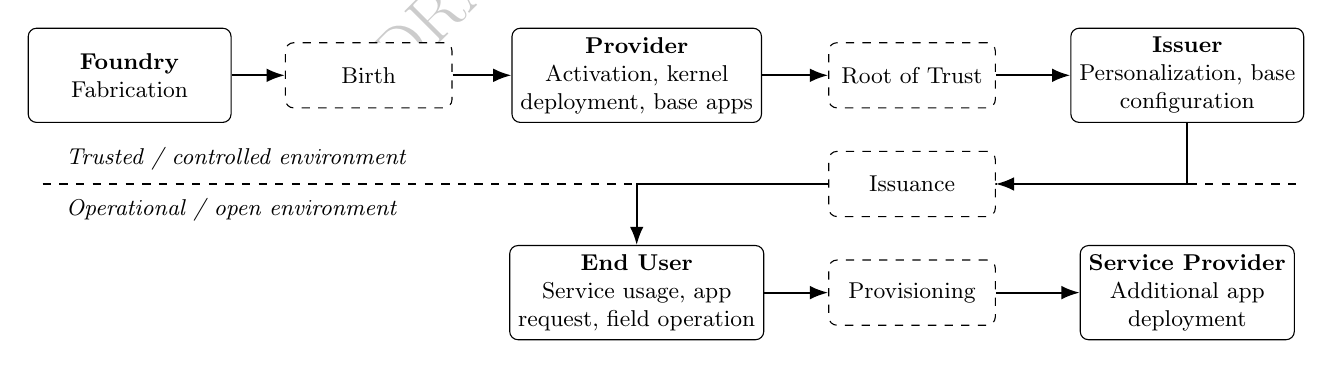
\begin{tikzpicture}[
    scale=0.92,
    transform shape,
    stage/.style={
      draw,
      rounded corners=3pt,
      minimum width=2.8cm,
      minimum height=1.3cm,
      align=center,
      font=\small
    },
    state/.style={
      draw,
      dashed,
      rounded corners=3pt,
      minimum width=2.3cm,
      minimum height=0.9cm,
      align=center,
      font=\small,
      fill=white,
      inner sep=3pt
    },
    zone/.style={
      font=\small\itshape
    },
    >=Latex
  ]

    % --- Top line
    \node[stage] (foundry) at (0,0) {\textbf{Foundry}\\Fabrication};
    \node[state] (birth) at (3.3,0) {Birth};
    \node[stage] (provider) at (7.0,0) {\textbf{Provider}\\Activation, kernel\\deployment, base apps};
    \node[state] (rot) at (10.8,0) {Root of Trust};
    \node[stage] (issuer) at (14.6,0) {\textbf{Issuer}\\Personalization, base\\configuration};

    % --- Bottom line (recentered)
    \node[stage] (user) at (7.0,-3.0) {\textbf{End User}\\Service usage, app\\request, field operation};
    \node[state] (prov) at (10.8,-3.0) {Provisioning};
    \node[stage] (sp) at (14.6,-3.0) {\textbf{Service Provider}\\Additional app\\deployment};

    % --- Top flow 
    \draw[->, thick] (foundry.east) -- (birth.west);
    \draw[->, thick] (birth.east) -- (provider.west);
    \draw[->, thick] (provider.east) -- (rot.west);
    \draw[->, thick] (rot.east) -- (issuer.west);

    % --- Separation line (drawn first so nodes can mask it) 
    \draw[dashed, thick] (-1.2,-1.5) -- (16.2,-1.5);

    % --- Zone labels
    \node[zone, anchor=west] at (-1.0,-1.15) {Trusted / controlled environment};
    \node[zone, anchor=west] at (-1.0,-1.85) {Operational / open environment};

    % --- Issuance node (positionné entre les deux)
    \node[state] (issuance) at (10.8,-1.5) {Issuance};

    % --- Arrow 1: Issuer -> Issuance (descend puis gauche)
    \draw[->, thick]
      (issuer.south) -- ++(0,-0.8) |- (issuance.east);

    % --- Arrow 2: Issuance -> End User (gauche puis descend)
    \draw[->, thick]
      (issuance.west) -| (user.north);

    % --- Provisioning flow
    \draw[->, thick] (user.east) -- (prov.west);
    \draw[->, thick] (prov.east) -- (sp.west);

  \end{tikzpicture}
  \caption{Simplified lifecycle of a secure element and transfer of responsibility between actors.}
  \label{fig:se-lifecycle-actors}
\end{figure}

Figure~\ref{fig:se-lifecycle-actors} should not be read as a rigid industrial
workflow. In practice, a single organization may play several roles, and some
deployment steps may occur earlier or later depending on the business model.
The important point for the rest of this manual is that the same secure element
progressively accumulates hardware properties, kernel-level trust anchors,
issuer-specific configuration and service-provider payloads before being used
in the field.

The architecture is structured into four major components.

%--------------------------------------------------
\section{Communication and Protocol}

This component is responsible for handling all interactions between the
external world and the platform. It defines how commands are transported,
interpreted and secured. It is the entry point through which incoming requests
must pass for decoding and validation before execution;
the effectiveness of those checks is assessed in the later protocol and
implementation chapters.

\begin{itemize}
\item \textbf{APDU transport layer} \gpref{gp-card}{§5.3, §9.4}
\item \textbf{APDU parser and dispatcher} \gpref{gp-card}{§9.4, §11}
\item \textbf{Secure Channel Protocol (SCP)} \gpref{scp03}{§4, §6, §7}
\end{itemize}

The APDU transport layer corresponds to the low-level communication defined in
ISO/IEC 7816 and referenced in the GlobalPlatform card specification. Sections
§5.3 and §9.4 describe how commands are encapsulated and exchanged. This layer
is responsible for transporting APDUs across the selected physical or emulated
medium while preserving the command representation expected by the parser.

The APDU parser and dispatcher implements the command interpretation logic
described in §9.4 and §11. It decodes the APDU structure and maps each command
(such as INSTALL, LOAD, DELETE) to its corresponding internal handler. This
component effectively bridges the external protocol with the internal execution
model.

The Secure Channel Protocol, described in SCP03 (§4, §6, §7), introduces
cryptographic protection over APDU exchanges. It defines how sessions are
established, how keys are derived, and how messages are authenticated and
optionally encrypted. The protocol is intended to provide integrity and
confidentiality for administrative commands when it is correctly configured,
implemented, and used within its stated assumptions.

%--------------------------------------------------
\section{GlobalPlatform Conceptual Model}

This component introduces the main conceptual entities manipulated by a
GlobalPlatform secure element. It describes what kinds of objects exist on the
secure element, how they relate to each other, how their lifecycle is controlled,
and how administration authority is represented. It remains at the level
of GlobalPlatform concepts rather than of internal software
decomposition.

\begin{itemize}
\item \textbf{Managed objects}: load files, application instances, and Security
  Domains \gpref{gp-card}{§7, §9}
\item \textbf{AID-based identification and relationships}
  \gpref{gp-card}{§6.2, §7}
\item \textbf{Lifecycle states and transitions}
  \gpref{gp-card}{§9.6}
\item \textbf{Deployment and personalization workflows}
  \gpref{gp-card}{§9, §11}
\item \textbf{Administrative authority and privileges}
  \gpref{gp-card}{§7, §11.1.2}
\end{itemize}

This conceptual layer explains, for instance, why a load file, an
installed application instance, and a Security Domain are distinct
entities even when they are operationally related.

It also explains why commands such as \texttt{LOAD}, \texttt{INSTALL},
\texttt{DELETE}, \texttt{PUT KEY}, or \texttt{SET STATUS} should be read
against a shared administration model rather than as isolated APDU
opcodes.

The implementation-specific mapping of those concepts onto a kernel and
resident applications is deferred to the later execution-model chapter.

%--------------------------------------------------
\section{Model, Security and Core Services}

This component defines the internal structure of the platform. It is
responsible for maintaining consistency, enforcing isolation and providing the
cryptographic foundation required for secure operations.

\begin{itemize}
\item \textbf{Registry of managed objects} \gpref{gp-card}{§9.3}
\item \textbf{AID management} \gpref{gp-card}{§6.2, §9.3.1}
\item \textbf{Secure persistence} \gpref{gp-card}{§9}
\item \textbf{Security Domains} \gpref{gp-card}{§7}
\item \textbf{Privilege and access control} \gpref{gp-card}{§11.1.2}
\item \textbf{Key management} \gpref{scp03}{§6.2, §6.3}
\item \textbf{Cryptographic services} \gpref{scp03}{§6}
\item \textbf{Logging and audit} \gpref{gp-card}{§9}
\end{itemize}

The registry, described in §9.3, maintains the internal representation of all
entities managed by the platform. It is the authoritative source of truth for
application instances, load files and Security Domains.

AID management, defined in §6.2 and §9.3.1, is intended to maintain unique
identification of all entities. It also supports selection mechanisms used by
APDU commands.

Secure persistence is intended to keep the registry and associated metadata
transactionally consistent across resets. The concrete mechanism, failure
model, and current validation evidence are described later in this manual.

Security Domains (§7) define administrative boundaries. They allow grouping
applications under a shared authority and delegating management capabilities.

Privileges and access control (§11.1.2) define what operations an application
or domain can perform. These include administrative rights such as loading or
deleting applications.

Key management and cryptographic services are defined in SCP03 (§6). They
specify how keys are stored, derived and used for secure communication.

Logging and audit mechanisms provide traceability of operations and support
debugging and security analysis.

%--------------------------------------------------
\section{System Decomposition and Execution Model}

This component describes the internal software architecture chosen by the
project to realize the GlobalPlatform concepts introduced above. It is
explicitly an implementation reading of the specification rather than a
normative statement about how every GlobalPlatform secure element must be built.

\begin{itemize}
\item \textbf{A small kernel handling platform-global control flow}
\item \textbf{Administrative applications}, notably Security Domains
\item \textbf{Ordinary applications selected and invoked through APDUs}
\item \textbf{A privileged service boundary} between applications and
  kernel-managed effects
\end{itemize}

The resulting model keeps \texttt{SELECT} and other context-defining
operations in the kernel while routing most other APDUs to the currently
selected AID-associated entity.

In that decomposition, Security Domains are realized as privileged
administrative applications rather than as ad hoc kernel branches for
every management command. This keeps APDU dispatch uniform while still
preserving a strict authority boundary for sensitive operations.

%--------------------------------------------------

\section{Layered Architecture}

The architecture introduced in the previous sections can be summarized as a
layered stack. 

\begin{figure}[ht]
  \centering
  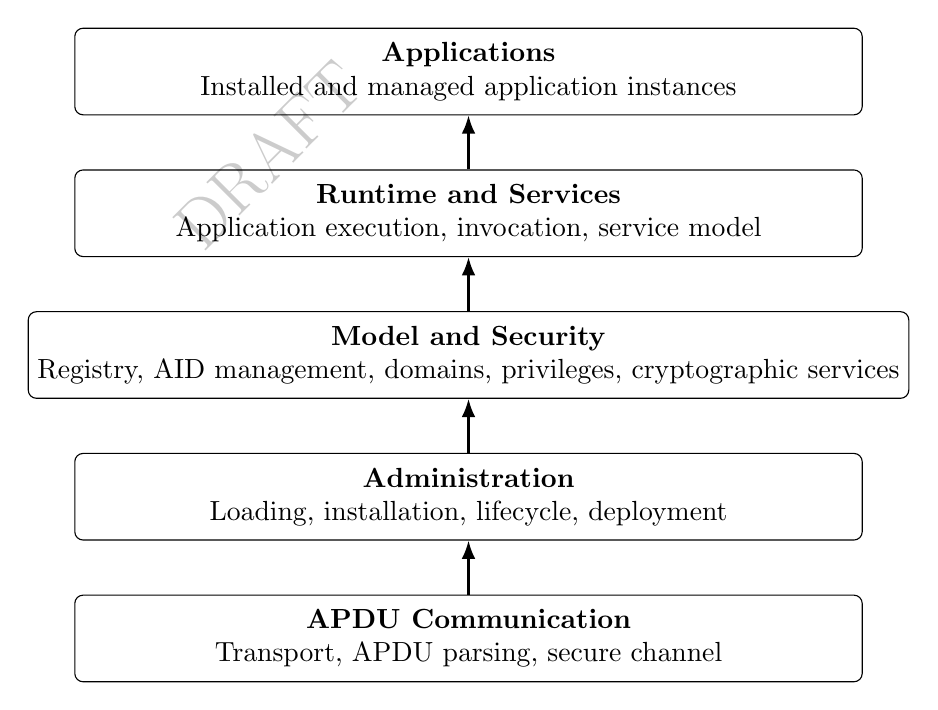
\begin{tikzpicture}[
    layer/.style={
      draw,
      rounded corners=3pt,
      minimum width=10cm,
      minimum height=1.1cm,
      align=center
    },
    >=Latex
  ]
    \node[layer] (apdu) at (0,0)    {\textbf{APDU Communication}\\Transport, APDU parsing, secure channel};
    \node[layer] (admin) at (0,1.8) {\textbf{Administration}\\Loading, installation, lifecycle, deployment};
    \node[layer] (model) at (0,3.6) {\textbf{Model and Security}\\Registry, AID management, domains, privileges, cryptographic services};
    \node[layer] (runtime) at (0,5.4) {\textbf{Runtime and Services}\\Application execution, invocation, service model};
    \node[layer] (apps) at (0,7.2)  {\textbf{Applications}\\Installed and managed application instances};

    \draw[->, thick] (apdu.north) -- (admin.south);
    \draw[->, thick] (admin.north) -- (model.south);
    \draw[->, thick] (model.north) -- (runtime.south);
    \draw[->, thick] (runtime.north) -- (apps.south);
  \end{tikzpicture}
  \caption{Layered view of an open source GlobalPlatform environment architecture.}
  \label{fig:gp-layered-architecture}
\end{figure}

This representation emphasizes the separation of concerns between
communication, administration, internal security mechanisms and application
execution. It also makes explicit the direction of dependency: upper layers
rely on the services provided by lower layers, while lower layers remain
agnostic to the internal logic of upper layers.

Figure~\ref{fig:gp-layered-architecture} highlights the main architectural
principle of the platform. The bottom layer handles communication concerns and
provides a normalized command entry point through APDU processing and secure
messaging. On top of it, the administration layer implements the management
logic required to deploy and control applications. The model and security layer
provides the persistent representation of managed entities together with the
mechanisms that enforce isolation and authorization. Finally, the runtime layer
hosts the execution model exposed to applications. This organization reflects
the fact that GlobalPlatform strongly structures the lower and middle parts of
the stack, while leaving more freedom to the implementation of the execution
environment itself.

%--------------------------------------------------
\section{Glossary}

Unless stated otherwise, the technical vocabulary of this document follows
ISO/IEC~7816 for transport-level concepts and the GlobalPlatform Card
Specification for secure-element-management concepts \gpref{iso7816-4}{§5, §6}
\gpref{gp-card}{§1.4, §6.5, §7}. The purpose of the present glossary is
twofold:
\begin{itemize}
\item to define the technical terms used throughout the document;
\item to keep the text \textbf{secure-element centric}, even though a large
  part of the normative literature remains historically \textbf{card}
  centric.
\end{itemize}

In other words, this document prefers \textbf{secure element} as the generic
system concept, while still acknowledging that ISO/IEC~7816 and
GlobalPlatform often use the word \textbf{card} for the emblematic and
historically dominant form of such a device.

\begin{itemize}
\item \textbf{secure element}: the preferred generic term for the protected
  computing device targeted by this document. It designates the platform that
  stores keys, hosts managed applications, executes APDU commands, and enforces
  the relevant isolation and lifecycle policies.
\item \textbf{card}: the historical and normative term used throughout
  ISO/IEC~7816 and the GlobalPlatform Card Specification for an emblematic
  class of secure element. In this manual, it is retained when the wording of
  the standards is being discussed directly, or when using fixed protocol terms
  such as \emph{card challenge}, \emph{card cryptogram}, or \emph{card
  management command}.
\item \textbf{off-card entity}: the preferred GlobalPlatform term for the
  external party interacting with the secure element.
\item \textbf{interface device}: the ISO/IEC~7816 transport-level term for the
  equipment that exchanges APDUs with the secure element.
\item \textbf{host}: the preferred SCP03 term for the external peer in secure
  channel establishment, notably in \emph{host challenge} and \emph{host
  cryptogram}.
\item \textbf{command APDU}: an APDU sent from the interface device or
  off-card entity to the secure element.
\item \textbf{response APDU}: an APDU returned by the secure element to the
  interface device or off-card entity.
\item \textbf{header}: the four command bytes \texttt{CLA}, \texttt{INS},
  \texttt{P1}, and \texttt{P2}.
\item \textbf{incoming data}: the command payload transported from the
  interface device to the secure element and logically measured by
  \texttt{Lc}.
\item \textbf{outgoing data}: the response payload returned by the secure
  element before the final status word and logically measured by \texttt{Le}.
\item \textbf{status word}: the two-byte trailer \texttt{SW1/SW2} appended to
  a response APDU.
\item \textbf{ATR}: the \emph{Answer To Reset}, i.e. the first byte string
  emitted by the secure element after activation/reset and before the APDU
  command stream begins.
\item \textbf{\texttt{T=0} transport}: the half-duplex, character-oriented
  transport defined by ISO/IEC~7816-3.
\item \textbf{deferred response}: the \texttt{T=0} realization of a logical
  Case~4 exchange, where response data is first announced by \texttt{61xx} and
  then recovered through one or more \texttt{GET RESPONSE} commands.
\item \textbf{application instance}: the preferred term for the installed
  application object managed by the secure element and later selected through
  its AID.
\item \textbf{ordinary application}: a non-administrative application instance
  implementing business logic rather than GlobalPlatform administration.
\item \textbf{administrative application}: an application-level component that
  implements administrative semantics and is granted privileged access to
  kernel-mediated services. In the present architecture, Security Domains are
  realized in this category.
\item \textbf{Security Domain}: the GlobalPlatform administrative principal
  associated with keys, privileges, and management authority.
\item \textbf{Issuer Security Domain}: the distinguished Security Domain that
  anchors the main administrative authority of the secure element.
\item \textbf{Card Manager}: a broader historical label often associated in
  practice with the Issuer Security Domain or with its operational role. This
  document keeps \emph{Issuer Security Domain} as the more precise preferred
  term.
\item \textbf{Executable Load File}: the deployable executable content object
  transported through \texttt{LOAD}. After first introduction, this manual uses
  the shorter form \textbf{load file}.
\item \textbf{GlobalPlatform Registry}: the authoritative catalogue of managed
  objects, identities, privileges, lifecycle states, and dependencies within
  the secure element. After first introduction, this manual uses the shorter
  form \textbf{registry}.
\item \textbf{selected application}: the GlobalPlatform application currently
  selected on a logical channel and therefore designated to receive ordinary
  APDUs after the context-setting phase.
\item \textbf{selected context}: the broader internal execution state that
  includes, but is not limited to, the selected application. This term is kept
  for implementation discussions where the selection state carries additional
  channel or transport information.
\item \textbf{card management command}: the GlobalPlatform term for an APDU
  that operates on managed objects, lifecycle state, key material, or other
  administrative state of the secure element under the authority of a Security
  Domain.
\end{itemize}

%--------------------------------------------------

\chapter{Threat Model}

This chapter defines the threat model used to assess oXiDe SE. It identifies
the assets to protect, the capabilities of potential adversaries, the trust
assumptions, and the attack surfaces. It then states the security objectives
pursued by the architecture and maps them to the components described in
Chapter~1. These objectives describe the intended effect of the design; they
are not presented as formally established guarantees.

%--------------------------------------------------
\section{Attacker Panorama and Attack Surfaces}

The attack surfaces considered in this chapter depend on where an adversary is
positioned in the lifecycle introduced in Chapter~1. Different actors do not
see the same interfaces, do not control the same privileges, and do not pursue
the same objectives. The present threat model therefore distinguishes three
main attack surfaces.

\begin{itemize}
\item \textbf{End-user side adversaries} interact with the secure element from
  outside. Their typical objective is to steal secrets manipulated by service
  providers or to undermine the integrity of those secrets and associated
  services. From that position, the relevant attack surfaces are the external
  APDU interface and, more broadly, the exposed hardware interface.
\item \textbf{Service-provider side adversaries} already execute code or deploy
  code in the secure element and try to violate the isolation expected by other
  service providers. Their typical objective is to obtain secrets belonging to
  competing services or to interfere with their execution. From that position,
  the relevant attack surfaces are the kernel access interface and, where the
  architecture allows it, any explicit service-sharing or inter-service
  interface exposed to peer applications.
\item \textbf{Hardware-origin adversaries} control or compromise an element
  below the software stack, such as the silicon, boot substrate, or physical
  board. Such an adversary could invalidate the execution and key-protection
  assumptions on which every higher layer depends. This class includes a
  malicious foundry, but is not modelled as an ordinary caller of the hardware
  abstraction layer. Hardware and silicon compromise are declared out of scope
  for the present software-architecture threat model.
\end{itemize}

\begin{figure}[ht]
  \centering
  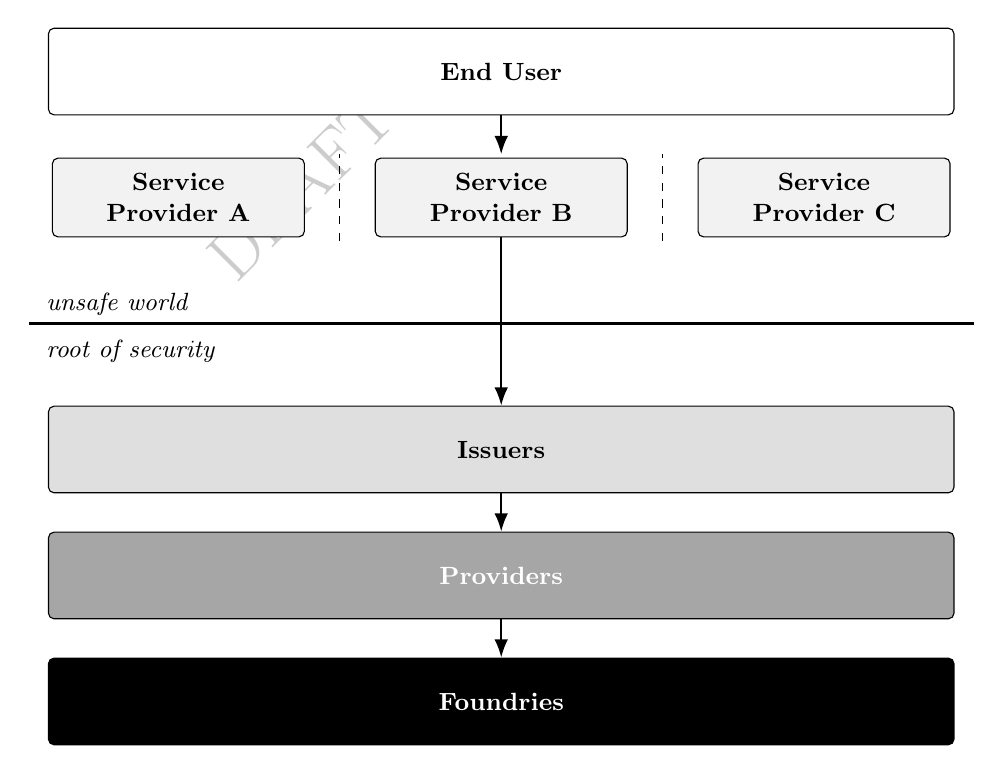
\begin{tikzpicture}[
    stack/.style={
      draw,
      rounded corners=2pt,
      minimum width=11.5cm,
      minimum height=1.1cm,
      align=center,
      font=\small
    },
    sp/.style={
      draw,
      rounded corners=2pt,
      minimum width=3.2cm,
      minimum height=1cm,
      align=center,
      font=\small
    },
    label/.style={font=\small\itshape},
    >=Latex
  ]
    \node[stack, fill=white] (user) at (0,4.8) {\textbf{End User}};

    \node[sp, fill=gray!10] (sp1) at (-4.1,3.2) {\textbf{Service}\\\textbf{Provider A}};
    \node[sp, fill=gray!10] (sp2) at (0,3.2) {\textbf{Service}\\\textbf{Provider B}};
    \node[sp, fill=gray!10] (sp3) at (4.1,3.2) {\textbf{Service}\\\textbf{Provider C}};

    \draw[dashed] (-2.05,2.65) -- (-2.05,3.75);
    \draw[dashed] (2.05,2.65) -- (2.05,3.75);

    \draw[thick] (-6.0,1.6) -- (6.0,1.6);
    \node[label, anchor=west] at (-5.9,1.85) {unsafe world};
    \node[label, anchor=west] at (-5.9,1.25) {root of security};

    \node[stack, fill=gray!25] (issuer) at (0,0.0) {\textbf{Issuers}};
    \node[stack, fill=gray!70, text=white] (provider) at (0, -1.6) {\textbf{Providers}};
    \node[stack, fill=black, text=white] (foundry) at (0,-3.2) {\textbf{Foundries}};

    \draw[->, thick] (user.south) -- (0,3.75);
    \draw[->, thick] (sp2.south) -- (issuer.north);
    \draw[->, thick] (issuer.south) -- (provider.north);
    \draw[->, thick] (provider.south) -- (foundry.north);
  \end{tikzpicture}
  \caption{Trust stack around a secure element, from foundries up to end-user-facing services.}
  \label{fig:trust-stack-actors}
\end{figure}

This decomposition clarifies the reading of the rest of the chapter. The
external communication path is studied primarily because it is the current
entry point of the prototype and therefore the first concrete attack surface.
The kernel-facing and inter-service surfaces are equally important for the
target architecture, because the long-term goal is to host mutually isolated
Rustlets or applications that may originate from distinct and potentially
hostile service providers.

Not every actor category defined in Chapter~1 appears as an attacker category
here. Providers and issuers remain relevant for trust assumptions and
administrative authority, but the present chapter focuses on the interfaces
through which end users, service providers and hardware-origin adversaries can
actually attack the platform.

Figure~\ref{fig:trust-stack-actors} summarizes the actors involved in that trust
stack, but the position of an organization in the lifecycle does not by itself
make all of its software trusted. End users and service providers consume the
security properties sought by the platform. Issuers, image integrators,
provisioning authorities, toolchain operators, and hardware providers form the
pre-issuance chain of trust to the extent that they can alter or approve the
initial image and its trust anchors. The service-provider layer is intentionally
shown as multiple parallel boxes because the target architecture must support
coexistence of mutually isolated service-provider payloads within one secure
element, whereas the end-user layer is represented by a single box because one
deployed secure element is operated in one end-user context at a time.

An ordinary Rustlet remains outside the runtime TCB whether it is loaded before
or after issuance. Its developer does not become a trusted authority merely
because that Rustlet is pre-deployed. The authority that selects the Rustlet,
approves its inclusion, and produces the issued image is, however, part of the
pre-issuance chain of trust. Privileged kernel-resident modules and Security
Domain authorization logic have the more specific TCB status defined in
Chapter~1.

%--------------------------------------------------
\section{Scope and Assets}

This section defines the assets that must be protected by the platform. These
assets correspond to both data and control structures that are critical to the
security and integrity of the system.

\begin{itemize}
\item Integrity of the application lifecycle
\item Confidentiality and integrity of cryptographic keys
\item Isolation between applications
\item Integrity of the internal registry
\item Control over administrative channels
\end{itemize}

Across the three attack surfaces introduced above, these assets are exposed in
different ways: APDU-facing adversaries target command authorization and data
confidentiality, service-provider-facing adversaries target isolation and
kernel mediation, and hardware-origin adversaries would ultimately target the
root secrets on which all higher layers depend.

The integrity of the application lifecycle is the objective that operations
such as LOAD, INSTALL and DELETE must not be performed in an unauthorized or
inconsistent manner. Attacks targeting lifecycle management
have been demonstrated in smart card environments where logical flaws allow
inconsistent states or unauthorized installation flows
\cite{mostowski2008malicious, barbu2010javacard}.

The confidentiality and integrity objective for cryptographic keys requires
that sensitive material used for secure channels or internal services be
accessible and modifiable only through authorized interfaces. Numerous works
on Trusted Execution Environments and secure elements
highlight practical key extraction or misuse vulnerabilities when isolation or
API design is flawed \cite{shakevsky2022keymaster, busch2020trustedcore}.

Isolation between applications is intended to prevent one application from
interfering with or observing the execution of another. Violations of such
isolation have been widely studied in both Java Card and TEE contexts
\cite{mostowski2008malicious, cerdeira2022rezone}.

The integrity objective for the internal registry requires identifiers, states,
and privileges associated with applications and domains to remain consistent
and modifiable only through kernel-mediated transitions. Corruption or
manipulation of such metadata can lead to privilege
escalation or inconsistent system states, as observed in several TEE
vulnerability analyses \cite{munoz2023tee}.

Control over administrative channels is intended to ensure that only an entity
holding the required credentials and authority can cause management commands to
take effect. Replay, impersonation, message modification, and relay are distinct
communication threats: authentication and freshness can address the first
three, whereas a transparent real-time relay requires additional proximity or
channel-binding mechanisms that are not currently provided by oXiDe SE
\cite{roland2012relay, francis2011relay}.

General service availability is not treated as a separate asset in this model.
APDU processing is sequential, command buffers are bounded, and Rustlets use
statically constrained volatile resources, so an application cannot accumulate
unbounded APDUs or RAM allocations. Persistent storage has a narrower progress
objective: journal updates should preserve a previous valid state, and a
Rustlet whose serialized state remains within its assigned capacity should
remain rewritable. A genuine increase beyond that capacity may legitimately
return an out-of-memory error. Chapter~6 describes the persistence mechanism
against which this objective is assessed.

%--------------------------------------------------
\section{Adversary Model}

This section describes the capabilities of potential adversaries interacting
with the platform.

\begin{itemize}
\item External adversary with communication access
\item Malicious internal application
\item Compromised administrator
\end{itemize}

These adversary classes map directly onto the lifecycle-based panorama. The
external adversary corresponds to the end-user side attack surface. The
malicious internal application corresponds to the service-provider side attack
surface once independently deployed services are considered. The compromised
administrator overlaps with issuer- or provider-level operational authority and
therefore informs the privilege and trust boundaries around lifecycle
management.

The external adversary with communication access is able to send arbitrary APDU
commands to the platform and observe responses. This includes the ability to
inject malformed or malicious command sequences, attempt replay of previously
observed exchanges, or interact with the system through a man-in-the-middle
position on the communication channel. Such capabilities are illustrated by
relay and communication-layer attacks against secure elements and contactless
systems \cite{roland2012relay, francis2011relay, zhao2021sim}.

The malicious internal application corresponds to an application that has been
successfully installed but behaves in a hostile manner. Such an application may
attempt to escalate its privileges, access resources belonging to other
applications, or violate secure-storage boundaries, in particular by targeting
key management mechanisms or sensitive persistent data. These behaviors are
well documented in Java Card and TEE environments \cite{mostowski2008malicious,
barbu2010javacard, lanet2012handson, bouffard2012nightmare, bouffard2015cft,
busch2020trustedcore}.

The compromised administrator represents an entity that legitimately holds
administrative privileges but uses them in a malicious or unintended way. Its
capabilities depend on which authority is compromised. A supplementary
Security Domain may misuse the powers delegated over its own administrative
subtree; the kernel is intended to prevent it from escaping that subtree or
bypassing platform-wide invariants. Compromise of the issuer, image-production
authority, or configured root authority has a substantially larger impact and
may invalidate the initial policy itself. The model therefore does not treat
``administrator'' as one uniform privilege level. Similar threat patterns are
studied in TEE privilege models and their misuse
\cite{cerdeira2022rezone, munoz2023tee}.

%--------------------------------------------------
\section{Trust Assumptions}

This section states the assumptions required for the architecture to pursue its
security objectives.

\begin{itemize}
\item Trusted root of execution
\item Correct implementation of cryptographic primitives
\item Secure key storage
\item Integrity of the runtime environment
\end{itemize}

The trusted root of execution assumes that the initial boot process and trusted
code base cannot be altered by an adversary. The runtime TCB is the one defined
in Chapter~1: the target execution substrate, kernel, privileged kernel-resident
modules, relevant Security Domain authorization logic, trust anchors, and
security configuration. This assumption is common in secure element and TEE
architectures.

Before issuance, the compiler, image-construction tools, provisioning process,
image-approval authorities, and hardware supply chain must also behave as
expected. They are dependencies of the initial trusted image rather than
resident components of its runtime TCB. Ordinary Rustlets and their developers
remain outside that TCB, including when an integration authority chooses to
pre-deploy such a Rustlet.

The correct implementation of cryptographic primitives assumes that algorithms
such as AES or MAC computations are implemented without flaws and behave as
expected. However, numerous works have shown that even correct algorithms can
leak information through side channels \cite{kocher1996timing, kocher1999dpa}.

Secure key storage assumes that cryptographic material cannot be extracted or
modified outside of authorized interfaces. Violations of this assumption have
been demonstrated in practice in TEE implementations \cite{bouffard2014reverse,
shakevsky2022keymaster}.

The integrity of the runtime environment assumes that the execution context
enforces isolation and prevents arbitrary code execution outside controlled
mechanisms.  Attacks breaking such assumptions have been demonstrated through
both fault-assisted techniques, which enable control-flow deviation or type
confusion in smart card environments \cite{dubreuil2012fault,
razafindralambo2012virus}, and logical vulnerabilities in Trusted Execution
Environments, allowing privilege escalation or interface abuse
\cite{busch2024globalconfusion}.

%--------------------------------------------------
\section{Attack Surfaces}

This section identifies the main interfaces through which an adversary may interact with the system.

\begin{itemize}
\item APDU communication interface
\item Secure channel protocol
\item Administrative command set
\item Inter-application invocation mechanisms
\item Internal registry and persistence layer
\end{itemize}

These interfaces refine the three attack surfaces of Section~2.1. The APDU
communication interface and the secure channel protocol belong to the end-user
side entry points. The administrative command set, inter-application
invocation mechanisms, and registry-facing operations become especially
relevant on the service-provider side, where a hostile deployed component may
try to cross the kernel boundary or abuse an explicit sharing interface.

On the RP2350, the current Pico~2 port starts oXiDe SE in the processor's Secure
state, but it does not yet configure a complete Secure/Non-secure TrustZone
partition or expose the final virtual-Secure-Element interface. Completing that
integration is planned for the beta~1 development cycle. In that future
configuration, the Non-secure world and its operating system must be treated as
potentially hostile, and every Secure-world entry point becomes an additional
external attack surface.

The APDU communication interface is the primary entry point and therefore the
main attack surface, as all external commands are received through this
interface. Communication-level attacks such as relay or replay attacks directly
target this interface \cite{roland2012relay}.

The secure channel protocol represents a critical surface where errors in
authentication, key derivation or message protection could compromise the
entire system. Weaknesses in secure channel implementations have historically
led to severe compromises.

The administrative command set includes operations such as INSTALL, LOAD or
DELETE, which directly impact the system state and must be strictly controlled.
Logical attacks exploiting these commands have been demonstrated in smart card
environments \cite{barbu2010javacard, lanet2012handson}.

Where explicit inter-application invocation mechanisms are provided, they allow
applications to interact and may be exploited if isolation or access control is
insufficient. They are therefore a target-architecture surface, not a claim
that every current image exposes such an interface. Such weaknesses are well
documented in both Java Card and TEE contexts
\cite{mostowski2008malicious, cerdeira2022rezone}.

The internal registry and persistence layer store critical metadata and
represent a target for tampering or corruption attacks, which can lead to
persistent privilege escalation \cite{munoz2023tee}.

%--------------------------------------------------
\section{Security Goals}

This section defines the security properties that the architecture is designed
to enforce. Their implementation and validation evidence are examined in later
chapters; no formal proof is implied here.

\begin{itemize}
\item Authenticity
\item Integrity
\item Confidentiality
\item Isolation
\item Non-bypassability
\end{itemize}

Authenticity aims to ensure that only entities holding the required credentials
can issue protected administrative or operational commands. It mitigates
impersonation, but does not by itself establish physical proximity or prevent a
transparent real-time relay \cite{roland2012relay}.

Integrity aims to make modifications of system state and application code
possible only through authorized transitions. It addresses logical
modification attempts within the stated model; physical fault injection remains
out of scope \cite{boneh1997faults}.

Confidentiality aims to protect sensitive data, in particular cryptographic
keys and secure-storage contents, against unauthorized logical access.
Side-channel attacks remain out of scope \cite{kocher1999dpa}.

Isolation aims to make applications operate independently and to contain a
malicious or defective Rustlet within its mediated resources, a key requirement
highlighted in multiple Java Card and TEE attacks
\cite{mostowski2008malicious}.

Non-bypassability is the objective that privileged effects remain mediated by
the kernel and cannot circumvent the security model, a property often violated
in real-world TEE vulnerabilities \cite{cerdeira2022rezone}.

%--------------------------------------------------
\section{Mitigations and Architectural Mapping}

This section relates the identified threats to the architectural components
previously described.

\begin{itemize}
\item Secure channel protocol
\item Privilege model
\item Security Domains
\item Registry consistency mechanisms
\item Runtime isolation
\end{itemize}

The mapping is intentionally surface-oriented: secure messaging protects the
external APDU-facing boundary, Security Domains express administrative and
cryptographic authority, the kernel privilege model mediates privileged
effects, and registry consistency plus runtime isolation limit the impact of a
hostile component once code has been deployed inside the platform.

Depending on its mode, the secure channel protocol provides peer authentication,
message integrity, confidentiality, and stateful replay protection for APDU
exchanges. These properties can prevent an unauthenticated endpoint from
modifying or impersonating a protected session, but do not prevent a transparent
real-time relay without an additional proximity or channel-binding mechanism
\cite{roland2012relay}.

The privilege model is intended to restrict administrative operations to the
authority assigned to the active administrative context, addressing privilege
escalation threats observed in malicious application scenarios
\cite{mostowski2008malicious}.

Security Domains express the delegation of administrative and cryptographic
authority over application subtrees. They do not themselves enforce memory or
execution isolation: those boundaries are provided by the kernel and, where
available, the processor protection mechanisms.

Registry consistency mechanisms are designed to validate state transitions and
preserve a recoverable valid state when committing persistent changes, thereby
mitigating attacks and failures targeting internal metadata
\cite{munoz2023tee}.

Runtime isolation is intended to prevent applications from accessing or
interfering with each other's execution or data, a critical defense against
malicious applications \cite{busch2020trustedcore}.

%--------------------------------------------------
\section{Out-of-Scope Considerations}

This section explicitly defines what is not covered by the threat model.

\begin{itemize}
\item Physical attacks
\item Side-channel attacks
\item Hardware compromise
\item Correctness of an application's own behaviour
\item Security claims for QEMU-oriented builds
\end{itemize}

The out-of-scope boundary is particularly important for the hardware-origin
attack surface introduced in Section~2.1: hardware compromise and lower-level
silicon-origin attacks are explicitly excluded from the present chapter because
they could invalidate the confidentiality and integrity properties sought by
service providers.

Physical attacks, such as fault injection or probing, are not considered in
this model, although they are well studied in the literature
\cite{boneh1997faults}.

Side-channel attacks, including timing or power analysis, are also excluded,
despite their practical impact \cite{kocher1996timing, kocher1999dpa}.

Hardware compromise falls outside the scope of this architecture-level model.

Application-level correctness is not an assumption made by this threat model:
an ordinary Rustlet may be defective or malicious. Protecting that Rustlet's
own assets from its own implementation bugs is out of scope, while containing
their effects on other applications and on kernel-owned state is a platform
security objective. The same distinction applies to a pre-deployed ordinary
Rustlet; pre-issuance placement does not turn its developer into a trusted
platform authority.

No deployment-security claim is made for QEMU-oriented builds. They are
retained as development and validation tools, not as secure deployment targets.
This is particularly important because the project
uses semihosting during bring-up and debugging, and semihosting explicitly
introduces a host-assisted escape hatch that breaks the isolation assumptions
expected from a secure element style environment \cite{qemu-security,
qemu-semihosting}. The threat model therefore applies to intended hardware
deployments, not to the convenience execution environments used during
prototype development.

%--------------------------------------------------

\chapter{Communication and Protocol}
\label{ch:communication-protocol}

This chapter describes the communication model underlying a GlobalPlatform-like
environment.  It focuses on how commands are expressed, transported and
secured, and how they enable the deployment and administration of applications.

This organization reflects the architectural role of communication in
GlobalPlatform: APDUs provide the transport abstraction, GlobalPlatform
commands define the management semantics, and secure channels enforce the
security properties of these operations.

%--------------------------------------------------
\section{APDU Model}

Application Protocol Data Units (APDUs) provide the fundamental communication
abstraction between an off-card entity and the platform. In the present
document, they are not introduced as a low-level transport artifact, but as the
basic interaction unit on top of which GlobalPlatform defines its management
protocol. An APDU carries a command or a response in a compact and structured
form, while the actual management semantics is defined at a higher level by the
command set interpreted by the platform. In other words, APDUs define the shape
of the exchange, not yet its business meaning. The GlobalPlatform Card
specification relies on this separation: commands are exchanged as APDUs, while
their interpretation depends on the instruction code, the class byte, and the
current execution context. \gpref{gp-card}{§9.4, §11}

\begin{figure}[ht]
  \centering
  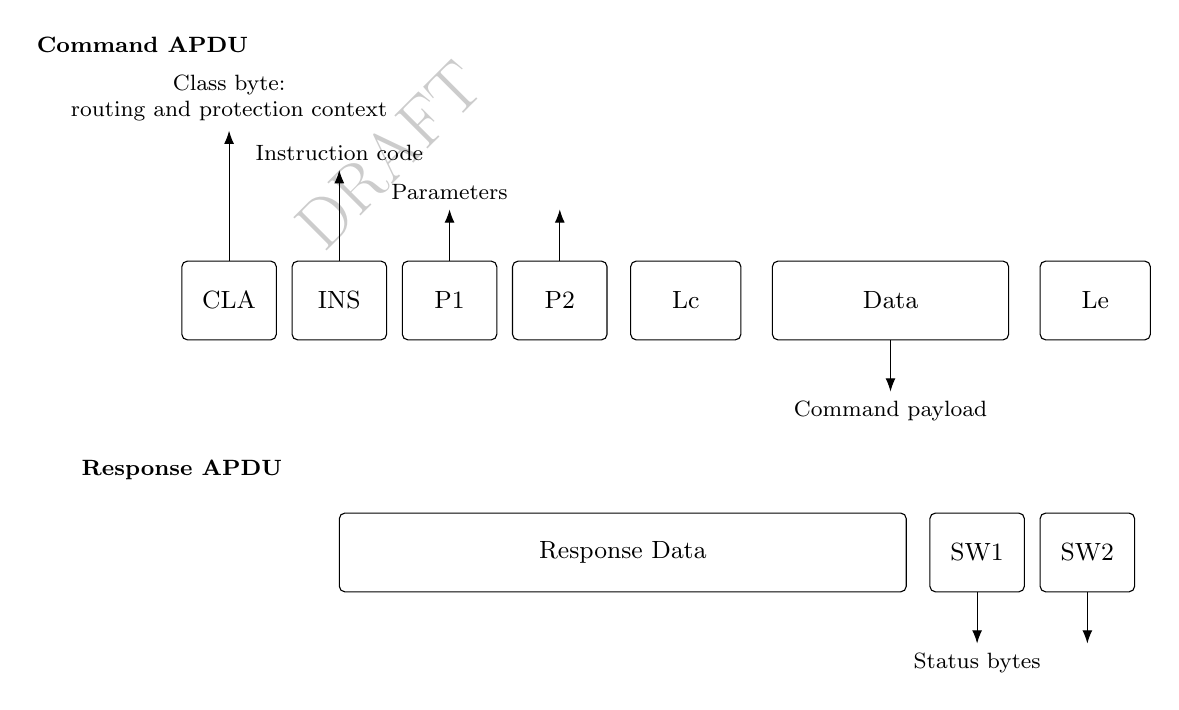
\begin{tikzpicture}[
    field/.style={
      draw,
      rounded corners=2pt,
      minimum height=1cm,
      align=center,
      font=\small
    },
    lab/.style={font=\footnotesize},
    >=Latex
  ]
    % Command APDU
    \node[lab] at (-5.9,3.25) {\textbf{Command APDU}};
    \node[field, minimum width=1.2cm] (cla) at (-4.8,0) {CLA};
    \node[field, minimum width=1.2cm] (ins) at (-3.4,0) {INS};
    \node[field, minimum width=1.2cm] (p1)  at (-2.0,0) {P1};
    \node[field, minimum width=1.2cm] (p2)  at (-0.6,0) {P2};
    \node[field, minimum width=1.4cm] (lc)  at (1.0,0) {Lc};
    \node[field, minimum width=3.0cm] (data) at (3.6,0) {Data};
    \node[field, minimum width=1.4cm] (le)  at (6.2,0) {Le};

    % Response APDU
    \node[lab] at (-5.4,-2.15) {\textbf{Response APDU}};
    \node[field, minimum width=7.2cm] (rdata) at (0.2,-3.2) {Response Data};
    \node[field, minimum width=1.2cm] (sw1) at (4.7,-3.2) {SW1};
    \node[field, minimum width=1.2cm] (sw2) at (6.1,-3.2) {SW2};

    % Annotations
    \draw[->] (cla.north) -- ++(0,1.65) node[above,align=center,font=\footnotesize] {Class byte:\\routing and protection context};
    \draw[->] (ins.north) -- ++(0,1.15) node[above,align=center,font=\footnotesize] {Instruction code};
    \draw[->] (p1.north) -- ++(0,0.65) node[above,align=left,font=\footnotesize] {Parameters};
    \draw[->] (p2.north) -- ++(0,0.65);
    \draw[->] (data.south) -- ++(0,-0.65) node[below,align=center,font=\footnotesize] {Command payload};
    \draw[->] (sw1.south) -- ++(0,-0.65) node[below,align=left,font=\footnotesize] {Status bytes};
    \draw[->] (sw2.south) -- ++(0,-0.65);

  \end{tikzpicture}
  \caption{Abstract structure of a command/response APDU pair.}
  \label{fig:apdu-abstract}
\end{figure}

Figure~\ref{fig:apdu-abstract} presents the abstract command/response structure
used throughout this document. A command APDU starts with a four-byte header
formed by the class byte (\texttt{CLA}), the instruction byte (\texttt{INS}),
and two parameter bytes (\texttt{P1}, \texttt{P2}). It may then contain a
length field (\texttt{Lc}), a data field, and an expected response length
(\texttt{Le}). The response APDU mirrors this model in a simpler form: it
returns an optional response data field followed by two status bytes
\texttt{SW1} and \texttt{SW2}, which indicate success or failure and sometimes
encode additional protocol information. This abstract view is sufficient to
understand the role of APDUs in GlobalPlatform: they provide a generic and
extensible envelope for all management operations.  \gpref{gp-card}{§9.4}
\gpref{iso7816-4}{§5, §6}

\subsection{APDU Vocabulary}

The APDU-related vocabulary used throughout this document is the
following:

\begin{itemize}
\item \textbf{command APDU}: an APDU sent by the interface device
  towards the secure element;
\item \textbf{response APDU}: an APDU returned by the secure element;
\item \textbf{header}: the four command bytes \texttt{CLA},
  \texttt{INS}, \texttt{P1}, and \texttt{P2};
\item \textbf{incoming data} or \textbf{command payload}: the bytes
  carried from the interface device to the secure element, logically measured by
  \texttt{Lc};
\item \textbf{outgoing data} or \textbf{response payload}: the bytes
  returned by the secure element before the final status, logically measured by
  \texttt{Le};
\item \textbf{status word}: the two-byte trailer \texttt{SW1/SW2};
\item \textbf{logical APDU case}: one of the four abstract APDU shapes
  (Case~1 to Case~4), independent of the concrete transport protocol;
\item \textbf{\texttt{T=0} transport}: the half-duplex,
  character-oriented transport defined by ISO/IEC~7816-3;
\item \textbf{deferred response}: the \texttt{T=0} realization of a
  logical Case~4 exchange, where response data is announced by
  \texttt{61xx} and later recovered through \texttt{GET RESPONSE};
\item \textbf{ATR}: the \emph{Answer To Reset}, i.e. the first byte
  string emitted by the secure element after activation/reset and before the APDU
  command stream starts.
\end{itemize}

\subsection{APDU Cases under T=0}

Before considering GlobalPlatform command semantics, it is useful to
distinguish the four abstract command cases that arise from the presence
or absence of incoming and outgoing data. In the short-APDU model used
throughout this document, these cases are:

\begin{itemize}
\item \textbf{Case 1 (empty)}: the command carries only the four-byte
  header and no data is exchanged beyond the final status word;
\item \textbf{Case 2 (out)}: the command carries an expected response
  length \texttt{Le}, and the secure element returns response data followed by
  \texttt{SW1/SW2};
\item \textbf{Case 3 (in)}: the command carries a command length
  \texttt{Lc} and an incoming data field, but no response data beyond
  the final status word;
\item \textbf{Case 4 (in+out)}: the command carries incoming data and
  also logically expects response data.
\end{itemize}

At the abstract APDU level, these four cases are sufficient to describe
the shape of the exchange. Their concrete serialization depends on the
transport protocol. In particular, the classical \texttt{T=0} transport
is half-duplex and does not simply carry incoming and outgoing payloads
as a single full-duplex frame. As a result, a logical ``in+out'' APDU is
usually realized in two steps: the command first transfers its incoming
payload, and if response bytes are then available, the secure element indicates
this through a status word of the form \texttt{61xx}. The interface
device must
then issue a dedicated \texttt{GET RESPONSE} command to fetch the
pending outgoing bytes.

This is the key distinction between the abstract APDU model and its
\texttt{T=0} realization. Abstractly, Case~4 remains a single command
that both consumes and produces data. Concretely, the response payload
may be deferred and retrieved by one or more \texttt{GET RESPONSE}
commands. In the classical short-\texttt{T=0} convention, pending
response bytes are announced through a status word of the form
\texttt{61xx}, and the interface device then issues \texttt{GET RESPONSE}
(\texttt{INS = C0}, conventionally with \texttt{P1 = 00} and
\texttt{P2 = 00}) to retrieve the remaining bytes.

A command that only receives data typically terminates with a final
status word, while a command that only sends data can return its payload
immediately before that final status. A logical Case~4 command is
therefore the only case that needs this extra \texttt{GET RESPONSE}
step in a \texttt{T=0} exchange. This distinction also explains why the
fifth command byte cannot be interpreted in isolation: depending on the
case, it denotes either \texttt{Lc} or \texttt{Le}.

\subsubsection{Procedure bytes and immediate status}
\label{sec:apdu-t0-procedure-bytes}

After the interface device has transmitted the five-byte command
header, it does not interpret subsequent bytes as response data
immediately. It first waits for a \texttt{T=0} procedure byte. The
following values determine the next phase of the exchange:

\begin{itemize}
\item \texttt{INS} acknowledges transfer of all remaining command or
  response data bytes;
\item the one's complement of \texttt{INS} acknowledges transfer of
  exactly one data byte;
\item \texttt{60} is the NULL procedure byte: no data is transferred
  and the interface device continues waiting;
\item a valid \texttt{SW1} value terminates the command immediately,
  and the next byte is interpreted as \texttt{SW2}.
\end{itemize}

Consequently, a secure element may reject a command directly after its
header, for example with \texttt{69 85}, without first returning the
number of bytes announced by \texttt{Le}. There is no ambiguity with
response data: response bytes are interpreted as data only after an
\texttt{INS} or complemented-\texttt{INS} ACK has opened the data
transfer phase. Once that phase is open, the interface device counts the
announced bytes before interpreting the final \texttt{SW1/SW2}.

This byte-level multiplexing constrains instruction coding. For a
command transported over \texttt{T=0}, \texttt{INS} shall not be in
\texttt{60--6F} or \texttt{90--9F}, because these ranges are reserved
for NULL, status, and related procedure-byte meanings. Oxide SE command
definitions and Rustlet applications intended for the \texttt{T=0}
interface must respect this restriction. Appendix~\ref{app:apdu-over-t0}
describes how the reference implementation realizes these
procedure-byte transitions.

A concrete serialization depends on the underlying transport case. In the
classical \texttt{T=0} model, command and response exchanges are constrained by
a byte-oriented half-duplex protocol, and the APDU structure is materialized
through a small number of normalized cases depending on the presence or absence
of data and expected response bytes.  For the purpose of this chapter, the
important point is not the detailed enumeration of those cases, but the fact
that the abstract APDU model remains stable across transport variants: the same
logical command still consists of a header, optional command data, and a
structured response.

The detailed implementation strategy of APDU transport, including the mapping
of the abstract model to the \texttt{T=0} protocol, is discussed in
Chapter~8 (Reference Implementation), Section~\ref{sec:impl-apdu-t0}
according to \gpref{gp-card}{§5.3, §9.4}. The same transport principles
remain relevant even when higher-level services such as secure messaging
later wrap the command payload.

\subsection{Reference Smart-Card Link and Serial-Line Adaptation}
\label{sec:apdu-serial-adaptation}

In the ISO/IEC~7816 reference architecture, APDUs transported with
\texttt{T=0} cross the dedicated electrical interface of a contact smart card.
The contact assignment and physical interface are specified by
ISO/IEC~7816-2, while activation, ATR exchange, character framing, timing, and
the \texttt{T=0} transmission protocol are specified by ISO/IEC~7816-3
\cite{iso7816-2,iso7816-3}. This smart-card link is therefore more than an
ordinary serial port, even though \texttt{T=0} itself is a byte-oriented,
half-duplex protocol.

Most general-purpose microcontrollers available as off-the-shelf development
boards do not expose that complete smart-card electrical form factor. To make
oXiDe SE directly usable on such hardware, the reference implementation carries
the \texttt{T=0} byte exchange over a conventional serial line. This is a
deliberate transport adaptation: it preserves the APDU command/response model,
procedure bytes, ATR, and deferred-response behavior needed by the software,
but it does not claim that a UART connection is the ISO/IEC~7816 physical
interface.

Support for the actual ISO/IEC~7816 contact interface remains a reference
porting target. The kernel architecture must consequently keep APDU and
\texttt{T=0} processing independent of the serial-line driver, so that a board
providing the required smart-card peripheral and electrical interface can
replace the UART transport without changing GlobalPlatform command handling,
secure-channel processing, or Rustlet dispatch.

\subsection{Timing Constraints of the \texttt{T=0} Exchange}
\label{sec:apdu-t0-timing}

ISO/IEC~7816 should be read here as a layered set of constraints rather
than as a single monolithic APDU document:

\begin{itemize}
\item ISO/IEC~7816-1 defines the physical card characteristics
  \cite{iso7816-1};
\item ISO/IEC~7816-2 defines the contacts and their placement
  \cite{iso7816-2};
\item ISO/IEC~7816-3 defines activation/reset, the ATR, the elementary
  time unit, character framing, guard times, waiting times, and the
  \texttt{T=0} half-duplex character transport \cite{iso7816-3};
\item ISO/IEC~7816-4 defines the APDU model, command-response
  structure, logical channels, and commands such as
  \texttt{GET RESPONSE} \cite{iso7816-4}.
\end{itemize}

For the timing points that matter to an implementation,
ISO/IEC~7816-3 is the critical standard. ISO/IEC~7816-4 then explains
the logical APDU consequences of those transport constraints.

The first timing constraint appears during activation. Public summaries
of ISO/IEC~7816-3 restate that, after clock startup and reset
assertion, the secure element must emit its ATR within a bounded clock-cycle
window: the ATR begins between 400 and 40\,000 clock cycles after the
reset event \cite{adi-smartcard-fundamentals}. This is why the standard
budget is better understood in cycles than in milliseconds. At
2~MHz, 40\,000 cycles correspond to 20~ms; at higher clock rates, the
same normatively-defined window becomes shorter in wall-clock time.

The next important point is what happens \emph{after} the ATR. The
standardized transport does not grant a millisecond-scale software pause
between the end of the ATR and the start of the next command. On the
contrary, once the ATR is complete, the secure element waits for interface-device
characters under the active transmission parameters
\cite{iso7816-3}. The timing unit is the elementary time unit
(\emph{etu}), which ISO/IEC~7816-3 defines from the transmission
parameters and the secure-element clock. Public hardware documentation also
emphasizes the same operational view: the ETU is the bit clock, a
character frame is ten bits long, and guard/wait times are also
expressed in ETUs rather than in milliseconds
\cite{microchip-iso7816-usart,microchip-guardtime}.

This has a direct implementation consequence. At default settings, the
transport leaves only the normal character pause and guard-time budget
between adjacent protocol events. In practical terms, the hot
boundaries are:

\begin{itemize}
\item the end of ATR transmission and the beginning of the first command
  reception;
\item the end of command-header reception and the beginning of incoming
  payload reception for a logical Case~3 or Case~4 exchange;
\item the end of a status-word transmission and the beginning of the
  next command reception;
\item in a deferred Case~4 exchange, the end of a \texttt{61xx}
  transmission and the beginning of the next \texttt{GET RESPONSE}
  command.
\end{itemize}

The standard also constrains the opposite side of the timing problem:
characters emitted by the secure element are subject to waiting-time limits, so long
processing excursions before a required transmission are also
protocol-sensitive \cite{iso7816-3}. The important architectural point
is therefore not merely that \texttt{T=0} is synchronous in a
``schoolbook'' sense, but that its safety margins are intentionally
small and expressed at the byte/character level.

In the current prototype, the UARTs are not physically clocked by the
ISO card clock, so the exact hardware coupling differs from a literal
contact-card implementation. Nevertheless, the software consequence is
the same: these boundaries must be treated as hot-path transitions, and
implementers should avoid inserting logging, allocation, registry work,
or any other unrelated code between transmission completion and the next
receive step. Chapter~8 returns to this point and explains how the
current implementation keeps these transitions intentionally tight
(\S\ref{sec:impl-apdu-t0}).

Among the APDU header fields, the instruction byte \texttt{INS} carries the
first level of semantic meaning. It identifies the command family to be
executed, such as \texttt{INSTALL}, \texttt{LOAD}, \texttt{DELETE}, or
\texttt{GET STATUS} in the GlobalPlatform management model. In that sense,
\texttt{INS} is best understood as an opcode: it says \emph{what kind of
operation is requested}. However, \texttt{INS} alone is not enough to determine
the full meaning of a command. The detailed interpretation also depends on the
class byte, on the parameter bytes, and on the security context in which the
command is received. This is why APDUs should not be viewed as self-describing
business messages: they are compact protocol objects whose meaning emerges from
the combination of several header fields and from the current platform state.
\gpref{gp-card}{§11}

The class byte \texttt{CLA} is more subtle and, in practice, more informative
than a simple ``protocol class'' tag. In a GlobalPlatform setting, it plays at
least three distinct roles.  First, it distinguishes command spaces, in
particular whether the command is interpreted as an ISO-style command or as a
GlobalPlatform management command. The specification explicitly uses
ranges of \texttt{CLA} values to discriminate these cases. Second, the class
byte carries the logical channel number, in accordance with ISO/IEC~7816-4.
GlobalPlatform states that logical channel information shall be indicated in
the class byte of the command header, so the same instruction may be sent on
different channels, each channel being associated with a different selected
application or execution context. Third, the class byte is also used to
indicate whether secure messaging is applied to the command. In particular,
GlobalPlatform secure channel mechanisms modify the class byte to signal that
the APDU is protected, while the exact bit pattern depends on the logical
channel encoding and on the secure messaging mode.  \gpref{gp-card}{§9.4,
§11.3} \gpref{scp03}{§7}

The logical channel mechanism is important because it separates communication
contexts without changing the command vocabulary itself. A command is still
identified by its instruction code, but the \texttt{CLA} byte specifies on
which logical channel it is sent. From an architectural point of view, this
means that the APDU model already contains a lightweight routing mechanism: the
off-card entity does not only request an operation, it also addresses the
execution context in which this operation must be interpreted. This is
particularly relevant when several applications or management contexts coexist
on the same secure element. The GlobalPlatform Card Specification therefore treats the
logical channel information carried by \texttt{CLA} as part of the command
dispatching context. \gpref{gp-card}{§9.4}

The same byte also supports secure messaging. When a Secure Channel is active,
a command APDU is no longer a plain protocol object: it becomes a protected
message whose header and payload must be interpreted together with the
cryptographic context of the session. In SCP03, for example, the command header
is modified so that the class byte indicates that secure messaging is present;
the command may then include a command MAC and, depending on the requested
security level, encrypted command data. The specification also explains how
this marking interacts with logical channel information. Thus, the \texttt{CLA}
byte should be understood as the place where routing information and protection
state meet: it tells the platform both \emph{where} the command is addressed
and \emph{whether} it is protected. \gpref{gp-card}{§9.4} \gpref{scp03}{§7.1}

The APDU model is deliberately generic: its structure is stable and compact,
but most of the management meaning is not encoded in the shape of the message
itself. Instead, that meaning is reconstructed from three layers of
interpretation: the abstract APDU format, the command semantics associated with
the GlobalPlatform instruction set, and the security context associated with
secure messaging.  This separation is precisely what makes APDUs a suitable
foundation for a GlobalPlatform-like environment: they are generic enough to
transport very different commands, yet structured enough to support routing,
session protection, and administration semantics within a single uniform model.

From an implementation perspective, this layered interpretation of APDUs
directly translates into distinct software components. The concrete design
choices for parsing, dispatching and secure channel integration are discussed
in Chapter~8 (Reference Implementation).

%--------------------------------------------------
\section{GlobalPlatform Command Model}

GlobalPlatform defines a set of card management commands that give semantic
meaning to APDU exchanges. These commands are used to deploy, configure, manage
and query applications hosted on the platform. They are specified in the
GlobalPlatform Card Specification, which defines both their semantics and their
encoding within the APDU structure \gpref{gp-card}{§11, §11.9}.

Unlike the APDU model, which only defines a generic communication structure,
the GlobalPlatform command model defines a protocol of orchestration. Each
command corresponds to a well-defined operation on the internal state of the
secure element, such as loading executable content, installing an application,
managing keys or querying the registry. The specification explicitly organizes
these commands as \emph{card management commands}, executed under the authority
of a Security Domain \gpref{gp-card}{§7, §11}.

An important property of this model is that commands operate on opaque
payloads. GlobalPlatform does not define the binary format of applications;
instead, it defines how such binaries are transported, installed and managed
through sequences of APDUs. In particular, the loading process is defined as a
sequence of \texttt{LOAD} commands followed by \texttt{INSTALL} operations,
independently of the internal structure of the code being deployed
\gpref{gp-card}{§11.6, §11.7}.

Commands are not always used in isolation but are often composed into
higher-level workflows aligned with the application lifecycle. For instance,
application deployment typically involves secure channel establishment,
load-file loading, application installation and activation. These flows are implicitly
defined by the specification through command preconditions and state
transitions \gpref{gp-card}{§9, §11}.

From an architectural perspective, the command model also defines a separation
between identification, authorization and execution. Commands are addressed to
a given context (through the APDU model), executed under a Security Domain, and
validated against privilege and lifecycle constraints defined by the platform
\gpref{gp-card}{§7, §9.6}.

The detailed implementation of command parsing, dispatch, validation and
execution policies is out of scope of this chapter and is described in
Chapter~8 (Reference Implementation), Section~\ref{sec:impl-apdu-dispatch}.

\subsection{Command Overview}

The GlobalPlatform management model defines a set of APDU-based commands
used to control the lifecycle of applications, manage cryptographic material,
and interact with the internal state of the secure element. These commands are
specified in the GlobalPlatform Card Specification and are collectively
referred to as \emph{card management commands} \gpref{gp-card}{§11}.

From an architectural perspective, these commands can be grouped into several
categories according to their role in the system.

\paragraph{Application and Load File Lifecycle Management}

These commands are used to deploy, install, activate and remove application
code:

\begin{itemize}
\item \textbf{LOAD}: Transfers executable content (typically in multiple
    fragments) to the secure element.
\item \textbf{INSTALL}: Creates and configures application instances, and
    optionally makes them selectable.
\item \textbf{DELETE}: Removes application instances or load files from the secure
    element.
\item \textbf{SET STATUS}: Updates the lifecycle state of applications or
    Security Domains.
\item \textbf{GET STATUS}: Retrieves information about installed entities and
    their states.
\end{itemize}

These commands define the operational workflow of application deployment and
lifecycle management \gpref{gp-card}{§11.6, §11.7, §11.9} described in
Chapter~8, Section~\ref{sec:impl-lifecycle}.

\paragraph{Security and Key Management}

These commands manage cryptographic material and secure communication:

\begin{itemize}
\item \textbf{PUT KEY}: Installs or updates cryptographic keys within a
    Security Domain.
\item \textbf{INITIALIZE UPDATE}: Initiates a secure channel session.
\item \textbf{EXTERNAL AUTHENTICATE}: Completes the establishment of a secure
    channel.
\end{itemize}

They are central to enforcing authenticity and confidentiality of management
operations \gpref{gp-card}{§9.6, §11.8} \gpref{scp03}{§6} detailed in
Chapter~8, Section~\ref{sec:impl-scp}.

\paragraph{Data Management and Configuration}

These commands provide controlled access to internal data structures:

\begin{itemize}
\item \textbf{GET DATA}: Retrieves data objects from the secure element.
\item \textbf{STORE DATA}: Sends application-specific or platform-specific
    configuration data.
\end{itemize}

They enable controlled interaction with the internal registry and application
parameters \gpref{gp-card}{§11.4, §11.5} handled as described in Chapter~8,
Section~\ref{sec:impl-registry}.

\paragraph{Context and Communication Management}

These commands control the execution context and communication channels:

\begin{itemize}
\item \textbf{SELECT}: Selects an application or Security Domain as the current
    context.
\item \textbf{MANAGE CHANNEL}: Opens or closes logical communication channels.
\end{itemize}

They define how commands are routed and interpreted within the platform
\gpref{gp-card}{§9.4} see Chapter~8, Section~\ref{sec:impl-channel}.

\medskip

Although each command has a well-defined individual semantics, they are rarely
used in isolation. Instead, they are composed into structured sequences that
implement higher-level operations. For instance, application deployment
typically involves secure channel establishment, followed by a sequence of
\texttt{LOAD} commands, and completed by an \texttt{INSTALL} command.

From a design perspective, these commands form a minimal but expressive
instruction set that allows external entities to drive the evolution of the
platform state without requiring any knowledge of the internal representation
of applications. The command model therefore acts as a stable control interface
between the external management environment and the internal execution
platform.

The concrete implementation of command grouping, sequencing constraints and
state validation mechanisms is described in Chapter~8 (Reference
Implementation), Section~\ref{sec:impl-apdu-dispatch}.

\subsection{LOAD Command}

The \texttt{LOAD} command is used to transfer executable content to the
secure element. It is part of the application deployment process and is typically
followed by an \texttt{INSTALL} command. The semantics of this command are
defined in the GlobalPlatform Card Specification \gpref{gp-card}{§11.6}.

\apdudesc
{80}
{E8}
{last-block flag}
{\#block}
{var}
{00}
{Load File Data Block fragment}
{none}

Unlike most other commands, \texttt{LOAD} is designed to handle large payloads
that cannot fit within a single APDU. As a result, the loading process is
performed through a sequence of \texttt{LOAD} commands, each carrying a
fragment of the executable content.

The \texttt{P1} parameter indicates whether the current block is the last one
(bit~8), while \texttt{P2} carries the block number. This allows the secure
element to reconstruct the full load file incrementally.

The concatenated payload contains a Load File Data Block, normally a
\texttt{C4} BER-TLV object whose value is the executable load file. The
executable value remains opaque to GlobalPlatform: the specification defines
its transport envelope and sequence, not the implementation-specific binary
format carried inside it.

The \texttt{LOAD} command is therefore not an atomic operation but part of a
higher-level transactional process. The platform must ensure that partial or
inconsistent loading sequences do not result in a corrupted state. In
particular, the complete sequence must be validated before the loaded content
becomes usable.

On success, the secure element returns status word \texttt{90 00}. Other status values
may indicate:
\begin{itemize}
\item \texttt{6A80}: invalid data (malformed fragment)
\item \texttt{6985}: conditions not satisfied (e.g., missing secure channel)
\item \texttt{6A84}: insufficient memory
\item \texttt{6581}: memory failure
\end{itemize}

The handling of fragmentation, buffering, integrity checks, and
transactional guarantees remains implementation-dependent. It is
described in Chapter~8 (Reference Implementation),
Section~\ref{sec:impl-load}.

\subsection{INSTALL Command}
\label{sec:gp-install-command}

The \texttt{INSTALL} command is used to create, configure and optionally
activate an application instance on the secure element. It is the central
operation that completes the application deployment process after the transfer
of executable content through \texttt{LOAD} commands. Its semantics are defined
in the GlobalPlatform Card Specification \gpref{gp-card}{§11.7}.

\apdudesc
{80}
{E6}
{mode}
{flags}
{var}
{00}
{AIDs and installation parameters}
{none}

Unlike \texttt{LOAD}, which is concerned with data transfer, \texttt{INSTALL}
operates at the level of the platform state. It binds previously loaded
executable content to an application instance, associates identifiers, defines
privileges and establishes the execution context.

The \texttt{P1} parameter specifies the installation mode. Depending on its
value, the command may perform different operations such as installation for
load, installation for install, installation for make selectable, or a
combination of these. This makes \texttt{INSTALL} a polymorphic command whose
behavior depends on control flags rather than a single fixed semantics.

The payload contains several identifiers, including:
\begin{itemize}
\item the Executable Load File AID
\item the application (or instance) AID
\item the Security Domain AID under which the application is installed
\item optional installation parameters
\end{itemize}

These elements define how the application is registered and under which
authority it operates. The interpretation of installation parameters is left to
the execution environment and is not specified by GlobalPlatform.

The \texttt{INSTALL} command also plays a critical role in privilege
assignment. It is through this command that an application may be granted
specific capabilities, such as delegated management rights or access to secure
services. These privileges are enforced by the Security Domain model
\gpref{gp-card}{§7, §11.7}.

On success, the secure element returns status word \texttt{90 00}. Other status values
may indicate:
\begin{itemize}
\item \texttt{6A80}: invalid data (incorrect AID or parameters)
\item \texttt{6985}: conditions not satisfied (e.g., missing prerequisites)
\item \texttt{6982}: security status not satisfied
\item \texttt{6A84}: insufficient memory
\end{itemize}

From a protocol perspective, \texttt{INSTALL} terminates the loading sequence
and makes the application available to the platform, either immediately or
after an explicit lifecycle transition.

The detailed implementation of installation semantics, including registry
updates, privilege assignment and lifecycle transitions, is described in
Chapter~8 (Reference Implementation), Section~\ref{sec:impl-install}.

\subsection{DELETE Command}

The \texttt{DELETE} command is used to remove application instances or load
files from the secure element. It is part of the application lifecycle management and
complements the \texttt{LOAD} and \texttt{INSTALL} commands by enabling the
removal of previously deployed content. Its semantics are defined in the
GlobalPlatform Card Specification \gpref{gp-card}{§11.9}.

\apdudesc
{80}
{E4}
{00}
{flags}
{var}
{00}
{AID(s) to delete}
{none}

The command operates on one or more identifiers provided in the payload,
typically Application Identifiers (AIDs) corresponding to application instances,
load files, or Security Domains. \texttt{P1} is zero. Depending on the control
flags encoded in \texttt{P2}, the command may delete:
\begin{itemize}
\item a specific application instance
\item a complete load file (including all associated instances)
\item a Security Domain and its subordinate hierarchy through cumulative deletion
\end{itemize}

Unlike \texttt{INSTALL}, which introduces new state, \texttt{DELETE} removes
entries from the internal registry and releases associated resources such as
memory and identifiers.

The operation is subject to strict constraints. In particular:
\begin{itemize}
\item an application cannot be deleted while it is selected on another
      logical channel
\item a load file cannot be removed if dependent applications still exist
\item appropriate privileges must be held by the invoking Security Domain
\end{itemize}

These constraints ensure the consistency of the platform state and prevent
partial or inconsistent removal operations.

On success, the secure element returns status word \texttt{90 00}. Other status values
may indicate:
\begin{itemize}
\item \texttt{6A88}: referenced data not found
\item \texttt{6985}: conditions not satisfied
\item \texttt{6982}: security status not satisfied
\item \texttt{6A84}: not enough memory or resources to complete the operation
\end{itemize}

From an architectural perspective, \texttt{DELETE} is a destructive operation
that must preserve system integrity. It requires validation of dependencies and
enforcement of lifecycle constraints before state modification.

The detailed implementation of dependency checking, registry updates and
resource cleanup is described in Chapter~8 (Reference Implementation),
Section~\ref{sec:impl-delete}.

\subsection{SET STATUS Command}

The \texttt{SET STATUS} command is used to update the lifecycle state of an
object managed by the platform, such as an application, a load file or a
Security Domain. It plays a key role in controlling the activation and
deactivation of components. Its semantics are defined in the GlobalPlatform
Card Specification \gpref{gp-card}{§11.9}.

\apdudesc
{80}
{F0}
{type}
{state}
{var}
{00}
{AID of target object}
{none}

The command operates on a target object identified by its AID, provided in the
payload.  The \texttt{P1} parameter specifies the type of object being
addressed, while the \texttt{P2} parameter encodes the state-control operation.
The Oxide SE reference profile accepts:

\begin{center}
\begin{tabular}{p{0.20\textwidth}p{0.52\textwidth}}
\textbf{Field value} & \textbf{Meaning} \\
\hline
\texttt{P1 = 20} & package / executable load-file object; \\
\texttt{P1 = 40} & ordinary application instance; \\
\texttt{P1 = 80} & Security Domain instance; \\
\texttt{P2 = 80} & lock the addressed object; \\
\texttt{P2 = 00} & unlock the addressed object into its usable state.
\end{tabular}
\end{center}

Typical lifecycle states depend on the object family and on the selected
platform profile. The Oxide SE lifecycle subset used by the reference model is
defined in Section~\ref{sec:gp-lifecycle-model}: packages are
\emph{Loaded} or \emph{Locked}, application instances and Security Domains are
\emph{Selectable} or \emph{Locked}, and key objects are \emph{Active} or
\emph{Locked}. \texttt{SET STATUS} controls packages, application instances,
and Security Domains. Key-object lifecycle is controlled by key-management
commands, not by \texttt{SET STATUS}.

The different object types manipulated by the platform, as well as their
associated attributes, are defined in Section~\ref{sec:gp-object-model}. Their
lifecycle states and valid transitions are described in
Section~\ref{sec:gp-lifecycle-model}.

Lifecycle transitions are not arbitrary. The platform enforces a state machine
that restricts valid transitions and ensures consistency. For example, a locked
package cannot be instantiated, a locked application cannot be selected, and a
locked Security Domain cannot be used to establish a secure channel.

The execution of \texttt{SET STATUS} is subject to strict access control. Only
authorized Security Domains holding the appropriate privileges may modify
lifecycle states \gpref{gp-card}{§7, §11.9}.
Oxide SE additionally applies the following reference policy: the target
object must be under the authority of the Security Domain used for the command;
protected commands use the Security Domain bound to the active secure channel;
clear commands use the root Security Domain and are accepted only when that
Security Domain explicitly allows \texttt{SET STATUS} without SCP. The
development \texttt{NullSecurityDomain} allows this bypass; production
Security Domains do not.

On success, the secure element returns status word \texttt{90 00}. Other status values
may indicate:
\begin{itemize}
\item \texttt{6A80}: invalid parameters (unsupported state transition)
\item \texttt{6985}: conditions not satisfied
\item \texttt{6982}: security status not satisfied
\end{itemize}

From an architectural perspective, \texttt{SET STATUS} is a control command
that governs the visibility and usability of objects without modifying their
underlying content.

The detailed implementation of lifecycle state machines and transition
validation is described in Chapter~8 (Reference Implementation),
Section~\ref{sec:impl-lifecycle}.

\subsection{GET DATA Discovery Objects}
\label{sec:gp-get-data-discovery}

Before opening a secure channel, a host must be able to discover the
administrative protocols offered by the selected Security Domain. The
GlobalPlatform discovery path uses \texttt{GET DATA}; it does not require the
host to probe establishment commands until one happens to succeed
\gpref{gp-card}{§11.3, §11.4}.

\apdudesc
{80}
{CA}
{tag high}
{tag low}
{00}
{var}
{none}
{requested data object}

\paragraph{Card Recognition Data: tag \texttt{0066}.}

The response is a BER-TLV object \texttt{66} containing a Card Recognition
Data template \texttt{73}. Its minimum useful GlobalPlatform structure is:

\begin{verbatim}
66 LL
   73 LL
      06 07 2A 86 48 86 FC 6B 01
      60 0B 06 09 2A 86 48 86 FC 6B 02 02 03
      63 09 06 07 2A 86 48 86 FC 6B 03
      64 0B 06 09 2A 86 48 86 FC 6B 04 scp i
      ...
\end{verbatim}

The first three OIDs identify the GlobalPlatform recognition authority, the
Card Specification version, and the card-identification scheme. Each
\texttt{64} template then advertises one Secure Channel Protocol through the
OID \texttt{\{globalPlatform 4 scp i\}}. Several \texttt{64} templates may be
present. For the Oxide SE profile:

\begin{itemize}
\item SCP03 is identified by \texttt{scp = 03}; \texttt{i = 00} advertises
      S8 and \texttt{i = 01} advertises S16, using random challenges and
      without a separately initiated R-MAC session;
\item SCP11 is identified by \texttt{scp = 11}; \texttt{i} is a bitmap whose
      bits select SCP11a, SCP11b and SCP11c, with bit~7 set for the S16
      profile. Therefore SCP11a+c is advertised as \texttt{i = 51}, and
      SCP11a+b+c as \texttt{i = 53}.
\end{itemize}

An Issuer Security Domain intended for production shall advertise the SCPs it
actually accepts. A development-only authority that implements no secure
channel may return the same well-formed recognition structure without a
\texttt{64} template. A supplementary Security Domain may also include its
\texttt{73} recognition data in the proprietary part of its \texttt{SELECT}
response; \texttt{GET DATA 0066} remains the explicit discovery command.

\paragraph{Card Capability Information: tag \texttt{0067}.}

The optional object \texttt{67} provides more detailed capabilities. Each
supported SCP is represented by an \texttt{A0} template:

\begin{verbatim}
67 LL
   A0 LL 80 01 scp 81 LL i... [82 LL supported-key-bitmap]
   ...
   82 03 privilege-bytes
   83 01 load-file-data-block-hash
\end{verbatim}

Tag \texttt{80} identifies the SCP, tag \texttt{81} lists its supported
parameter values, and the SCP03-specific tag \texttt{82} identifies supported
static key types. The outer tag \texttt{82} reports the three-byte application
privilege model and tag \texttt{83} reports the Load File Data Block Hash
algorithm. Absence of this optional data object is reported as
\texttt{6A88}; it must not be replaced by invented capabilities.

The implementation-side construction of these objects is described in
Chapter~8, Section~\ref{sec:impl-gp-discovery}.

\subsection{GET STATUS Command}

The \texttt{GET STATUS} command is used to retrieve information about objects
managed by the platform, such as applications, load files and Security Domains.
It provides a structured view of the internal registry and is essential for
platform introspection. Its semantics are defined in the GlobalPlatform Card
Specification \gpref{gp-card}{§11.9}.

\apdudesc
{80}
{F2}
{object family}
{continuation/format}
{var}
{00}
{\texttt{4F} AID criterion, optional \texttt{5C}}
{\texttt{E3} status records}

\texttt{P1} selects the object family:

\begin{center}
\begin{tabular}{p{0.18\textwidth}p{0.60\textwidth}}
\textbf{P1} & \textbf{Objects requested} \\
\hline
\texttt{80} & Issuer Security Domain; \\
\texttt{40} & applications and supplementary Security Domains; \\
\texttt{20} & executable load files; \\
\texttt{10} & executable load files and their modules.
\end{tabular}
\end{center}

The modern TLV response format sets \texttt{P2.b2}. A first request therefore
uses \texttt{P2 = 02}; if the response ends with \texttt{63 10}, the host sends
the same query with \texttt{P2 = 03} to request the next occurrence. The
command data starts with a mandatory \texttt{4F} search criterion. Its value
may be empty, an exact AID, or an AID prefix. An optional \texttt{5C} tag list
may request particular response fields.

Each returned object is a constructed \texttt{E3} record. Its mandatory and
family-specific fields include:
\begin{itemize}
\item \texttt{4F}: object AID;
\item \texttt{9F70}: lifecycle state;
\item \texttt{C5}: three-byte privileges for an application or Security
      Domain;
\item \texttt{C4}: executable-module or package association when applicable;
\item \texttt{CC}: associated Security Domain;
\item \texttt{84}: module AID for the load-file-and-modules query.
\end{itemize}

The \texttt{GET STATUS} command is a read-only operation but is still subject
to access control. An authority sees only objects associated directly or
indirectly with its Security Domain hierarchy. In oXiDe SE the Global Registry
form is recognized only at the technical-root APDU boundary and invokes this
same lookup with the root as authority; no privilege bit bypasses subtree
filtering. Keys and private data objects are not registry status entries
exposed by this command.

On success, the secure element returns status word \texttt{90 00} along with the response
data.  Other status values may indicate:
\begin{itemize}
\item \texttt{63 10}: more matching records are available;
\item \texttt{6A88}: no matching object found
\item \texttt{6982}: security status not satisfied
\item \texttt{6A86}: incorrect \texttt{P1}/\texttt{P2}
\item \texttt{6A80}: malformed query data
\end{itemize}

From an architectural perspective, \texttt{GET STATUS} exposes a controlled
view of the internal state of the platform. It allows external entities to
observe the system without modifying it, and is therefore complementary to
lifecycle management commands.

The detailed implementation of registry traversal, filtering and response
encoding is described in Chapter~8 (Reference Implementation),
Section~\ref{sec:impl-get-status}.

\subsection{PUT KEY Command}

The \texttt{PUT KEY} command is used to install or update cryptographic keys within a
Security Domain. It is a central mechanism for managing the secure channel infrastructure
and enforcing cryptographic policies on the platform. Its semantics are defined in the
GlobalPlatform Card Specification \gpref{gp-card}{§11.8}.

\apdudesc
{80}
{D8}
{old key ver./chain}
{id./multiple}
{var}
{00}
{key data and attributes}
{none}

The command allows the caller to introduce new keys or replace existing ones. These keys
are typically used for secure channel establishment (e.g., SCP02 or SCP03), but may also
serve other platform-level cryptographic purposes.

The low seven bits of \texttt{P1} identify the key version being replaced (zero
when adding a key); bit~8 indicates whether another \texttt{PUT KEY} command
follows in the same operation. The low seven bits of \texttt{P2} identify the
first key, and bit~8 indicates that the command data contains several
consecutively numbered keys. The command data begins with the new key version,
then encodes each key's type, length, material and key-check value.

The payload contains the key material and associated attributes. Depending on the context,
the key data may be:
\begin{itemize}
\item encrypted under a key encryption key (KEK)
\item diversified based on secure-element-specific parameters
\item accompanied by metadata such as key type and length
\end{itemize}

The execution of \texttt{PUT KEY} is restricted to authorized Security Domains holding
appropriate privileges. Improper use of this command may compromise the entire security
model, as it directly affects the trust anchors of the platform.

On success, the secure element returns status word \texttt{90 00}. Other status values may indicate:
\begin{itemize}
\item \texttt{6A80}: invalid key data
\item \texttt{6985}: conditions not satisfied
\item \texttt{6982}: security status not satisfied
\item \texttt{6A88}: referenced key not found
\end{itemize}

From an architectural perspective, \texttt{PUT KEY} is not only a configuration command but
also a root-of-trust management operation. It defines the cryptographic material used to
protect all subsequent communications.

The detailed implementation of key storage, versioning, diversification and secure
handling is described in Chapter~8 (Reference Implementation),
Section~\ref{sec:impl-key-management}.

\subsection{INITIALIZE UPDATE Command}

The \texttt{INITIALIZE UPDATE} command initiates the establishment of a Secure
Channel between the host and the secure element. It is the first step of the
mutual authentication protocol defined by GlobalPlatform and is typically
followed by the \texttt{EXTERNAL AUTHENTICATE} command. Its behavior is
specified in the GlobalPlatform Card Specification and the Secure Channel
Protocol specifications \gpref{gp-card}{§9.6} \gpref{scp03}{§6}.

\apdudesc
{80}
{50}
{key ver.}
{00}
{08}
{var}
{host challenge (8 bytes)}
{card challenge and security data}

The command is sent by the host to request cryptographic material required to
derive session keys. It contains a host-generated random value, known as the
\emph{host challenge}, typically 8 bytes long.

Upon reception, the secure element responds with a structured payload that
includes:
\begin{itemize}
\item a fresh card challenge (random or pseudorandom value generated by the secure element)
\item key diversification data (if applicable)
\item a key version number identifying the key set in use
\item cryptographic data used to authenticate the card
\end{itemize}

This exchange allows both parties to derive a shared set of session keys, based
on:
\begin{itemize}
\item pre-shared static keys (installed via \texttt{PUT KEY})
\item exchanged random challenges (host and card)
\item optional diversification data
\end{itemize}

At this stage, the Secure Channel is not yet fully established. The host must
verify the authenticity of the card using the received cryptographic data, and
then complete the protocol using the \texttt{EXTERNAL AUTHENTICATE} command.

The response payload is structured but depends on the Secure Channel Protocol
in use (e.g., SCP02 or SCP03). GlobalPlatform defines the format of this data,
but its detailed interpretation is protocol-specific \gpref{scp03}{§6.2}.

On success, the secure element returns status word \texttt{90 00} along with the response
data.  Other status values may indicate:
\begin{itemize}
\item \texttt{6700}: incorrect host-challenge length
\item \texttt{6985}: conditions not satisfied
\item \texttt{6982}: security status not satisfied
\item \texttt{6A88}: key set not found
\end{itemize}

From an architectural perspective, \texttt{INITIALIZE UPDATE} is not a
management command but a protocol bootstrap operation. It establishes the
cryptographic context required to protect subsequent APDU exchanges.

The detailed implementation of challenge generation, session key derivation and
response formatting is described in Chapter~8 (Reference Implementation),
Section~\ref{sec:impl-scp-init}.

\subsection{EXTERNAL AUTHENTICATE Command}

The \texttt{EXTERNAL AUTHENTICATE} command completes the establishment of a
Secure Channel following the \texttt{INITIALIZE UPDATE} command. It allows the
host to prove knowledge of the shared secret and to activate secure messaging
for subsequent exchanges. Its behavior is defined in the GlobalPlatform Card
Specification and Secure Channel Protocol specifications \gpref{gp-card}{§9.6}
\gpref{scp03}{§6.3}.

\apdudesc
{84}
{82}
{sec. lvl}
{00}
{10/20}
{absent}
{host cryptogram followed by the transmitted C-MAC}
{none}

The command contains a cryptographic value, known as the \emph{host
cryptogram}, computed by the host using the session keys derived from the
\texttt{INITIALIZE UPDATE} exchange.  This value allows the secure element to
authenticate the host.

SCP03 Amendment~D protects \texttt{EXTERNAL AUTHENTICATE} itself with a
command MAC. The class byte therefore carries the secure-messaging indication
(\texttt{84} on logical channel zero), and the command data is the
profile-sized host cryptogram followed by the transmitted C-MAC. For the S8
profile, \texttt{Lc = 10}: eight bytes of host cryptogram and eight bytes of
transmitted C-MAC. For the S16 profile, \texttt{Lc = 20}: sixteen bytes of host
cryptogram and sixteen bytes of transmitted C-MAC. The C-MAC is computed from
an all-zero initial chaining value over the command header, whose \texttt{Lc}
already includes the transmitted C-MAC length, followed by the host cryptogram.
The full sixteen-byte C-MAC becomes the initial command and response MAC
chaining value for subsequent secure messaging; S8 only truncates the value on
the wire.

The \texttt{P1} parameter encodes the requested SCP03 security level for the
session. GlobalPlatform defines the following values:
\begin{itemize}
\item \texttt{00}: no command or response secure messaging;
\item \texttt{01}: C-MAC;
\item \texttt{03}: C-MAC and C-ENC;
\item \texttt{11}: C-MAC and R-MAC;
\item \texttt{13}: C-MAC, C-ENC, and R-MAC;
\item \texttt{33}: C-MAC, C-ENC, R-MAC, and R-ENC.
\end{itemize}

This parameter determines how subsequent APDUs will be protected, including
whether their payload is authenticated and/or encrypted.

Upon reception, the secure element verifies the host cryptogram using its own
derivation of the session keys. If the verification succeeds, the Secure
Channel is established and the selected security level is activated. From this
point on, APDUs exchanged between the host and the secure element are wrapped according
to the secure messaging rules defined by the selected protocol.

If cryptographic authentication fails, the command is rejected with
\texttt{63 00} and the session is not established.

On success, the secure element returns status word \texttt{90 00}. Other status values
may indicate:
\begin{itemize}
\item \texttt{6300}: authentication failed
\item \texttt{6700}: incorrect authentication-data length
\item \texttt{6982}: security status not satisfied
\item \texttt{6985}: conditions not satisfied
\item \texttt{6A80}: invalid cryptographic data
\item \texttt{6A86}: unsupported security level or incorrect \texttt{P1/P2}
\end{itemize}

From an architectural perspective, \texttt{EXTERNAL AUTHENTICATE} marks the
transition from an unauthenticated communication state to a secure,
authenticated and optionally encrypted session. It effectively activates the
protection mechanisms that will apply to all subsequent commands.

The detailed implementation of cryptogram verification, session activation and
secure messaging enforcement is described in Chapter~8 (Reference
Implementation), Section~\ref{sec:impl-scp-auth}.

%--------------------------------------------------
\section{Secure Channel Protocol}
\label{sec:protocol-scp}

The Secure Channel Protocol (SCP) defines how APDU exchanges are protected in
terms of authenticity, integrity and confidentiality. In a GlobalPlatform
environment, SCP is not a transport protocol but a security layer applied on
top of the APDU model. Its purpose is to ensure that management commands are
executed only if they originate from an authenticated entity and have not been
modified in transit.

Several variants of SCP exist. The profiles relevant to this architecture are
SCP03, which is based on pre-shared AES keys, and the SCP11 family
(SCP11a/SCP11b/SCP11c), which uses elliptic-curve key agreement to establish
the symmetric keys later used by the same GlobalPlatform secure-messaging
grammar.

It is important to state explicitly that SCP03 is a \emph{symmetric}
secure-channel protocol. Its mutual authentication and secure messaging
mechanisms are built from pre-shared AES keys and do not require RSA, ECC, or
any other asymmetric primitive. This point is easy to blur because the wider
GlobalPlatform ecosystem also discusses transport of asymmetric keys and
certificate-related operations, but these are not part of the cryptographic
core of SCP03 itself. In fact, GlobalPlatform's compact IoT configuration
identifies a minimal profile centered on the Issuer Security Domain, AES, and
SCP03 only \cite{gp-compact-iot}.

From a protocol perspective, all Secure Channel profiles introduce three main
mechanisms:
\begin{itemize}
\item a profile-specific establishment sequence;
\item session-key derivation;
\item common secure messaging for command and response protection.
\end{itemize}

%--------------------------------------------------
\subsection{Official Establishment Commands}

GlobalPlatform secure-channel establishment is expressed through ordinary APDU
commands. The commands below are the protocol-level entry points that a
Security Domain uses to open or evolve a secure channel.

\texttt{INITIALIZE UPDATE} starts SCP03 establishment.

\apdudesc
{80}
{50}
{key ver.}
{00}
{08/10}
{var}
{host challenge}
{key data, card challenge, card cryptogram}

\texttt{EXTERNAL AUTHENTICATE} completes SCP03 establishment, authenticates
the host, and selects the requested secure-messaging level.

\apdudesc
{84}
{82}
{sec. lvl}
{00}
{10/20}
{absent}
{host cryptogram followed by the transmitted C-MAC}
{none}

\texttt{PERFORM SECURITY OPERATION} is used by SCP11a/SCP11c to submit and
verify OCE certificate material before the actual key-agreement APDU.

\apdudesc
{80}
{2A}
{key ver.}
{key id.}
{var}
{00}
{\texttt{CERT.OCE.ECKA} or related security-operation data}
{none}

The command returns \texttt{6600} when certificate verification fails,
\texttt{6A80} when the command data is malformed, \texttt{6A86} when the
reference-control parameters are invalid or select a profiled-out option, and
\texttt{6A88} when the referenced CA key is unavailable.

\texttt{MUTUAL AUTHENTICATE} opens SCP11a and SCP11c. Its command data is a
BER-TLV Control Reference Template with tag \texttt{A6}; its successful
response returns card public-key material and a receipt.

\apdudesc
{80}
{82}
{key ver.}
{key id.}
{var}
{var}
{\texttt{A6} CRT with SCP11 key-agreement parameters}
{\texttt{5F49} card key material and \texttt{86} receipt}

Both SCP11 mutual-authentication forms return \texttt{6A80} for malformed CRT
or public-key data, \texttt{6A88} when a referenced ECKA key or required
identity object cannot be resolved, and \texttt{6985} when a mandatory prior
step such as OCE certificate authentication has not completed.

The SCP11b internal-authentication command opens SCP11b. Its command shape is
similar to SCP11 mutual authentication, but the profile semantics are
different: the card authenticates itself to the OCE, while OCE authorization
is provided outside the SCP11b exchange.

\apdudesc
{80}
{88}
{key ver.}
{key id.}
{var}
{var}
{\texttt{A6} CRT with SCP11b key-agreement parameters}
{\texttt{5F49} card key material and \texttt{86} receipt}

The same \texttt{6A80}/\texttt{6A88} distinction applies to SCP11b internal
authentication: malformed cryptographic input is different from a referenced
key or identity object that is not present.

Once the channel is open, ordinary commands are sent as protected APDUs. The
instruction byte remains the instruction of the logical command
(\texttt{SELECT}, \texttt{INSTALL}, application command, and so on), while the
class byte carries the secure-messaging indication. Under GlobalPlatform
Amendment~D secure messaging, encrypted or clear command data is followed
directly by the C-MAC; response data is followed directly by the R-MAC when
response protection is active. The real response status remains the APDU
\texttt{SW1/SW2} trailer.

\apdudesc
{84}
{INS}
{P1}
{P2}
{var}
{var}
{protected command data followed by C-MAC}
{protected response data followed by R-MAC, then SW1/SW2}

There is no single universal ``close secure channel'' APDU in the base flow.
The active session is normally ended by reset, by logical-channel management,
or by starting a new establishment sequence for the same Security Domain and
channel. SCP03 profiles that use the optional explicit R-MAC session commands
are described in Section~\ref{sec:rmac-session-management}; those commands do
not apply to SCP11.

%--------------------------------------------------
\subsection{SCP03 Session Establishment}

SCP03 is established through the two-step handshake composed of
\texttt{INITIALIZE UPDATE} followed by \texttt{EXTERNAL AUTHENTICATE}
\gpref{scp03}{§6}.

The \texttt{INITIALIZE UPDATE} command allows the secure element to provide:
\begin{itemize}
\item a card challenge
\item key diversification data (optional)
\item a key version identifier
\item a card cryptogram
\end{itemize}

The host uses this information, together with pre-shared keys, to derive
session keys and to verify the authenticity of the card.

The \texttt{EXTERNAL AUTHENTICATE} command completes the protocol by sending a
host cryptogram, authenticating that cryptogram with the initial C-MAC, and
selecting a security level. If verification succeeds, the Secure Channel is
activated and all subsequent APDU exchanges may be protected. The initial
C-MAC starts from a sixteen-byte zero chaining value. The full sixteen-byte
result becomes the first secure-messaging chain value, even when the S8 profile
transmits only its first eight bytes.

The resulting session is attached to the Security Domain and logical channel
on which the establishment APDUs were exchanged. A representative SCP03
sequence is shown below. The byte-level derivation inputs and chaining rules
are detailed in Appendix~\ref{app:scp-data-objects}.

\begin{verbatim}
1. SELECT the Security Domain
   C-APDU: 00 A4 04 00 Lsd <SD-AID> 00
   R-APDU: <FCI> 90 00

2. INITIALIZE UPDATE
   C-APDU: 80 50 key-version 00 Lc <host challenge> 00
   R-APDU: <key data> <key info> <card challenge> <card cryptogram> 90 00

3. EXTERNAL AUTHENTICATE
   C-APDU: 84 82 security-level 00 Lc <host cryptogram> <C-MAC>
   R-APDU: 90 00

4. Protected command
   C-APDU: 84 INS P1 P2 Lc <data or encrypted data> <C-MAC> Le
   R-APDU: <data or encrypted data> <R-MAC> SW1 SW2
\end{verbatim}

%--------------------------------------------------
\subsection{Session Key Derivation}

Each Secure Channel establishment sequence produces session keys scoped to one
Security Domain session and one logical channel. SCP03 derives these keys from
pre-shared AES key material and host/card challenges. SCP11 derives them from
profile-specific ECC contributions and a profile-specific \texttt{SharedInfo}
structure. In both cases, the resulting keys are then consumed by the common
GlobalPlatform secure-messaging grammar.

The detailed SCP03 KDF inputs, SCP11 \texttt{SharedInfo} composition, key
usage qualifiers and cryptographic building blocks are collected in
Appendix~\ref{app:scp-data-objects}.\footnote{Keeping the derivation formats in
the appendix avoids duplicating profile tables in the main APDU chapter; the
normative point here is that establishment and protected messaging are two
separate protocol phases.}

%--------------------------------------------------
\subsection{SCP11 Session Establishment}

SCP11 is the asymmetric GlobalPlatform secure-channel family. Its
establishment APDUs differ by profile, but all three profiles derive symmetric
secure-messaging keys and then use the same protected-APDU grammar as SCP03.
The complete BER-TLV layout of the \texttt{A6} Control Reference Template,
profile bytes, identity material and example exchanges is given in
Appendix~\ref{app:scp-data-objects}.

\textbf{SCP11a} authenticates OCE key material before opening the channel with
\texttt{MUTUAL AUTHENTICATE}. The standard sequence is:
\texttt{SELECT} the Security Domain, optionally retrieve card certificate or
key material with \texttt{GET DATA}, submit \texttt{CERT.OCE.ECKA} with
\texttt{PERFORM SECURITY OPERATION}, then open the channel with
\texttt{MUTUAL AUTHENTICATE}.

\textbf{SCP11b} authenticates the card to the OCE and opens the channel with
\texttt{INTERNAL AUTHENTICATE}. OCE authorization is outside the SCP11b
exchange and must be supplied by the selected Security Domain policy.
Its standard sequence is: \texttt{SELECT} the Security Domain, optionally
retrieve card certificate or key material with \texttt{GET DATA}, perform the
external OCE authorization required by policy, then open the channel with
\texttt{INTERNAL AUTHENTICATE}.

\textbf{SCP11c} authenticates \texttt{CERT.OCE.ECKA} with
\texttt{PERFORM SECURITY OPERATION}, then opens the channel with
\texttt{MUTUAL AUTHENTICATE}. The card public-key material returned in
\texttt{5F49} is the material bound into the receipt calculation.
Its standard sequence is close to SCP11a at APDU level:
\texttt{SELECT}, optional \texttt{GET DATA}, \texttt{PERFORM SECURITY
OPERATION}, then \texttt{MUTUAL AUTHENTICATE}; the profile-specific
differences are in the authenticated material, receipt binding and
\texttt{SharedInfo} construction.

The \texttt{A6} CRT contains the SCP identifier, key-usage qualifier,
algorithm identifiers, requested key length, optional identity material, and
the OCE ephemeral public key. The detailed BER-TLV layout of this CRT and the
profile-specific SharedInfo rules are given in
Appendix~\ref{app:scp-data-objects}.

%--------------------------------------------------
\subsection{Secure Messaging}

Once the Secure Channel is established, APDU commands are no longer transmitted
in clear.  Instead, they are wrapped using secure messaging mechanisms.

This protection includes:
\begin{itemize}
\item command authentication (C-MAC)
\item optional command encryption (C-ENC)
\item optional response authentication (R-MAC)
\end{itemize}

At protocol level, wrapping an APDU involves:
\begin{itemize}
\item modifying the command header
\item optionally encrypting the command data with ISO9797-M2 padding
\item computing a chained C-MAC over the protected command representation and
      appending its transmitted bytes directly to the command data field
\item optionally encrypting the response data and appending the chained R-MAC
      directly to it; the actual response status bytes are included in the
      R-MAC input and remain the response APDU trailer
\end{itemize}

The response APDU may also include a response MAC, depending on the selected
security level.

\begin{figure}[p]
\centering
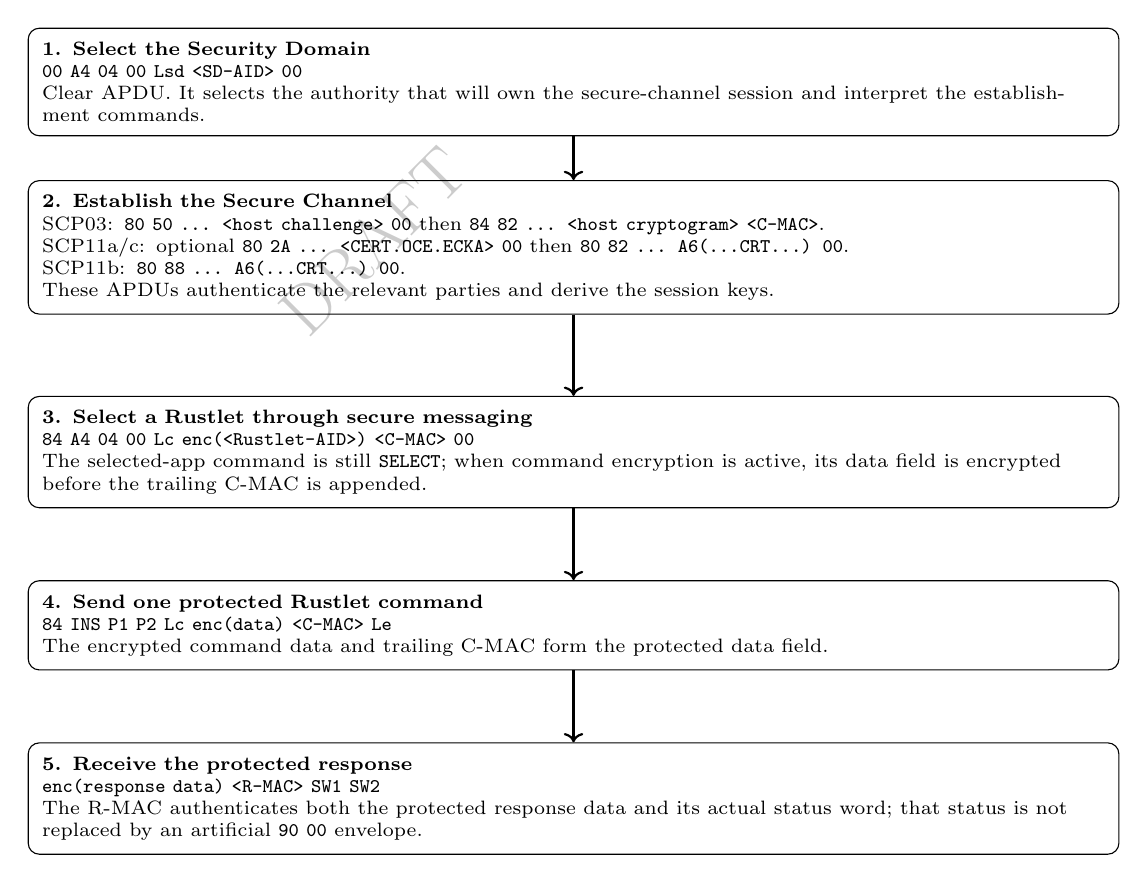
\begin{tikzpicture}[
    font=\scriptsize,
    scstep/.style={draw, rounded corners, align=left, text width=13.5cm,
                   inner sep=5pt},
    arrow/.style={->, thick}
]
\node[scstep] (s1) at (0,0) {
\textbf{1. Select the Security Domain}\\
\texttt{00 A4 04 00 Lsd <SD-AID> 00}\\
Clear APDU. It selects the authority that will own the secure-channel
session and interpret the establishment commands.
};

\node[scstep] (s2) at (0,-2.1) {
\textbf{2. Establish the Secure Channel}\\
SCP03: \texttt{80 50 ... <host challenge> 00}
then \texttt{84 82 ... <host cryptogram> <C-MAC>}.\\
SCP11a/c: optional \texttt{80 2A ... <CERT.OCE.ECKA> 00}
then \texttt{80 82 ... A6(...CRT...) 00}.\\
SCP11b: \texttt{80 88 ... A6(...CRT...) 00}.\\
These APDUs authenticate the relevant parties and derive the session keys.
};

\node[scstep] (s3) at (0,-4.7) {
\textbf{3. Select a Rustlet through secure messaging}\\
\texttt{84 A4 04 00 Lc enc(<Rustlet-AID>) <C-MAC> 00}\\
The selected-app command is still \texttt{SELECT}; when command encryption is
active, its data field is encrypted before the trailing C-MAC is appended.
};

\node[scstep] (s4) at (0,-6.9) {
\textbf{4. Send one protected Rustlet command}\\
\texttt{84 INS P1 P2 Lc enc(data) <C-MAC> Le}\\
The encrypted command data and trailing C-MAC form the protected data field.
};

\node[scstep] (s5) at (0,-9.1) {
\textbf{5. Receive the protected response}\\
\texttt{enc(response data) <R-MAC> SW1 SW2}\\
The R-MAC authenticates both the protected response data and its actual status
word; that status is not replaced by an artificial \texttt{90 00} envelope.
};

\draw[arrow] (s1) -- (s2);
\draw[arrow] (s2) -- (s3);
\draw[arrow] (s3) -- (s4);
\draw[arrow] (s4) -- (s5);
\end{tikzpicture}
\caption{Typical APDU flow from Security Domain selection to protected Rustlet command}
\label{fig:protected-rustlet-flow}
\end{figure}

%--------------------------------------------------
\subsection{CLA Encoding and Secure Messaging Indication}

The use of secure messaging is indicated directly in the APDU header, through
specific bits in the \texttt{CLA} byte.

In GlobalPlatform, the class byte encodes both:
\begin{itemize}
\item the logical channel number
\item the secure messaging status
\end{itemize}

When secure messaging is active, the \texttt{CLA} byte is modified to signal
that the APDU is protected. This affects how the command is interpreted by the
card:
\begin{itemize}
\item the payload must be unwrapped before processing
\item the MAC must be verified
\item the session state must be valid
\end{itemize}

This design ensures that secure messaging is orthogonal to the command
semantics: the same command (e.g., \texttt{INSTALL}) may be sent in clear or in
protected form, depending on the session state.

The exact encoding of secure messaging indicators within the \texttt{CLA} byte
is defined in the specification and must be handled consistently with logical
channel encoding \gpref{gp-card}{§9.4} \gpref{scp03}{§7}.

%--------------------------------------------------
\subsection{Operational Flow}

From a system perspective, the use of a Secure Channel follows a structured
sequence:

\begin{enumerate}
\item The host initiates the session using the protocol-specific establishment
      commands
\item The host authenticates using the protocol-specific authentication
      command(s)
\item The Secure Channel is established
\item Subsequent APDUs are transformed according to the common GlobalPlatform
      secure-messaging rules
\item The session remains active until explicitly terminated or reset
\end{enumerate}

This flow introduces a stateful layer on top of the APDU model, where the
interpretation of commands depends not only on their content but also on the
current session state.

\subsection{Protocol Invariants}

A conforming Secure Channel processing path must preserve the following
protocol invariants:

\begin{itemize}
\item session state is scoped to the selected Security Domain and logical
      channel;
\item session keys are used only within the session that derived them;
\item secure-messaging policy is enforced before command dispatch;
\item malformed protected APDUs, invalid MAC chains, stale receipts and replayed
      commands are rejected before their logical command is executed;
\item session invalidation prevents further use of the old MAC chain or old
      receipt material.
\end{itemize}

The implementation mapping of these invariants is described in Chapter~8
(Reference Implementation), Section~\ref{sec:impl-scp}.

\subsection{APDU Transformation under Secure Messaging}

Once the Secure Channel is established, APDU commands are no longer transmitted
in clear.  Instead, they are transformed through a wrapping process that
applies authentication and optional encryption to the command and response.

At a high level, the transformation operates as follows:
\begin{itemize}
\item the \texttt{CLA} byte is modified to indicate secure messaging
\item command data is optionally encrypted and the C-MAC is appended directly
      to the resulting data field
\item response data is optionally encrypted and the R-MAC is appended directly
      to it, before the actual \texttt{SW1/SW2}
\end{itemize}

This transformation preserves the logical structure of the APDU while modifying
its encoding and interpretation.
The precise binary ordering, padding, chaining and response-body shapes are
specified in Appendix~\ref{app:scp-data-objects}.

%--------------------------------------------------
\section{Secure Channel Extensions}

While Secure Channel Protocols define the core mechanisms required to protect
command APDUs, GlobalPlatform also specifies a set of extensions that enhance
the security model, in particular for response protection and advanced
messaging scenarios.

These extensions are not always mandatory but may be required depending on the
security policy of the deployment. At protocol level, they introduce additional
state and sequencing constraints that must be handled consistently with the
base SCP model.

%--------------------------------------------------
\subsection{Response Protection (R-MAC)}

The standard secure messaging model ensures the integrity and authenticity of
command APDUs.  However, responses returned by the secure element are not always
protected by default.

To address this limitation, GlobalPlatform defines a response protection
mechanism based on a Response Message Authentication Code (R-MAC). When
enabled, each response APDU includes a cryptographic MAC computed by the secure element
using the session key \texttt{S-RMAC} \gpref{scp03}{§6.2}.

This mechanism provides:
\begin{itemize}
\item integrity of response data
\item authentication of the secure element
\item protection against replay or modification of responses
\end{itemize}

Using R-MAC requires:
\begin{itemize}
\item maintaining a response MAC chaining state
\item computing and appending a MAC to each response
\item verifying this MAC on the host side
\end{itemize}

The detailed implementation of response MAC computation and verification is
described in Chapter~8 (Reference Implementation), Section~\ref{sec:impl-scp}.

\subsection{R-MAC Session Management}
\label{sec:rmac-session-management}

GlobalPlatform defines optional SCP03 commands to explicitly control the use
of response protection through R-MAC sessions. They are companion commands,
not part of the mandatory two-command SCP03 establishment sequence. SCP11 does
not support \texttt{BEGIN R-MAC SESSION} or \texttt{END R-MAC SESSION};
its response protection is selected directly by the key-usage qualifier in
the establishment CRT.

\apdudesc
{80}
{7A}
{00}
{00}
{00}
{00}
{none}
{none}

The \texttt{BEGIN R-MAC SESSION} command enables response protection for
subsequent APDUs.  Once activated, all responses returned by the secure element include
an R-MAC computed using the session key.

The command does not carry any payload and simply updates the session state.

On success, the secure element returns \texttt{90 00}. Failure may indicate:
\begin{itemize}
\item \texttt{6985}: conditions not satisfied
\item \texttt{6982}: security status not satisfied
\end{itemize}

\apdudesc
{80}
{78}
{00}
{00}
{00}
{00}
{none}
{none}

The \texttt{END R-MAC SESSION} command disables response protection.

After this command, response APDUs are no longer protected by an R-MAC,
although command protection (C-MAC, C-ENC) may still be active depending on the
session configuration.

This command restores a lighter communication mode while preserving the
established Secure Channel.

On success, the secure element returns \texttt{90 00}. Errors may include:
\begin{itemize}
\item \texttt{6985}: conditions not satisfied
\end{itemize}

\subsection{Secure Messaging Variants}

SCP03 supports multiple security levels that define how APDUs are protected.

These levels include:
\begin{itemize}
\item no protection
\item command authentication (C-MAC)
\item command authentication and encryption (C-MAC + C-ENC)
\item full protection including response authentication (R-MAC)
\end{itemize}

The selected security level is negotiated during the 
\texttt{EXTERNAL AUTHENTICATE} command and applies to all subsequent APDUs.

At protocol level, this implies that the APDU processing pipeline must be
capable of:
\begin{itemize}
\item selectively applying encryption
\item computing MACs
\item validating incoming MACs
\item handling different combinations of protection
\end{itemize}

This flexibility introduces additional complexity in the implementation, as all
combinations must be supported consistently.

\subsection{SCP Variants}

Several Secure Channel Protocol variants exist within GlobalPlatform, notably
SCP02 and SCP03.

SCP02 is based on legacy cryptographic primitives (DES/3DES), while SCP03
relies on AES and provides stronger security guarantees.

SCP03 is preferable to legacy DES-based SCP variants due to:
\begin{itemize}
\item improved security (AES-based)
\item simpler key derivation model
\item better resistance to known attacks
\end{itemize}

Supporting multiple SCP variants may be required for compatibility, but it
increases the protocol and certification surface. This document treats SCP03
and the SCP11 family as the reference profiles for the platform model.

%--------------------------------------------------
\subsection{Asymmetric and Post-Quantum Perspective}

Because the broader GlobalPlatform environment also handles certificates,
asymmetric keys, and delegated management artifacts, it is natural to ask
whether an SCP03 implementation must also embed asymmetric cryptography. The
answer is no: SCP03 itself does not require RSA, ECC, or post-quantum
asymmetric primitives. Its secure-channel core is fully symmetric and AES-based
\gpref{scp03}{§4, §6}.

This does not mean that asymmetric cryptography is irrelevant to the platform
as a whole. It means only that it belongs to other services: key transport
policies, certificate handling, platform attestation, application-specific
crypto services, or future secure-channel evolution. GlobalPlatform's own
discussion of crypto agility and hybrid migration highlights this distinction:
the current SCP03 core remains symmetric, while later evolutions may combine it
with stronger or more agile asymmetric layers \cite{gp-hybrid-crypto}.

If this project later introduces a minimal post-quantum asymmetric toolbox at
platform level, the most natural reference points are the NIST standards:
\begin{itemize}
\item ML-KEM for key encapsulation and shared-secret establishment
      \cite{fips203}
\item ML-DSA for general-purpose digital signatures \cite{fips204}
\item SLH-DSA as a stateless hash-based signature alternative \cite{fips205}
\end{itemize}

These algorithms are not required to implement SCP03. They should be viewed as
optional higher-level capabilities, introduced only if the platform later needs
public-key exchange, signatures, attestation, or hybrid migration strategies.
If such support is added, the dependency chain should also account for the
underlying SHA-3 and SHAKE primitives standardized by NIST \cite{fips202}.

%--------------------------------------------------
\section{oXiDe SE Beta Protocol Scope}
\label{sec:oxide-beta-protocol-scope}

The preceding sections state the protocol model against which oXiDe SE is
assessed. They must not be read as a claim that every optional GlobalPlatform
mechanism is already implemented. The beta reference implementation currently
supports short APDUs using its serial-line adaptation of \texttt{T=0}, the management-command subset
needed for Rustlet deployment and registry administration, SCP03 S8/S16 at
security levels \texttt{01} and \texttt{03} in the kernel-native Security
Domain, response-protecting SCP03 in the full Rustlet Security Domain, and the
implemented SCP11a, SCP11b, and SCP11c profiles.

The following mechanisms are deliberately outside the beta profile:
\begin{itemize}
\item legacy DES/TDEA-based SCP variants, including SCP02;
\item the optional SCP03 \texttt{BEGIN R-MAC SESSION} and
      \texttt{END R-MAC SESSION} commands;
\item SCP03 security levels \texttt{11}, \texttt{13}, and \texttt{33} in the
      deliberately smaller kernel-native Security Domain profile. The full
      Rustlet Security Domain provides the response-protecting path used by the
      beta test campaign.
\end{itemize}

Other mechanisms remain planned or incomplete rather than excluded from the
architecture. In particular, logical channels and \texttt{MANAGE CHANNEL} are
post-beta work. The beta also accepts only the management encodings exercised
by its declared profile: one complete BER-TLV object per \texttt{STORE DATA} command;
\texttt{INSTALL [for load]} and combined \texttt{INSTALL [for install and make
selectable]} with an empty token field; one final \texttt{PUT KEY} command with
the supported raw key types; and the documented registry/lifecycle subset.
Multi-command key updates, non-empty Tokens, DAPs, Receipts, key
diversification or wrapping, and the remaining optional management forms are
not yet implemented. Their absence is an implementation limitation, not a
reinterpretation of the commands defined by GlobalPlatform.

%--------------------------------------------------
\section{Discussion}

The previous sections introduced the communication model of a
GlobalPlatform-like environment by separating three concerns: the APDU
transport abstraction, the command semantics defined by the GlobalPlatform
instruction set, and the security layer provided by the Secure Channel
Protocol.

From an architectural perspective, this separation is not only conceptual but
directly maps to a software design. The platform can be understood as a system
that receives commands, interprets them according to its current state, and
produces responses. At the highest level, it behaves as a reactive system
driven by APDU inputs and generating APDU outputs.

\paragraph{A Layered Interpretation Model}

The processing of a command can be decomposed into three successive stages:

\begin{itemize}
\item \textbf{Transport layer (APDU parsing)}: decoding the structure of the
    incoming command (CLA, INS, P1, P2, payload), including logical channel
        routing.

\item \textbf{Security layer (SCP processing)}: verifying and removing secure
    messaging protection (MAC verification, decryption), and enforcing session
        validity.

\item \textbf{Semantic layer (command execution)}: interpreting the instruction
    and modifying the internal state of the platform accordingly.
\end{itemize}

These layers define a processing pipeline in which each stage transforms the
command before passing it to the next one. The reverse pipeline is applied when
constructing the response.

The detailed implementation of this pipeline is described in Chapter~8
(Reference Implementation), Sections~\ref{sec:impl-apdu-dispatch} and
\ref{sec:impl-scp}.

\paragraph{A State Machine View}

From the outside, the platform can be modeled as a state machine. Each incoming
APDU represents a transition request, whose validity and effect depend on the
current state of the system.

This state includes:
\begin{itemize}
\item the lifecycle state of managed objects (applications, load files,
    Security Domains)
\item the current selection context (logical channel and selected application)
\item the secure channel state (inactive, initialized, authenticated)
\end{itemize}

Commands such as \texttt{LOAD}, \texttt{INSTALL} or \texttt{SET STATUS} trigger
state transitions, while commands such as \texttt{GET STATUS} expose the
current state without modifying it.

The definition of managed objects and their lifecycle is provided in
Chapter~3, Sections~\ref{sec:gp-object-model} and \ref{sec:gp-lifecycle-model}.

\paragraph{An Interpreter Loop Perspective}

From the inside, the platform is naturally implemented as an interpreter loop:

\begin{enumerate}
\item receive an APDU command
\item parse and validate its structure
\item unwrap secure messaging if required
\item dispatch the command based on its instruction code
\item execute the corresponding handler
\item produce a response APDU
\item apply secure messaging to the response if required
\item return the response
\end{enumerate}

This loop provides a unifying view of the system, where each command is treated
as an instruction in a control interface. The GlobalPlatform command set can
thus be interpreted as a minimal instruction set driving the evolution of the
platform state.

The implementation of this interpreter loop is detailed in Chapter~8 (Reference
Implementation).

\paragraph{Freedom of Implementation}

An important property of the GlobalPlatform model is that it defines a protocol
of interaction rather than an execution model. In particular:

\begin{itemize}
\item the format of application binaries is not specified
\item the runtime environment is not constrained
\item the internal representation of objects is implementation-dependent
\end{itemize}

This leaves significant freedom to the implementer, while ensuring
interoperability at the protocol level. As a result, different platforms may
expose identical command interfaces while relying on very different internal
architectures.

\paragraph{Link with the Threat Model}

The architecture described above directly relates to the threat model
introduced earlier.  Each layer of the processing pipeline corresponds to a
security boundary:

\begin{itemize}
\item the APDU interface is exposed to external adversaries
\item the secure channel enforces authenticity and integrity of commands
\item the command execution layer must enforce isolation and lifecycle
    constraints
\end{itemize}

In particular, the interpreter loop must ensure that:
\begin{itemize}
\item no command can bypass security checks
\item malformed or malicious inputs are rejected early
\item state transitions remain consistent with the lifecycle model
\end{itemize}

This highlights the importance of a strict separation between parsing, security
enforcement and command execution, as well as the need for explicit validation
at each stage.

From this perspective, the GlobalPlatform model can be seen as a controlled
interface to a stateful system, where security relies on the correct
composition of protocol handling, cryptographic protection and state
management.

\chapter{GlobalPlatform Object and Administration Model}

This chapter defines the object, authority, and lifecycle model against which
oXiDe SE is designed. Chapter~3 introduced the protocol vocabulary---APDUs,
GlobalPlatform commands, selection, and Secure Channels. The present chapter
answers the corresponding stateful questions: \emph{which resident entities
are addressed by those commands, how are they related, and under whose
authority may they be managed?}

Three kinds of statement are kept distinct throughout the chapter:

\begin{description}
\item[GlobalPlatform reference model.] These paragraphs summarize the
      concepts and command semantics defined by the GlobalPlatform Card
      Specification.
\item[oXiDe SE implementation contract.] These paragraphs state the
      architecture and invariants that an oXiDe SE implementation is expected
      to enforce. They are design requirements, not claims of formal proof.
\item[Beta implementation status.] These paragraphs identify the implemented
      subset and the remaining validation or implementation work. Detailed
      mechanisms and evidence are deferred to the implementation and test
      chapters.
\end{description}

This separation is important. Compatibility with the GlobalPlatform object
model does not require oXiDe SE to reproduce every optional management mode,
and an internal oXiDe SE representation must not be mistaken for a structure
mandated by GlobalPlatform.

%--------------------------------------------------
\section{Platform Object Model}
\label{sec:gp-object-model}

% Plan:
% - define the main GP-managed entities
% - explain that AIDs are the stable identifiers used by registry and dispatch
% - distinguish executable content, installed instances, and security authorities
% - introduce the registry view as the structured catalog of those entities

\subsection{GlobalPlatform Reference Entities}

GlobalPlatform does not begin from a process model or an operating-system
abstraction. It begins from managed entities resident on the secure element
and from the relationships between them. The principal reference entities are
\gpref{gp-card}{§7, §9, §11}:

\begin{itemize}
\item an \textbf{Executable Load File}, which represents deployable code
  transported to the secure element through the loading protocol;
\item an \textbf{Executable Module}, which identifies installable code within
  an Executable Load File;
\item an \textbf{Application}, or more precisely an installed application
  instance, which may later be selected and addressed through APDUs;
\item a \textbf{Security Domain}, which is also an application-like
  resident entity but with management responsibilities, privileges, and
  associated cryptographic material;
\item the unique \textbf{Issuer Security Domain} of one GlobalPlatform
  environment, which is the first application and has the special role
  defined by the Card Specification.
\end{itemize}

These entities are not merely names in a registry. They are the objects
whose lifecycle is controlled by commands such as \texttt{LOAD},
\texttt{INSTALL}, \texttt{DELETE}, \texttt{SET STATUS}, and
\texttt{GET STATUS}. The command vocabulary introduced in Chapter~3
therefore only becomes meaningful once these entities have been
distinguished.

Conceptually, the \textbf{GlobalPlatform Registry} is the organized view of
the managed world inside the secure element. It records which load files,
modules, applications, and Security Domains exist, how they are associated,
and which privileges and lifecycle states apply. Security-Domain keys and data
belong to the administrative model, but representing each key as an
AID-addressable registry object is not required by GlobalPlatform.

\subsection{oXiDe SE Managed Objects}

oXiDe SE implements one persistent registry containing packages, Rustlet
instances, Security Domain instances, key objects, and generic data objects.
Using the same bounded representation for these families is an oXiDe SE design
choice. It permits the same ownership, persistence, lifecycle, and deletion
rules to be applied consistently, while command handlers retain the distinct
GlobalPlatform semantics of each object family.

One oXiDe package record represents one FAE Executable Load File and records
the single Executable Module AID from which its Rustlet instances may be
created. Executable Modules are therefore projected in \texttt{GET STATUS},
but are not independently stored or lifecycle-managed registry entries. A
multi-module Executable Load File is outside the beta model.

Every managed object is attached to an administrative Security Domain. The
internal field \path{parent_sd_aid} records that containment relation. One
exception is structural: the oXiDe Root Security Domain has no parent and is
the unique root of the internal registry tree. This root is an oXiDe SE
platform entity; it is not necessarily the GlobalPlatform Issuer Security
Domain.

%--------------------------------------------------
\subsection{Object Identification}
\label{sec:gp-object-identification}

% Plan:
% - explain AIDs as the primary GP identifiers
% - distinguish load-file AID, application-instance AID, and security-domain AID
% - state uniqueness and role in selection, management, and registry references

The primary identifier used throughout GlobalPlatform is the
\textbf{Application Identifier} (AID). Even though the name comes from
ISO/IEC~7816 and from the application-selection model, GlobalPlatform
uses AIDs more broadly: an AID identifies not only a selectable
application instance, but also Security Domains and load-file-related
objects referenced by management commands \gpref{gp-card}{§7, §11}.

Several distinct AIDs may therefore coexist for conceptually related
objects:

\begin{itemize}
\item an \textbf{Executable Load File AID} identifies the executable content being
  transported and installed;
\item an \textbf{Application AID} identifies an installed instance that
  may later become selectable;
\item a \textbf{Security Domain AID} identifies the administrative
  entity under whose authority management actions are performed.
\end{itemize}

This distinction matters because GlobalPlatform deliberately separates
deployable code, installed instances, and administrative authority. A
single load file may give rise to one or more installed instances, and
those instances may later be placed under the responsibility of a given
Security Domain. The identifiers must therefore remain stable across
management operations and allow those relationships to be expressed
explicitly.

From a protocol perspective, AIDs are also the bridge between the APDU
world and the object model. They appear in \texttt{SELECT}, in
\texttt{INSTALL} parameters, in registry-oriented queries, and in
administrative operations such as deletion or lifecycle updates. An AID
is therefore not just a name looked up at selection time; it is the
stable handle by which GlobalPlatform refers to a managed secure-element
entity across
its whole management model.

For an off-card operator, a minimal useful set of identifiers is
therefore:
\begin{itemize}
\item the AID of the oXiDe Root Security Domain when a platform-wide
  administration operation is intentionally requested;
\item the AID of the Issuer Security Domain, when one is present, which is the
  usual entry point for secure-element administration;
\item the AID of any supplementary Security Domain used for delegated or
  specialized administration;
\item the AID of the target application instance to be selected or
  personalized;
\item the AID of the corresponding load file when deployment or removal
  operations are performed.
\end{itemize}

The Root Security Domain AID and an Issuer Security Domain AID designate
different roles even when a particular configuration chooses the same backend
implementation for both. The former selects the oXiDe SE platform root; the
latter, when declared, selects the unique Issuer Security Domain of the
GlobalPlatform environment.

%--------------------------------------------------
\subsection{Object Relationships}
\label{sec:gp-object-relationships}

% Plan:
% - explain dependency graph between load files, apps, and security domains
% - explain associated security-domain relationship
% - introduce the idea that management invariants arise from these relations

The GlobalPlatform object model is relational rather than flat. The most
important relationships are:

\begin{itemize}
\item an installed application instance depends on executable content
  that was previously made present on the secure element through the loading
  process;
\item an application instance is associated with a Security Domain that
  acts as its administrative authority;
\item a Security Domain owns keys, privileges, and management authority
  that are distinct from the application business logic itself.
\end{itemize}

These relationships are not optional conceptual decorations. They are
what gives management commands their preconditions and their effects. An
application cannot be installed if the relevant executable content is not
present; a simple load-file deletion cannot proceed while installed instances
still depend on it, whereas cumulative deletion explicitly includes related
objects; a sensitive management action is interpreted under the authority
of a Security Domain rather than under the identity of an arbitrary
selected application.

\subsection{GlobalPlatform Association Forest}

GlobalPlatform associates each Application and Executable Load File with a
Security Domain. Because a Security Domain is itself an Application, Security
Domains may form association hierarchies. The Issuer Security Domain is
effectively associated with itself. GlobalPlatform also permits another
Security Domain to become self-associated through extradition, thereby forming
the root of another association hierarchy \gpref{gp-card}{§7.1, §7.2}.

There is no contradiction between one Issuer Security Domain and several
association hierarchies. Only one root has the special Issuer Security Domain
role. Other self-associated roots remain supplementary Security Domains. Their
providers may use distinct keys and administer content independently of the
Card Issuer's ordinary management context.

The GlobalPlatform association model is therefore a forest. Its usual shape
has the Issuer Security Domain at the root of the principal hierarchy, with
most supplementary Security Domains below it. Additional self-associated
Security Domains may head detached hierarchies.

\subsection{oXiDe SE Internal Root and Tree Projection}

oXiDe SE represents that forest as one internal tree by adding a unique
technical root:

\begin{verbatim}
oXiDe Root Security Domain
|-- Issuer Security Domain
|   |-- ordinary Security Domain A
|   `-- ordinary Security Domain B
`-- detached Security Domain C
    `-- ordinary Security Domain C.1
\end{verbatim}

In a production-oriented composition, at least the oXiDe Root Security Domain
and the Issuer Security Domain are normally pre-deployed. The Issuer Security
Domain is explicitly marked as such and is a direct child of the root;
ordinary Security Domains are normally attached to the Issuer Security Domain
or one of its descendants. A GlobalPlatform hierarchy detached from the Issuer
hierarchy is represented internally by attaching its self-associated root
directly to the oXiDe root. Development compositions may deliberately declare
only the technical root and therefore have no distinct Issuer Security Domain.

The first internal edge has a different interpretation from an ordinary
GlobalPlatform association. In the GlobalPlatform-facing projection, the
Issuer Security Domain and every detached hierarchy root are self-associated.
Their internal parent is the oXiDe root only for platform containment,
visibility, persistence, and recovery. Registry responses must preserve this
distinction and must not accidentally expose the technical root as the
GlobalPlatform associated Security Domain of those roots.

\subsection{Uniform Subtree Visibility}

oXiDe SE gives the internal tree one uniform operational interpretation. A
Security Domain may resolve its own objects and every object contained in its
descendant Security Domains. It cannot resolve objects owned by an ancestor or
by a sibling branch. Objects outside that view are treated as absent for the
administrative operation, which avoids disclosing their existence.

For every Security Domain $S$, let $V(S)$ be its visible registry set. If $C$
is a child of $P$, the structural invariant is:

\begin{center}
$V(C) \subseteq V(P)$.
\end{center}

The root's descendants are all managed objects, so $V(root)$ is the complete
registry. The Issuer Security Domain sees the usual Issuer hierarchy but not a
detached root or its descendants. Two detached hierarchies are mutually
invisible. A newly created object is attached to the active Security Domain
that authorizes its creation. In the beta, detached hierarchy roots may be
declared by predeployment beneath the technical root; post-issuance
extradition and reattachment are not implemented.

Visibility is necessary but not sufficient for authorization. Command type,
delegated privileges, Secure Channel state, lifecycle, dependency checks, and
the selected Security Domain's own policy remain mandatory after lookup.

\subsection{Uniform Authority and Monotone Delegation}
\label{sec:gp-privilege-delegation}

When this chapter speaks about Security-Domain ``rights'', it does not mean
ordinary application permissions. It means GlobalPlatform administrative
privileges: the authority to perform families of management operations on
resident objects. Examples include loading executable content, installing an
application instance, deleting managed objects, changing lifecycle state,
managing secure-channel keys, performing delegated management, requesting or
verifying deployment tokens, generating receipts, or exercising card-level
lock and termination operations.

These privileges are attached to Security Domain instances. An ordinary
application instance does not become a management authority merely because it
lives under a privileged Security Domain. It is administered by that Security
Domain, and it may rely on services made available through that association,
but registry mutation and platform administration remain Security-Domain
authority.

GlobalPlatform defines specialized privileges whose roles are not, by
themselves, a simple parent-to-child lattice. oXiDe SE deliberately imposes a
stricter and more uniform rule: a Security Domain may delegate only authority
that it already possesses, and a child must not receive a broader privilege
set than its parent. If $R(S)$ denotes the operations granted to $S$, then:

\begin{center}
$R(C) \subseteq R(P)$.
\end{center}

Combined with subtree visibility, this gives
$V(C) \subseteq V(P)$ and $R(C) \subseteq R(P)$. Administrative delegation
may restrict or subdivide authority; it cannot amplify either its operations
or its reach.

GlobalPlatform's \emph{Global Delete}, \emph{Global Lock}, and
\emph{Global Registry} are privileges, not distinct instruction bytes. In the
reference model, an Application or Security Domain holding the corresponding
privilege may act independently of ordinary Security-Domain association or
hierarchy restrictions \gpref{gp-card}{§9.1.3.4--§9.1.3.5, §9.6.5}.

oXiDe SE intentionally adopts a narrower beta contract. Only the technical
root obtains transverse reach, as a consequence of being the ancestor of every
internal hierarchy. A non-root Security Domain never escapes its subtree, even
if its stored privilege bytes contain a Global Delete, Global Lock, or Global
Registry bit. The common mutation and query primitives remain parameterized by
an authority AID; invoking them with the root AID gives them complete reach
without bypassing registry, lifecycle, persistence, or dependency checks. This
is an explicit oXiDe SE profile restriction relative to the GlobalPlatform
privilege semantics, not a restatement of the standard.

%--------------------------------------------------
\subsection{Selected Context and Visible Endpoints}
\label{sec:gp-selected-context}

% Plan:
% - explain what a host actually addresses when talking to the card
% - distinguish selected Security Domain and selected ordinary application
% - connect this to Chapter 3 without entering kernel design

From the point of view of an external management tool, the secure
element does not expose a single flat command receiver. It exposes a set
of \textbf{selectable contexts}. Through \texttt{SELECT}, the off-card
entity chooses which AID becomes the current communication endpoint. Four
situations matter most:

\begin{itemize}
\item the \textbf{oXiDe Root Security Domain} is selected for an explicitly
  platform-wide operation. Its ordinary subtree is the complete registry;
\item a \textbf{Security Domain} is selected, typically the Issuer
  Security Domain, and subsequent commands are interpreted in the
  administrative plane of the secure element;
\item an \textbf{ordinary application} is selected, and subsequent
  commands are interpreted according to that application's own semantics;
\item no application-specific management action is possible until the
  appropriate administrative context has first been selected.
\end{itemize}

This explains an important operational distinction already hinted at in
Chapter~3. Commands such as \texttt{LOAD}, \texttt{INSTALL},
\texttt{DELETE}, \texttt{PUT KEY}, \texttt{GET STATUS}, or
\texttt{INITIALIZE UPDATE} are not merely generic APDU opcodes that can
be sent to any selected endpoint. They are meaningful only in the
appropriate administrative context, i.e. under a Security Domain
authorized to interpret them.

In oXiDe SE this authorization is not modeled as a collection of
independent ad hoc checks spread across the kernel. The object registry is
also the visibility boundary for the resolved administrative authority. A
lookup under one Security Domain resolves only within the subtree
administratively reachable from that Security Domain. An object outside this
visible subtree is treated as absent in that context. This design makes the
management rule above mechanically enforceable: the resolved authority may
act on its own objects and on objects of its descendants, while new objects
are created under that authority.

The beta resolves that authority differently for its two supported development
paths. A protected management APDU is bound to the active Security Domain and
its Secure Channel. A clear management APDU is bound to the technical root and
is accepted only by a permissive root backend such as
\texttt{NullSecurityDomain}. Selecting a child Security Domain does not make
clear management APDUs execute under that child. Logical-channel-specific
selection and Secure Channel contexts remain future work.

Conversely, once an application instance has been selected, the same APDU
transport is used, but the semantics changes entirely: the secure element
interprets the APDU according to the application contract rather than
according to the GlobalPlatform administration model.

%--------------------------------------------------
\section{Lifecycle Model}
\label{sec:gp-lifecycle-model}

% Plan:
% - define lifecycle as state machine over GP objects
% - explain that transitions are command-driven and constrained
% - prepare the object-specific lifecycle subsections

GlobalPlatform associates lifecycle states with the principal managed
objects on the secure element. A lifecycle state is more than a diagnostic label:
it controls what operations are currently permitted on a given entity and
which command sequences remain legal \gpref{gp-card}{§9.6, §11}.

Conceptually, the lifecycle model combines three ideas:

\begin{itemize}
\item a managed object is always in a well-defined state;
\item only certain transitions are allowed from a given state;
\item commands such as \texttt{INSTALL}, \texttt{SET STATUS},
  \texttt{DELETE}, and \texttt{SELECT} are interpreted against that
  state machine rather than in isolation.
\end{itemize}

This is why administration and deployment cannot be described purely as a
list of commands. They are organized as stateful workflows. A load-file
transfer, an application installation, a personalization session, or a
deletion sequence only make sense because the addressed object moves
through allowed states and because invalid transitions are rejected.

For a security specialist using the secure element, the practical consequence is
that the current state of the addressed object is always part of the
precondition of a command. A management script therefore needs more than
an AID and an opcode: it needs a correct view of whether the target load
file is present, whether the application instance already exists, whether
it is selectable, and whether the selected Security Domain is currently
allowed to perform the requested transition.

GlobalPlatform defines object-specific lifecycle models
\gpref{gp-card}{§5.2--§5.3}. An Executable Load File has only the
\texttt{LOADED} state. An ordinary Application has \texttt{INSTALLED},
\texttt{SELECTABLE}, and \texttt{LOCKED} states, plus any application-specific
states. A supplementary Security Domain has \texttt{INSTALLED},
\texttt{SELECTABLE}, \texttt{PERSONALIZED}, and \texttt{LOCKED} states. The
Issuer Security Domain instead inherits the Card Life Cycle State. The
following subsections do not replace those definitions. They describe the
deliberately smaller and partly implementation-specific projection used by the
oXiDe SE beta registry.

Absence, deletion, and failed installation are represented by the absence of a
committed registry entry, not by an additional lifecycle value. oXiDe SE uses
one compact state pair per ordinary managed-object family:

\begin{center}
\begin{tabular}{p{0.22\textwidth}p{0.22\textwidth}p{0.42\textwidth}}
\textbf{Object family} & \textbf{States} & \textbf{Operational guard} \\
\hline
\texttt{Package} & \texttt{Loaded}, \texttt{Locked} &
  only \texttt{Loaded} packages may be instantiated; \texttt{Locked} is an
  oXiDe extension, not a GlobalPlatform Executable Load File state; \\
\texttt{Instance} & \texttt{Selectable}, \texttt{Locked} &
  only \texttt{Selectable} instances may be selected; \\
\texttt{SecurityDomain} & \texttt{Selectable}, \texttt{Locked} &
  only \texttt{Selectable} Security Domains may be selected or used to open a
  secure channel; \\
\texttt{Key} & \texttt{Active}, \texttt{Locked} &
  only \texttt{Active} keys may be used by secure-channel derivation; these are
  internal oXiDe states, not GlobalPlatform Registry lifecycle values.
\end{tabular}
\end{center}

The internal \texttt{Locked} state is conservative. It keeps the object
visible to management code, but prevents the operation that would normally
make the object effective: instantiating a package, selecting an instance,
opening a secure channel through a Security Domain, or deriving session keys
from a key object. The data model can represent all four locked forms, but the
current APDU surface does not expose all their transitions. Future profiles
may add richer state values, but those values are not part of the beta
lifecycle contract.

The oXiDe root is not an ordinary GlobalPlatform lifecycle object: it exists
from bootstrap, has no parent, and cannot be deleted or have its state changed
through the beta management APDUs. The Issuer Security Domain is also distinct
from an ordinary supplementary Security Domain because GlobalPlatform makes it
inherit the Card Life Cycle State. The beta registry nevertheless stores both
Issuer and supplementary Security Domains using the compact
\texttt{Selectable}/\texttt{Locked} pair. Card lifecycle and the complete
Issuer lifecycle projection are not implemented.

%--------------------------------------------------
\subsection{Application Lifecycle}
\label{sec:gp-lifecycle-application}

% Plan:
% - describe the conceptual lifecycle of an application instance
% - emphasize installation, selectability, locking, and administrative control
% - link conceptually to INSTALL / SET STATUS without implementation details

For an application instance, the retained lifecycle distinction is simple:
the instance is either selectable or locked. GlobalPlatform distinguishes
installation from the transition that makes an instance selectable. The beta
profile currently uses the combined \texttt{INSTALL [for install and make
selectable]} form and creates the instance directly in the
\texttt{Selectable} state when policy, package lookup, and the Rustlet
installation call all succeed. A failed installation does not create a stable
registry object.

The practical consequence is that \texttt{SELECT} is authorized by the
instance state. A \texttt{Selectable} instance may become the current
application context; a \texttt{Locked} instance remains known to management
code but cannot be selected. Deletion removes the registry entry and therefore
returns the instance to the operationally absent condition.

The normal application-instance transitions are:

\begin{itemize}
\item \textbf{absent to selectable}: caused in the beta profile by the
  successful combined install-and-make-selectable form of \texttt{INSTALL}.
\item \textbf{selectable to locked}: represented by the beta's restricted
  \texttt{SET STATUS} path or by kernel policy.
\item \textbf{locked to selectable}: represented by the same restricted
  path. The full GlobalPlatform status-type and previous-state rules are not
  yet implemented.
\item \textbf{selectable or locked to absent}: caused by \texttt{DELETE},
  provided dependency and privilege checks allow removal.
\end{itemize}

\texttt{SELECT} itself does not install an application and does not create a
new lifecycle state. It only makes an already selectable application the
current execution context. Conversely, deselection is a change of current
context, not a registry lifecycle transition.

%--------------------------------------------------
\subsection{Load File Lifecycle}
\label{sec:gp-lifecycle-loadfile}

% Plan:
% - explain load files as deployable content with their own lifecycle
% - distinguish load-file presence from application-instance usability
% - explain dependency constraints on removal

The lifecycle of executable content is different from that of application
instances. A package is first transported, validated and committed as executable
content. Its conceptual role is to make code available on the secure element so
that one or more application instances may later be installed from it.

This means that a load file may exist even when no currently selectable
application has yet been created from it, and conversely that an
installed application may continue to depend on that load file for as
long as the instance exists. The load-file lifecycle therefore captures
availability and dependency rather than direct selectability.

From a management perspective, this is what explains the asymmetry
between \texttt{LOAD} and \texttt{DELETE}. Loading introduces executable
content as a managed dependency; deletion must later respect the fact
that other objects may still rely on that content.

The oXiDe package transitions are:

\begin{itemize}
\item \textbf{absent to loaded}: caused by a complete and valid
  \texttt{INSTALL [for load]} plus \texttt{LOAD} sequence. The temporary load
  context is volatile until the final block has been checked; only the final
  success creates the package registry entry.
\item \textbf{loaded to locked}: caused by the beta's diagnostic
  \texttt{SET STATUS} extension or kernel policy. A locked package remains
  present but cannot be used by \texttt{INSTALL [for install]} to create a new
  instance. GlobalPlatform itself defines no \texttt{LOCKED} Executable Load
  File lifecycle state.
\item \textbf{locked to loaded}: caused by the corresponding oXiDe diagnostic
  unlock operation.
\item \textbf{loaded or locked to absent}: caused by a simple \texttt{DELETE}
  when no installed instance or dependent object still requires the load file,
  or by cumulative deletion that explicitly includes the related objects.
\end{itemize}

This model deliberately keeps partially received code outside the stable
registry. The registry must never advertise a load file as usable before the
whole binary has been received and validated.

%--------------------------------------------------
\subsection{Security Domain Lifecycle}
\label{sec:gp-lifecycle-domain}

% Plan:
% - explain that security domains also have lifecycle states
% - stress their administrative role and privileged status
% - distinguish them from ordinary applications without entering implementation

Security Domains also have lifecycle states, but their meaning is more
administrative than purely functional. A Security Domain is not only a
selectable entity; it is also a carrier of privileges, keys, and
management authority. As a result, its lifecycle constrains not only its
own reachability but also which administrative operations may lawfully be
performed under its authority.

Three cases must be distinguished in oXiDe SE. The Root Security Domain is the
non-deletable technical anchor and is outside ordinary Security Domain
lifecycle transitions. When present, the Issuer Security Domain is the unique
GlobalPlatform issuer endpoint and inherits the card lifecycle in the
GlobalPlatform reference model. Supplementary and detached Security Domains
are ordinary lifecycle-bearing administrative principals.

In many operational environments, the Issuer Security Domain is also the
administrative endpoint informally associated with the \emph{Card Manager}
role. In strict GlobalPlatform terminology, however, \emph{Card Manager} is a
broader historical label than \emph{Issuer Security Domain}. This document
therefore keeps \emph{Issuer Security Domain} as the precise preferred term for
the selected administrative endpoint with which an off-card management tool
first establishes trust and through which it performs secure-element-management
operations.

For an ordinary Security Domain, the compact beta transitions are:

\begin{itemize}
\item \textbf{absent to selectable}: caused by the successful combined
  install-and-make-selectable form of \texttt{INSTALL} when the instance is declared as a
  Security Domain. The command fixes the Security Domain instance AID, backend
  or package binding, initial administrative state, and base privilege bytes.
  Once selectable, the Security Domain may be selected as an administrative
  endpoint and may establish secure channels according to its key and profile
  policy.
\item \textbf{selectable to locked}: represented by the beta's restricted
  \texttt{SET STATUS} transition or by platform policy. A locked Security
  Domain remains a registry object, but it cannot be selected and cannot be
  used to establish a secure channel. Because secure-channel establishment is
  the entry point for protected management authority, this also prevents normal
  administrative use under that Security Domain.
\item \textbf{locked to selectable}: represented by the same restricted
  unlock path.
\item \textbf{selectable or locked to absent}: caused by simple
  \texttt{DELETE} when no descendants or key dependencies remain, or by an
  authorized cumulative deletion that includes the complete subordinate
  closure.
\end{itemize}

The key difference from ordinary application lifecycle is that Security Domain
state gates authority as well as selectability. A selectable application may
process application APDUs; a selectable Security Domain may additionally
authorize administrative operations, manage key material, and host secure
channel state. A locked Security Domain therefore does not merely become
unselectable: it also stops being a usable management authority.

The lifecycle returned through the standard lifecycle data object
\texttt{9F70} must reflect the effective state of the selected Security
Domain. In oXiDe SE terms, this is the state stored with the Security Domain
registry object or, for a Rustlet-backed Security Domain, the state reported by
the selected Rustlet Security Domain through its dedicated management
interface.

The current \texttt{SET STATUS} decoder is not yet a conformant implementation
of the GlobalPlatform state machine. GlobalPlatform uses P1 values to
distinguish the Issuer Security Domain, Applications or supplementary Security
Domains, and a Security Domain together with its associated Applications; P2
contains the requested standard lifecycle value
\gpref{gp-card}{§11.10}. The beta instead accepts an internal package category,
maps its three categories directly to package, application, and Security
Domain registry kinds, and accepts only compact lock/unlock controls. In
particular it neither implements the Issuer/Card Life Cycle State nor the
standard recursive Security-Domain-and-associated-Applications form. This path
is diagnostic functionality pending protocol realignment.

%--------------------------------------------------
\subsection{Key Object State}
\label{sec:gp-lifecycle-key}

GlobalPlatform associates key material and key-management operations with a
Security Domain, but it does not define the oXiDe key entries as ordinary
GlobalPlatform Registry objects with a common lifecycle. oXiDe nevertheless
stores typed key objects beneath their owning Security Domain. Their internal
state is orthogonal to key version, key identifier, usage, and raw material and
answers one operational question: may this key be used by secure-channel
establishment?

The current externally reachable behavior is:

\begin{itemize}
\item \textbf{absent to active}: caused by successful key provisioning, such
  as \texttt{PUT KEY}. The key object becomes available to the corresponding
  secure-channel profile.
\item \textbf{active to active}: a later \texttt{PUT KEY} may replace the
  matching owner-qualified key identity.
\end{itemize}

The registry representation also contains \texttt{Locked}, and secure-channel
lookup correctly ignores a key in that state, but no conformant management APDU
currently performs the Active/Locked transition. Generic deletion by the
synthetic internal key-object AID is an implementation facility, not a
GlobalPlatform key-removal interface. Key rotation does not require a separate
lifecycle state. Moreover, a multi-key \texttt{PUT KEY} is presently applied
and persisted entry by entry: complete key-set replacement is not atomic and a
late parsing or storage failure may leave earlier entries updated. This is a
beta limitation that must be removed before claiming complete
\texttt{PUT KEY} interoperability.

%--------------------------------------------------
\section{Deployment Workflow}
\label{sec:gp-deployment-workflow}

% Plan:
% - describe the canonical deployment flow at GP level
% - keep it conceptual, not implementation-specific
% - connect secure channel, load, install, personalization, and activation

At a conceptual level, GlobalPlatform deployment is a staged workflow
rather than a single command. A typical sequence is:

\begin{enumerate}
\item select the relevant Security Domain, typically the Issuer Security
  Domain;
\item establish the administrative authority and, when required, a
  secure channel through \texttt{INITIALIZE UPDATE} and
  \texttt{EXTERNAL AUTHENTICATE};
\item prepare the secure element for receiving executable content;
\item transfer that content through one or more \texttt{LOAD} commands;
\item create or configure the installed instance through one of the
  \texttt{INSTALL} variants;
\item optionally personalize the instance;
\item make it selectable or otherwise transition it to the intended
  operational state.
\end{enumerate}

In oXiDe SE, a Rustlet normally follows this workflow after issuance: its FAE
image is built independently, transferred to an already deployed secure
element, and installed under the authority of a Security Domain. For a
controlled initial image, oXiDe SE also supports pre-issuance deployment. The
build configuration then embeds the Rustlet and declares its package and
instance relationships in the predeployment manifest, so that they form part of
the initial registry. Predeployment changes when the content enters the system;
it does not turn the Rustlet into kernel code or bypass the managed-object,
authority, lifecycle, and isolation models described in this chapter.

\subsection{Bootstrap and the Initial Administrative Tree}

A production-oriented oXiDe SE image normally pre-deploys at least two distinct
administrative objects. The Root Security Domain establishes the technical
root, initial registry authority, and recovery context. The unique Security
Domain explicitly declared with \texttt{role = "issuer"}, when present, is a
direct child of that root and is the normal entry point for subsequent
card-content management. Other pre-deployed Security Domains are ordinarily
placed below the Issuer hierarchy. A Security Domain attached directly to the
oXiDe root is projected as the self-associated root of a detached
GlobalPlatform hierarchy.

This is one schema rather than a set of image profiles. A kernel-only image
uses only the materialized technical root and kernel APDU modules. A
Rustlet-development image declares a permissive root with no child Security
Domain. A Security-Domain test image adds whatever hierarchy it exercises. A
production-oriented hierarchy declares exactly one Issuer and the required
protected policies. Zero Issuer declarations therefore means that no distinct
Issuer exists; one identifies it; a second is rejected. The build validates
parents, cycles, duplicate AIDs, and monotone privileges, then materializes the
root, the optional Issuer, and the remaining domains in parent-before-child
order independently of TOML declaration order.

This bootstrap is part of the trusted initial image. Post-issuance management
cannot manufacture a second parentless object, replace the oXiDe root, or
change its lifecycle through the beta APDU surface. Dynamic extradition and
detachment are not implemented; detached roots are currently established only
by trusted predeployment.

This workflow explains why the same command vocabulary is reused in
different combinations. For example, \texttt{INSTALL} is not a single
one-dimensional action: its mode flags let it participate in loading,
installation, personalization, make-selectable, registry-update, or
extradition workflows. The command set is therefore best read as a
workflow language for secure-element administration.

At this stage, two operational points are worth making explicit.

First, management activity is usually embedded in an authenticated
session. In a secure deployment, an operator is not expected to send
\texttt{LOAD}, \texttt{INSTALL}, \texttt{PUT KEY}, or similar commands
as isolated cleartext APDUs. The normal pattern is to select the
administrative Security Domain, establish its configured Secure Channel---for
example SCP03 or an SCP11 variant---and only then execute the management
workflow.

Second, personalization is conceptually part of deployment, but it is not
the same thing as installation. Installation creates or configures the
instance; personalization transfers instance-specific data. This is why a
deployment sequence may remain incomplete, from the operational point of
view, even after the executable content has been loaded and the
application instance has been created.

The beta profile implements the Rustlet load/install path needed by its test
and development workflows, but not every GlobalPlatform personalization,
extradition, Token, DAP, or Receipt form described by the reference workflow.
Those omissions are implementation limits, not alternative definitions of the
GlobalPlatform operations.

\subsection{Hierarchy Removal and Cumulative Delete}

Deletion is evaluated by the same authority-and-visibility rule as creation or
update. A simple deletion removes one visible object only when doing so leaves
no live dependency. Deleting a package with installed instances, or deleting a
Security Domain that still owns objects or subordinate domains, must therefore
fail in the simple form.

Cumulative deletion changes the requested target set, not the authorization
model. GlobalPlatform~2.3.1 defines hierarchy or sub-hierarchy cumulative
deletion as an optional operation performed by a Security Domain with Global
Delete privilege \gpref{gp-card}{§9.5.3--§9.5.4}. The oXiDe beta applies a
narrower tree rule: an authority may request the cumulative form only over a
target and closure already contained in its own visible subtree; transverse
scope is obtained only by using the technical root.

The implementation first computes the complete related-object closure:
instances belonging to a package, or Security Domains and managed content in a
subordinate hierarchy. Every member must remain within the active authority's
visible subtree. The in-RAM entries are removed dependants first and the
resulting registry is published in one persistent snapshot. Flash recovery can
therefore retain the previous valid snapshot if publication is interrupted;
this does not claim a general transaction mechanism for arbitrary mutations.

The oXiDe root applies this same algorithm. Because every hierarchy is in its
subtree, a root-requested cumulative deletion can remove any detached
hierarchy and has card-wide effect. No variant of \texttt{DELETE}, including a
cumulative form, may remove the oXiDe root itself. The beta does not implement
GlobalPlatform's logically deleted Executable Load File state or the complete
cross-hierarchy reference-repair behavior required by cumulative deletion.

%--------------------------------------------------
\section{Administration Model}
\label{sec:gp-administration-model}

% Plan:
% - explain administrative authority in GP terms
% - define the role of security domains and privileges
% - distinguish management APDUs from ordinary application semantics

GlobalPlatform administration is not defined as unrestricted access to a
flat command set. It is defined through \textbf{authority} and
\textbf{privileges}. Administrative actions are performed under the
responsibility of a Security Domain, and the specification associates
privileges with such entities to determine which operations they may
perform \gpref{gp-card}{§7, §9.6, §11}.

This explains why commands such as \texttt{PUT KEY}, \texttt{LOAD},
\texttt{INSTALL}, \texttt{DELETE}, \texttt{SET STATUS}, or
\texttt{GET STATUS} are not conceptually ordinary business commands.
They belong to the administrative plane of the secure element. They operate on
managed objects, on registry state, on keys, and on lifecycle
transitions. Even when they are addressed in the context of a selected
Security Domain, their semantics remain secure-element administration semantics.

The privilege model is therefore the conceptual bridge between the object
model and the command model. It explains why not every selected application
may perform every administrative action, why secure channel establishment
is tied to particular keys and domains, and why lifecycle changes are not
purely local decisions of the addressed application instance.

\subsection{Ordinary and Global Command Forms}

In the GlobalPlatform reference model, \emph{Global Delete}, \emph{Global
Lock}, and \emph{Global Registry} name privileges and their expanded effects;
they are not separate DELETE, SET STATUS, or GET STATUS instruction bytes. A
holder of the relevant global privilege may cross the association boundary
that constrains an ordinary authority. Cumulative Delete is a distinct optional
DELETE mode and is not synonymous with every use of Global Delete.

oXiDe SE does not define a separate set of mutation primitives for card-wide
administration. The internal operation is parameterized by a resolved Security
Domain authority and is evaluated against that authority's visible subtree.
At the APDU boundary the beta classifies DELETE, SET STATUS, and GET STATUS
resolved to the technical root as internal ``global'' forms, then invokes the
same deletion, status, or registry operation with \texttt{authority = root}.
There is no additional on-wire opcode. Because the root's subtree contains
every hierarchy, that invocation has card-wide effect.

A subordinate Security Domain invokes the common operation over a smaller
visible set. Stored Global Delete, Global Lock, or Global Registry bits do not
expand that set in the beta. Consequently oXiDe's root-only transverse model is
stricter than, and not fully interoperable with, the GlobalPlatform global
privilege model. Neither root scope nor the internal classification bypasses
dependency closure, lifecycle validation, persistence publication, or the
Security Domain policy hook.

This yields one audit rule: the result of an operation depends on the pair
\emph{granted operation, visible target}. Global scope is the natural result
of selecting the unique ancestor of all objects, not an alternative path
around the reference monitor.

%--------------------------------------------------
\subsection{Management Commands versus Application Commands}
\label{sec:gp-management-vs-application}

% Plan:
% - provide a user-visible distinction between GP administration and application use
% - keep it conceptual and operational
% - connect directly with selected context and SCP

For practical use of the secure element, the most important distinction is
between \textbf{management commands} and \textbf{application commands}.

\begin{itemize}
\item \textbf{Management commands} belong to the GlobalPlatform control
  plane. They are used to establish a secure channel, inspect the
  registry, load content, install instances, manage lifecycle states, and
  manipulate key material. They are interpreted under the authority of a
  selected Security Domain.
\item \textbf{Application commands} belong to the business logic of a
  selected application instance. They may use the same APDU transport, but
  their semantics is external to GlobalPlatform secure-element administration.
\end{itemize}

This distinction is operationally essential. A security specialist who
``uses the secure element'' typically alternates between two very
different activities:

\begin{enumerate}
\item \textbf{administering the secure element}, by selecting a Security Domain and
  using authenticated management commands;
\item \textbf{using an application}, by selecting the target application
  AID and sending the application-specific APDUs expected by that
  instance.
\end{enumerate}

The same transport and the same \texttt{SELECT} mechanism are therefore
shared by both planes, but the selected context determines which command
space is actually meaningful.

%--------------------------------------------------
\subsection{Administrative Session Pattern}
\label{sec:gp-admin-session-pattern}

% Plan:
% - give a concrete card-usage mental model to the reader
% - summarize the minimal information needed by an operator
% - avoid implementation details

From an off-card operational perspective, a minimal administrative
session usually requires the following information:

\begin{itemize}
\item the AID of the Security Domain to select;
\item the SCP profile expected by the secure element, such as SCP03 or one of
  the configured SCP11 variants;
\item the relevant key version and static key set associated with that
  Security Domain;
\item the AIDs of the load file and application instance being managed;
\item the privileges and lifecycle expectations attached to the target
  objects.
\end{itemize}

With these elements, the usual administrative pattern is:

\begin{enumerate}
\item select the administrative Security Domain;
\item establish the secure channel;
\item perform the intended management workflow;
\item optionally select the resulting application instance and switch to
  application-level use.
\end{enumerate}

This pattern is simple, but it is central. It is the conceptual bridge
between the APDU and SCP material of Chapter~3 and the more detailed
object, lifecycle, and authority model presented in the present chapter.


%--------------------------------------------------
\section{Consistency and Constraints}
\label{sec:gp-consistency}

% Plan:
% - state the main GP invariants
% - connect them to object relationships and lifecycle model
% - avoid implementation detail while making later design constraints explicit

The GlobalPlatform model and the stricter oXiDe SE tree projection imply the
following implementation requirements:

\begin{itemize}
\item a lifecycle transition must be valid for the addressed object type;
\item a simple deletion cannot leave a live dependent object, while cumulative
  deletion must compute and remove the complete authorized dependency closure;
\item administrative commands must be evaluated under a Security Domain
  that holds the relevant authority;
\item registry updates, deployment steps, and personalization actions
  must preserve a coherent secure-element view of identity, authority, and
  dependency;
\item exactly one oXiDe Root Security Domain has no parent, and it cannot be
  deleted or replaced post-issuance;
\item zero or one Security Domain is explicitly declared as Issuer; when
  present it is a direct child of the root, and a second Issuer declaration is
  rejected;
\item every other managed object has one resolvable Security Domain parent;
\item the parent relation is acyclic, child visibility is a subset of parent
  visibility, and child rights are a subset of parent rights;
\item sibling and detached hierarchies do not reveal objects to one another;
\item a root-resolved DELETE, SET STATUS, or GET STATUS invokes the same
  subtree operation and checks as a subordinate invocation, with the root AID
  as authority;
\item GlobalPlatform global privilege bits do not widen a non-root authority's
  visible subtree in the beta; this is a documented profile restriction.
\end{itemize}

These rules should be understood as conceptual invariants before they are
understood as implementation checks. They explain why some command
sequences are legal and others are not, and they also explain why the
reference implementation later needs explicit registry validation,
privilege checking, and lifecycle guards.

For a reader concerned with operational use, the same invariants can be
read as a checklist of expected failure causes:
\begin{itemize}
\item wrong Security Domain selected;
\item secure channel absent or established under the wrong authority;
\item target object in an incompatible lifecycle state;
\item dependency still present on a load file or application;
\item insufficient privilege for the intended management action.
\end{itemize}

These are not implementation accidents. They are the normal conceptual
reasons why a correctly encoded APDU may still be rejected by the secure
element.

%--------------------------------------------------
\section{Beta Conformance Summary}

The following table separates the oXiDe SE contract from the current beta
claim. ``Implemented'' means that a corresponding code path and regression
test exist; it is not a claim of formal verification.

\begin{description}
\item[Implemented.] The beta has one non-deletable parentless technical root;
  subtree-filtered registry lookup; monotone child privileges; package and
  instance dependency checks; cumulative removal of Security Domain
  descendants and their owned content; explicit zero-or-one Issuer declaration;
  parent-before-child predeployment; self-association projection for direct
  root children; and root-authority reuse of the common DELETE, SET STATUS, and
  GET STATUS operations. Unit and scenario tests cover these internal rules.
\item[Configuration dependent.] A manifest with no \texttt{role = "issuer"}
  has no distinct Issuer Security Domain. Exactly one such declaration creates
  the Issuer below the root; more than one is rejected. Development manifests
  may intentionally omit it, whereas a production-oriented GlobalPlatform
  hierarchy normally includes it.
\item[Partial.] The beta combines installation and selection; it uses a compact
  Application/Security-Domain lifecycle projection; a non-standard package
  lock state; a diagnostic, non-conformant subset of SET STATUS; root-only
  transverse administration rather than the complete GlobalPlatform global
  privilege semantics; and non-atomic multi-entry PUT KEY updates.
\item[Incomplete.] Personalization, extradition, Tokens, DAPs, Receipts, and
  the remaining GlobalPlatform workflow forms are not fully implemented. The
  Card/Issuer lifecycle, standard key deletion/locking management, logically
  deleted load files, and complete cumulative cross-hierarchy reference repair
  are also absent.
\item[Planned post-beta.] Logical channels must provide independent selection
  and Secure Channel context per channel.
\end{description}

The distinction between standard global privileges and oXiDe's current
root-only transverse scope is particularly important for evaluation. The
registry correctly hides its technical containment edge in the GlobalPlatform
association projection, but that projection does not by itself establish full
interoperability with Security Domains that expect Global Delete, Global Lock,
or Global Registry privileges to cross association hierarchies.

%--------------------------------------------------
\section{Discussion}

% Plan:
% - summarize chapter 4 as GP concepts only
% - transition explicitly to chapter 5, which maps these concepts to our system decomposition

This chapter has separated the GlobalPlatform association forest from the
oXiDe SE implementation contract that embeds it below one technical root. The
result is one uniform authorization model: a Security Domain performs granted
operations over its visible subtree; the root is global because its subtree is
the complete registry. The next chapter introduces the software decomposition
that implements this contract, while later implementation and validation
chapters assess which beta claims are supported by code and tests.

%--------------------------------------------------

\chapter{System Decomposition and Execution Model}

This chapter explains how the project maps the GlobalPlatform concepts
introduced in Chapter~4 onto an explicit software decomposition. In
other words, the previous chapter described \emph{what} GlobalPlatform
manages; this chapter describes \emph{how} the present system chooses to
organize that management internally.

%--------------------------------------------------
\section{Reading Chapter 4 as a Software Architecture}

% Plan:
% - explain that chapter 4 was conceptual, while chapter 5 is the chosen mapping
% - state explicitly that GP does not force a unique internal decomposition
% - introduce the guiding implementation idea

Chapter~4 distinguished three major conceptual roles:
\begin{itemize}
\item managed objects such as load files and installed applications;
\item administrative principals, namely Security Domains;
\item a command-dispatch context determined by selection and by the
  active communication state.
\end{itemize}

GlobalPlatform does not require one unique internal implementation of
those roles. The present project adopts a deliberately explicit reading:
the small set of truly platform-global commands is handled directly by a
kernel layer, while most other APDUs are dispatched to the currently
selected application. In that model, Security Domains are not reduced
to hard-coded special cases in every branch of the kernel. They are
modeled as applications resident on the secure element with elevated authority and access to
privileged services.

This choice is meant to preserve two useful properties:
\begin{itemize}
\item APDU dispatch stays uniform: after selection, commands are routed
  to an AID-associated entity through a common path;
\item authority remains explicit: only entities with the right
  privileges may invoke sensitive kernel services.
\end{itemize}

At the same time, this chapter must be read against Chapter~2. The
chosen decomposition is not judged only by elegance or modularity. It is
judged by whether it helps protect the assets and mitigate the threats
identified in the threat model:
\begin{itemize}
\item integrity of the application lifecycle;
\item confidentiality and integrity of cryptographic keys;
\item isolation between applications;
\item integrity of the internal registry;
\item control over administrative channels;
\item resistance to malicious internal applications;
\item non-bypassability of privileged operations.
\end{itemize}

The rest of the chapter therefore treats the software decomposition as a
security architecture, not merely as an implementation convenience.

%--------------------------------------------------
\section{Layered Decomposition}
\label{sec:system-layering}

% Plan:
% - present the security-relevant 3-layer view
% - mention core as supporting substrate
% - make clear that this is a software decomposition, not a GP normative statement

For the present project, the security-relevant execution stack is best
understood as a \textbf{three-layer architecture} resting on a reusable
runtime substrate.

At the bottom sits \textbf{core}, the reusable support layer. It
provides bootstrapping, target dispatch, serial transport, semihosting,
flash, cryptographic primitives, and similar low-level services. This
layer is essential to the implementation, but it is not by itself the
main authority boundary discussed in this chapter.

Above that substrate, the architecture of interest is:

\begin{itemize}
\item \textbf{kernel}: the platform core that owns secure-element-wide control
  flow, selection, privileged resource mediation, and the security
  boundary against applications;
\item \textbf{GP administrative applications}: first-class applications
  resident on the secure element, chiefly Security Domains, that implement administrative
  semantics but rely on privileged kernel services for sensitive effects;
\item \textbf{ordinary applications}: non-administrative application
  instances, typically loaded after issuance, which provide business
  logic but do not own management authority.
\end{itemize}

This decomposition should be read as an implementation architecture, not
as a claim that the GlobalPlatform specification itself mandates those
exact software layers. Its purpose is to realize the conceptual
distinctions of Chapter~4 while making the authority and isolation
boundaries analyzable from a security point of view.

The reason for making the three layers explicit is simple:
\begin{itemize}
\item the kernel must protect global assets and enforce non-bypassable
  mediation;
\item GP administrative applications must be powerful enough to express
  secure-element-management logic;
\item ordinary applications must remain strongly constrained so that a
  malicious ordinary application cannot compromise the rest of the
  platform.
\end{itemize}

%--------------------------------------------------
\section{Kernel Responsibilities}
\label{sec:system-kernel-responsibilities}

% Plan:
% - explain what stays in the kernel
% - emphasize OPEN-level handling and platform-global state
% - distinguish this from GP command semantics executed by security domains

In the present design, the kernel is intentionally small in semantic
scope. Its primary responsibilities are:

\begin{itemize}
\item boot and runtime entry;
\item transport-level APDU handling and selected-context maintenance;
\item direct handling of the small set of platform-global commands that
  must preempt ordinary dispatch;
\item enforcement of privileged operations that should not be performed
  by arbitrary applications;
\item ownership of platform-global resources such as registry storage,
  persistent management state, and protected cryptographic material.
\end{itemize}

At the APDU level, this means that the kernel directly handles the
\texttt{OPEN}-like part of the communication model. At the current stage
of the project, this is mainly \texttt{SELECT}; later it may include
\texttt{MANAGE CHANNEL} if logical channels are implemented. The
important point is that these commands affect the communication context
itself and therefore cannot simply be treated as ordinary APDUs routed to
the currently selected application.

Everything beyond that small preemptive surface is intended to follow the
normal selected-application dispatch path.

From a security perspective, the kernel is also where several Chapter~2
requirements become concrete:
\begin{itemize}
\item \textbf{non-bypassability}: all privileged effects must cross a
  kernel-controlled boundary;
\item \textbf{registry integrity}: authoritative updates to identity,
  privilege, lifecycle, and dependency state belong to kernel-protected
  code and data;
\item \textbf{control over administrative channels}: context-defining
  commands and secure-channel state must not be forgeable by ordinary
  applications;
\item \textbf{runtime integrity}: applications must not gain arbitrary
  code-execution power inside the kernel.
\end{itemize}

This is why the kernel is intentionally kept small in semantic scope. A
smaller kernel surface is easier to reason about for integrity and
non-bypassability than a monolithic design in which every management
command is implemented directly in the privileged core.

%--------------------------------------------------
\section{Administrative Applications and Security Domains}
\label{sec:system-admin-apps}

% Plan:
% - explain security domains as preinstalled privileged applications
% - connect to chapter 4 administration model
% - explain why GP commands can be handled there without making kernel huge

Chapter~4 explained that Security Domains are the administrative
principals of GlobalPlatform. In the present system decomposition, they
are realized as \textbf{administrative application-like objects}. They are
selected through AIDs like other resident entities on the secure element, carry
their own state, keys, privileges, and secure-channel context, and may be backed
either by kernel code or by an isolated Rustlet.

Oxide SE deliberately keeps the management hook on the kernel side. The kernel
recognizes the GlobalPlatform management commands that mutate platform state:
registry updates, lifecycle transitions, key installation, controlled content
loading, deletion, and secure-channel establishment. The active Security Domain
does not edit the registry directly. Instead, it authorizes or refuses the
operation, supplies the policy and cryptographic context, and may refine that
decision through its backend implementation.

This is the point where Oxide SE differs from a more Java Card-like
implementation strategy. A Java Card implementation may make the selected
Security Domain look like the functional APDU endpoint for many management
commands, with internal system services performing the protected effects behind
that endpoint. Oxide SE keeps the same visible administrative model, but uses a
symmetric internal decomposition: the kernel owns parsing, registry mutation,
non-escalation checks, and atomicity; the Security Domain owns authority,
policy, secure-channel material, and the decision to authorize management
families.

This point deserves to be stated strongly: in this design, a Security
Domain is not treated as a fake application or as a mere label attached to
kernel code. It is treated as a \textbf{first-class application-like object}.
It has an AID, may be selected, carries administrative state, and owns
privileges and key material associated with its role. In other words, the
project takes seriously the idea from Chapter~4 that a Security Domain is
simultaneously:
\begin{itemize}
\item an addressable entity resident on the secure element;
\item an administrative principal;
\item a holder of management authority and cryptographic trust anchors.
\end{itemize}

The security consequence is subtle but important. Because Security Domains may
be backed by isolated Rustlets in this architectural sense, they must also be
considered under the same isolation discipline as other application code. They
are more privileged, but they are not thereby exempt from needing a clear
boundary with the kernel and with peer applications.

This directly addresses two threats from Chapter~2:
\begin{itemize}
\item a \textbf{malicious internal application} must not be able to
  impersonate a Security Domain merely by reproducing an APDU surface;
\item a \textbf{compromised administrative application} must not obtain
  unlimited power beyond the privileges and kernel services explicitly
  granted to it.
\end{itemize}

The design aim is therefore not ``Security Domains are trusted, ordinary
applications are untrusted.'' The stronger and more useful statement is:
all application-level code is isolated; some selected entities are granted
administrative privileges, but those privileges remain bounded, mediated by the
kernel, and analyzable as Security-Domain authority rather than as raw access to
the registry.

%--------------------------------------------------
\section{Ordinary Applications}
\label{sec:system-ordinary-apps}

% Plan:
% - describe ordinary apps as selected entities without kernel privileges
% - distinguish application APDUs from GP administrative commands
% - prepare future loadable FAE model

Ordinary applications are the selected applications that implement business
logic rather than secure-element administration. Once selected, they receive APDUs
through the same general dispatch path as any other application-like
entity, but they do not own privileged management authority.

This distinction is what separates a true administrative Security Domain
from an ordinary application that merely imitates some of its APDU
surface. An ordinary application may expose commands that resemble
administrative ones, but without privileged kernel services it cannot
actually perform protected operations such as installing content,
changing lifecycle states, or replacing platform keys.

This is also the model that naturally extends to future loadable Rust
applications. They may be selected and invoked through APDUs, but their
rights remain subject to the authority structure imposed by the
administrative applications and enforced by the kernel.

This layer is where the \textbf{malicious internal application} threat of
Chapter~2 becomes central. An ordinary application must be assumed
capable of:
\begin{itemize}
\item sending malformed requests through any allowed inter-application or
  service interface;
\item attempting to read, corrupt, or confuse data belonging to other
  applications;
\item imitating management-level command formats in order to probe the
  authority boundary;
\item exploiting lifecycle, registry, or service-call mistakes to gain
  stronger rights than intended.
\end{itemize}

The architecture of this chapter is acceptable only if it helps contain
such a component. In particular, an ordinary application must not be able
to:
\begin{itemize}
\item alter registry state directly;
\item install or delete content directly;
\item manipulate platform key material directly;
\item forge the existence of a secure administrative session;
\item interfere with the selection state, memory, or persistent data of
  another application outside the explicitly allowed sharing mechanisms.
\end{itemize}

%--------------------------------------------------
\section{Selection and Dispatch Semantics}
\label{sec:system-selection-dispatch}

% Plan:
% - explain exact dispatch rule: SELECT preempts, rest goes to selected AID
% - make link with GP OPEN and selected-application semantics
% - explain GET RESPONSE stays transport-local and not a business dispatch decision

The dispatch rule adopted by the project is intentionally simple.

\begin{itemize}
\item \texttt{SELECT} preempts ordinary dispatch because it changes the
  selected context itself;
\item other future \texttt{OPEN}-level commands, such as
  \texttt{MANAGE CHANNEL}, belong to the same preemptive family if they
  are implemented;
\item every other business command is routed to the code associated with
  the currently selected application.
\end{itemize}

This means that a Security Domain and an ordinary application are, at the
dispatch level, treated in the same structural way: both are selected
entities addressed by APDUs after the context-setting phase. The
difference lies in what they are then allowed to do.

This is one of the most useful architectural simplifications of the
design. The routing rule remains uniform, but the authority rule does
not. The dispatch decision answers \emph{who receives the APDU}; the
security model separately answers \emph{what that receiver is allowed to
cause inside the platform}. Keeping these two questions distinct helps
avoid a common design pitfall in which routing shortcuts silently become
privilege shortcuts.

The transport exceptions described in Chapter~8 remain orthogonal to this
business dispatch rule. For instance, \texttt{GET RESPONSE} is handled by
the transport loop because it belongs to the \texttt{T=0} realization of
the exchange rather than to the business semantics of the selected
application.

From the point of view of Chapter~2, this section is where the security
goal of \textbf{control over administrative channels} meets the execution
model. The selected context must be explicit, coherent, and protected
against spoofing or unintended reuse. Otherwise, an attacker could move
from malformed APDU traffic to actual misbinding of management authority.

%--------------------------------------------------
\section{Privileged Services and Authority Boundaries}
\label{sec:system-authority-boundaries}

% Plan:
% - explain why kernel services must mediate sensitive actions
% - explain capability idea without over-specifying syscall ABI
% - tie back to chapter 4 privileges and administrative model

The authority model of Chapter~4 reappears here as a kernel-service
boundary. Sensitive state changes are not performed merely because an
application emitted an APDU handler branch claiming to be administrative.
They are performed only when the selected application is recognized as holding
the corresponding authority and when it invokes the privileged kernel
operation that implements the requested effect.

This allows a clean separation between:

\begin{itemize}
\item \textbf{APDU semantics}, which may be expressed in the code of an
  administrative application;
\item \textbf{effective authority}, which remains enforced by the kernel.
\end{itemize}

The future syscall or service boundary of the project should therefore be
understood as the concrete mechanism by which Security Domains ask the
kernel to perform privileged GlobalPlatform actions. Ordinary
applications may use unprivileged services, but they should not be able
to cross that authority boundary by merely reproducing the visible APDU
format of a management command.

This service boundary is also the place where the architecture should
remain most explicit about privilege granularity. A Security Domain
should not receive a generic ``kernel mode'' escape hatch. It should
receive only the specific privileged operations needed to realize its
GlobalPlatform role. This is important for two reasons:
\begin{itemize}
\item it limits the blast radius of a compromised administrative
  application;
\item it keeps the privilege model aligned with the GlobalPlatform object
  model of Chapter~4 instead of collapsing everything into one
  undifferentiated superuser privilege.
\end{itemize}

In that sense, the service boundary is not only an implementation device;
it is one of the principal security controls of the system.

%--------------------------------------------------
\section{Isolation Model}
\label{sec:system-isolation-model}

% Plan:
% - make explicit the different isolation levels
% - connect them to threat model
% - distinguish kernel/application, admin/ordinary, and app/app isolation

The software stack just described naturally induces several nested
isolation relations. Making them explicit is important, because
Chapter~2 identified \textbf{isolation between applications},
\textbf{runtime integrity}, and \textbf{non-bypassability} as core
security goals.

\subsection{Kernel-versus-Application Isolation}

The strongest boundary is the one separating the kernel from every
application-level component, whether administrative or ordinary. The
kernel owns the trusted execution substrate for:
\begin{itemize}
\item selected-context management;
\item registry and lifecycle authority;
\item key ownership and secure-channel state;
\item privileged effects on persistent platform state.
\end{itemize}

Applications may request services across this boundary, but they must not
be able to bypass it. In particular, neither a Security Domain nor an
ordinary application should be able to transform ``being selected'' into
``executing with arbitrary kernel authority.'' This boundary is the main
answer to the Chapter~2 assumptions about trusted execution and runtime
integrity.

\subsection{Administrative-Application Isolation}

Administrative applications, notably Security Domains, sit above the
kernel but below ordinary applications in authority. They are privileged
with respect to the service interface, but they are still applications.
They therefore require their own containment properties:
\begin{itemize}
\item they should not be able to tamper with kernel memory or code;
\item they should not automatically inherit each other's authority if
  multiple Security Domains coexist;
\item they should only access platform state through the kernel-mediated
  interfaces and the privileges explicitly granted to them.
\end{itemize}

This is the right way to think about a compromised administrator in the
present architecture. Compromise of an administrative application is
serious, but it should still be analyzable in terms of the privileges
granted to that Security Domain and the kernel operations it can
legitimately invoke.

\subsection{Ordinary-Application Isolation}

Ordinary applications require mutual isolation from one another. At a
minimum, this means that one application should not be able to:
\begin{itemize}
\item read or overwrite another application's private state;
\item alter another application's lifecycle or registration state;
\item hijack another application's selected context;
\item exploit a shared service path to escape its own authority level.
\end{itemize}

This is the direct architectural response to the malicious internal
application adversary of Chapter~2. The fact that applications share the
same APDU transport and may coexist under the same Security Domain must
not be allowed to collapse their isolation boundaries.

\subsection{Administrative-versus-Ordinary Isolation}

One particularly important case is the isolation boundary between
administrative applications and ordinary ones. The former may legitimately
manage the latter, but that management relationship must not be confused
with arbitrary data or code-level visibility.

Put differently: a Security Domain may hold authority \emph{over} an
application in the sense of installation, lifecycle, privilege
assignment, personalization, or deletion, without thereby becoming a
mechanism that breaks all runtime isolation with that application. This
distinction is important if the platform later wants to support several
administrative domains or to reason about delegated management without
collapsing all application boundaries.

\subsection{Isolation Summary}

The intended hierarchy can therefore be summarized as follows:
\begin{itemize}
\item the \textbf{kernel} is isolated from all applications and mediates
  all privileged effects;
\item \textbf{GP administrative applications} are isolated from the
  kernel, but possess privileged, kernel-mediated capabilities;
\item \textbf{ordinary applications} are isolated from the
  kernel and from GP administrative applications except through explicit
  mediated interfaces;
\item \textbf{applications in general} are isolated from one another,
  whether they are ordinary or administrative, except where the platform
  intentionally defines a controlled sharing or delegation mechanism.
\end{itemize}

This is the main security reading of the three-layer architecture. It is
what allows the chapter to claim that Security Domains can be treated as
full applications without giving up the isolation goals that motivated
the architecture in the first place.

%--------------------------------------------------
\section{Discussion}

% Plan:
% - summarize chapter 5 as the system reading of chapter 4
% - point forward to implementation chapter

This chapter has translated the conceptual distinctions of Chapter~4 into
a software architecture: a small kernel handles context-defining
commands, selected applications receive ordinary APDUs through a common
dispatch mechanism, Security Domains are realized as privileged
administrative applications, and sensitive effects remain mediated by the
kernel.

This is the architectural reading that guides the reference
implementation. Chapter~8 returns to it from a code-level perspective and
describes how the transport loop, dispatch layer, cryptographic support,
and future registry and lifecycle services realize this decomposition in
practice.

Its main security claim is not that privileged applications disappear,
but that they can be treated as first-class applications without
sacrificing analyzable authority boundaries. The kernel remains the
non-bypassable mediation point; Security Domains remain powerful but
bounded administrative principals; and ordinary applications remain
isolated both from the kernel and from one another.

%--------------------------------------------------

\chapter{Registry, Persistence, and Transactional State Management}
\label{chap:registry-persistence}

The GlobalPlatform model described in Chapter~4 assumes that a secure
element can remember what has been loaded, installed, personalized, keyed
and made selectable. Oxide SE makes this assumption explicit through one
kernel registry and one persistence strategy designed for small embedded
targets.

This chapter describes the architectural contract rather than a particular
board implementation. Chapter~8 gives the implementation point of view;
this chapter defines what the implementation must preserve.

%--------------------------------------------------
\section{Persistent Memory Model}
\label{sec:persistence-memory-model}

Oxide SE targets secure elements whose non-volatile storage is usually
flash-like memory. Such memory is persistent, may also be executable, and
is not byte-addressable in the same sense as RAM. The architecture
therefore assumes the following properties.

\begin{itemize}
\item The firmware image may execute directly from flash, for example in an
  execute-in-place configuration.
\item A board may reserve a distinct flash area for mutable registry
  persistence. This area must not overlap the immutable firmware image.
\item Flash is erased by pages or sectors. After erase, bytes read as
  \texttt{0xFF}.
\item Programming can write a page or a subrange, but it must be treated as
  non-atomic at the registry level.
\item Power may be lost at any point during an erase or write operation.
\end{itemize}

The failure model is deliberately conservative. After a reset, a block that
was being written when power disappeared may be partially programmed, may
contain a mixture of old and new bytes, or may look erased in places. No
registry state is considered valid merely because its header is present.
Every committed persistent block must therefore carry enough information to
validate itself independently.

The fundamental validity rule is:

\begin{quote}
A persistent block is usable only if its magic value is known, its advertised
length is page-aligned and inside the reserved persistence area, and its final
checksum validates the complete block.
\end{quote}

This rule is intentionally simple. It avoids relying on hidden hardware
transaction semantics and makes the same recovery logic applicable to real
flash, emulated flash and future EEPROM-like backends.

%--------------------------------------------------
\section{Logical Registry Contract}
\label{sec:registry-logical-contract}

The registry is the authoritative catalogue of managed objects inside the
secure element. It is a logical GlobalPlatform registry, not a collection of
independent per-application stores. Security Domains define authority and
visibility over registry objects, but the catalogue itself is one coherent
kernel structure.

Each registry entry has a common identity header:

\begin{itemize}
\item \textbf{object AID}: the stable identifier of the managed object;
\item \textbf{parent Security Domain AID}: the administrative Security
  Domain under whose authority the object exists;
\item \textbf{kind}: the object family, plus kind-specific state bits;
\item \textbf{data reference}: a reference to the persistent payload, when
  such a payload exists.
\end{itemize}

The object kind determines how the payload is interpreted. Oxide SE uses
the following managed-object families.

\begin{center}
\begin{tabular}{|l|p{8.5cm}|}
\hline
\textbf{Kind} & \textbf{Persistent meaning} \\
\hline
Security Domain &
Administrative instance with a package binding, base privilege bytes and
serialized Security-Domain state. \\
\hline
Package &
Executable Rustlet package, normally a FAE image. A package may be embedded
in immutable firmware or later stored in mutable persistence. \\
\hline
Instance &
Installed Rustlet instance with a package binding and serialized application
state. \\
\hline
Key &
Cryptographic key object owned by a Security Domain, including key metadata
such as type, version, identifier, usage and raw key material. \\
\hline
Data &
Generic Security-Domain-scoped data object, typically written through
\texttt{STORE DATA} and returned through \texttt{GET DATA} when no
standard or Security-Domain-specific tag handler claims the request. \\
\hline
\end{tabular}
\end{center}

This representation separates three concerns that are easy to confuse:

\begin{itemize}
\item the AID identifies the object;
\item the parent Security Domain defines the administrative authority;
\item the payload contains the state or bytes specific to the object kind.
\end{itemize}

Consequently, a Rustlet instance does not itself carry Security-Domain
privileges. Privilege bytes are properties of Security Domain objects.
Ordinary Rustlet instances carry only their package binding and serialized
state. Key objects are associated with a Security Domain through the same
parent-AID relation as other managed objects.

\subsection{GET DATA, STORE DATA, and Registry Fallback}
\label{subsec:registry-get-store-data-fallback}

\texttt{GET DATA} and \texttt{STORE DATA} are registry-facing management
commands, but not every \texttt{GET DATA} tag is treated as a generic data
object. Some tags are part of the Security Domain administrative interface
itself. For example, the card recognition data tag \texttt{0066} and the
card capability information tag \texttt{0067} are interpreted by the active
Security Domain backend, while the life-cycle tag \texttt{9F70} is derived
from its managed state. A stored registry data object must not override these
special tags. Section~\ref{sec:gp-get-data-discovery} defines the public GP
encoding of \texttt{0066} and \texttt{0067}.

For all other tags, Oxide SE applies a conservative fallback rule. The
active authority is resolved first: clear management commands are interpreted
under the root Security Domain authority, while protected commands are
interpreted under the Security Domain bound to the authenticated secure
channel. \texttt{STORE DATA} then writes a generic \textbf{Data} object owned
by that authority. A later \texttt{GET DATA} for the same non-special tag may
return that object if the active Security Domain does not provide a more
specific answer.

Rustlet-backed Security Domains follow the same rule with one additional
delegation step. The kernel first asks the selected Rustlet Security Domain
whether it handles the requested tag. If the Rustlet Security Domain returns
``unsupported'' for a non-special tag, the kernel may fall back to the
registry-backed \textbf{Data} object. If the tag is special, no registry
fallback is applied: the Security Domain answer remains authoritative.

\texttt{GET STATUS} is a distinct registry projection rather than a generic
data-object lookup. It enumerates packages, ordinary instances and Security
Domains as GP \texttt{E3} records, subject to the active authority's hierarchy
and privileges. Internal \textbf{Key} and \textbf{Data} objects are deliberately
excluded: discovery may report cryptographic capabilities, but it never
discloses key material or private registry values. Continuation state records
only the next stable registry slot and the canonical query; it does not retain
a copied registry object or response page.

Persistence is the storage mechanism behind this logical registry. It does
not change the registry semantics. A registry mutation such as installing an
instance, updating serialized state, loading a package, adding a key or
deleting an object first changes the logical registry state. The persistence
layer then publishes a durable representation of that new state.

%--------------------------------------------------
\section{Append-Only Transactional Registry}
\label{sec:append-only-transactional-registry}

Oxide SE uses an append-only flash journal for the mutable registry. The
goal is not to implement a complex filesystem. The goal is to make registry
updates robust against the one failure that matters most for small secure
elements: power loss during a flash operation.

\subsection{Personalization Marker}
\label{subsec:persistence-personalization-marker}

The first page of the reserved persistence area carries a personalization
marker. If this marker is absent or invalid, the secure element treats the
registry as unpersonalized. It then replays the predeployment manifest,
builds the initial registry in RAM, publishes that registry to flash and
finally leaves the marker in place.

The marker is not a registry block. It answers only one question: has the
mutable persistence area already been initialized for this image? The
registry state itself is always recovered from the latest valid registry
block.

\subsection{Block Families}
\label{subsec:persistence-block-families}

Every persistent object is stored as a page-aligned block. Each block starts
with a magic word and ends with a checksum. The currently defined block
families are:

\begin{center}
\begin{tabular}{|l|l|p{7.5cm}|}
\hline
\textbf{Magic} & \textbf{Name} & \textbf{Purpose} \\
\hline
\texttt{0x600DB055} & \texttt{BOSS} &
Registry block. The valid block with the highest mutation counter is the
authoritative registry. \\
\hline
\texttt{0x600DC0DE} & \texttt{C0DE} &
Executable package payload, typically a FAE image. \\
\hline
\texttt{0x600DBA5E} & \texttt{BA5E} &
Generic registry data, including key-like binary payloads when appropriate. \\
\hline
\texttt{0x600DFACE} & \texttt{FACE} &
Serialized runtime state, including Rustlet instance state and
Security-Domain state. \\
\hline
\end{tabular}
\end{center}

The registry block has the following logical layout:

\begin{center}
\begin{tabular}{|l|p{8.5cm}|}
\hline
\textbf{Field} & \textbf{Meaning} \\
\hline
magic & \texttt{0x600DB055}. \\
\hline
total length & Page-aligned length of the complete block. \\
\hline
mutation counter & Monotonic counter incremented for each committed
registry mutation. \\
\hline
entry count & Number of registry entries stored in this block. \\
\hline
entries & Fixed-size registry entries. Each entry contains encoded object
AID, encoded parent Security Domain AID, kind word and data reference. \\
\hline
checksum & Final checksum over the complete block except the checksum field
itself. \\
\hline
\end{tabular}
\end{center}

Object blocks use the simpler layout:

\begin{center}
\begin{tabular}{|l|p{8.5cm}|}
\hline
\textbf{Field} & \textbf{Meaning} \\
\hline
magic & One of \texttt{C0DE}, \texttt{BA5E} or \texttt{FACE}. \\
\hline
total length & Page-aligned length of the complete block. \\
\hline
payload length & Exact useful length of the payload. \\
\hline
payload & Object bytes interpreted according to the block family and
registry kind. \\
\hline
checksum & Final checksum over the complete block except the checksum field
itself. \\
\hline
\end{tabular}
\end{center}

\subsection{Dynamic Package Loading}
\label{subsec:persistence-dynamic-package-loading}

Dynamic executable loading is represented in the persistent registry by
\texttt{C0DE} object blocks. The GlobalPlatform command sequence is described
from the APDU point of view in Chapter~\ref{ch:communication-protocol}; this
section describes only the registry-side effect of that sequence.

\texttt{INSTALL [for load]} opens a volatile load transaction. It announces
the package AID, the expected package size and the expected package hash. If
the selected Security Domain authorizes the load, the kernel reserves one
page-aligned \texttt{C0DE} span large enough to hold the full package payload
and its persistent block metadata. This reservation is not a registry commit:
no \texttt{BOSS} block references the new package yet.

Each following \texttt{LOAD} command appends one consecutive fragment into the
reserved \texttt{C0DE} payload area. The persistent object header remains
kernel metadata. The executable FAE image starts after that header, at the
common object-payload offset, and the Rustlet runtime is later given exactly
that payload slice. The kernel therefore never branches to the \texttt{C0DE}
magic word or to the persistent length fields.

The final \texttt{LOAD} command may publish the package only if all load
invariants hold:

\begin{itemize}
\item block numbers were received consecutively;
\item the total number of received bytes is exactly the size announced by
  \texttt{INSTALL [for load]};
\item no fragment wrote beyond the reserved package payload;
\item the computed package hash matches the announced hash;
\item the final \texttt{C0DE} checksum validates.
\end{itemize}

Only after those checks does the kernel insert the Package object into the
in-RAM registry and publish a new \texttt{BOSS} block that references the
\texttt{C0DE} block. An interrupted load, a wrong hash, an incomplete final
block or an invalid checksum leaves no committed Package object behind. Such a
\texttt{C0DE} span is simply an unreferenced object block and can be recycled
by the normal journal rules.

Predeployed packages follow the same logical registry model, but their
payloads may live in the immutable firmware image rather than in the mutable
registry flash area. Registry references therefore distinguish firmware-image
payloads from registry-flash payloads while keeping the same logical Package
object kind.

\subsection{Commit Rule}
\label{subsec:persistence-commit-rule}

The transaction rule is intentionally strict:

\begin{quote}
The payload block for a new or modified object is written first. Only after
that payload is durable may a new \texttt{BOSS} block be written to reference
it.
\end{quote}

The existing \texttt{BOSS} block is never overwritten in place. If power is
lost while the new payload is being written, the old \texttt{BOSS} still
points to the old object. If power is lost while the new \texttt{BOSS} is
being written, its checksum will not validate and recovery will again select
the previous valid \texttt{BOSS}.

At boot, recovery scans the complete reserved persistence area. Erased pages
are valid free pages, not end markers. The scanner therefore keeps walking
after erased pages, because older valid blocks may still exist later in the
circular journal. Among all valid registry blocks found, the block with the
highest mutation counter is selected as the authoritative registry.

\subsection{Recycling Rule}
\label{subsec:persistence-recycling-rule}

Old blocks may be recycled only when they are no longer needed by the latest
valid registry. In the common case, this means:

\begin{itemize}
\item the latest valid \texttt{BOSS} block is protected;
\item every object block referenced by that \texttt{BOSS} is protected;
\item erased pages may be reused;
\item older valid blocks not referenced by the latest \texttt{BOSS} may be
  reused if their whole page-aligned span is large enough.
\end{itemize}

There is one additional transactional invariant. A registry update is one
logical mutation followed by one new \texttt{BOSS} publication. During that
publication, the previous \texttt{BOSS} remains the recovery root. Therefore
the old payload replaced or deleted by that one mutation must not be
considered free until the new \texttt{BOSS} has been completely written and
validated. Since Oxide SE does not batch several registry mutations before a
registry publication, there can be at most one such old-only payload per
in-flight transaction.

This rule is the small but important distinction between ``not referenced by
the new registry'' and ``safe to erase now''. A block becomes safely
recyclable only after there exists a newer valid \texttt{BOSS} whose recovery
does not require that block.

\chapter{Rustlets}

This chapter describes Rustlets from the application developer point of
view. It focuses on the functional execution model, the framework
surface presented to Rustlet authors, and the abstract isolation
principles enforced by the secure element.

\section{General Principle}

A Rustlet is an application payload compiled as an independent FAE image
and later executed inside the secure element under kernel mediation.
From the developer point of view, a Rustlet is not a hosted process and
not a kernel extension. It is an application component that exposes a
small binary interface to the kernel and that is invoked through APDU
selection and dispatch.

The current model is stateful. A Rustlet is associated with an
application state that is created during installation and then reused
across later APDU processing calls. Selection activates a Rustlet
instance and initializes its working data for execution. In other words,
selection establishes which Rustlet instance becomes the current
execution context, while installation is responsible for creating the
resident Rustlet state itself.

This distinction matters for the long-term architecture:
\begin{itemize}
\item \texttt{SELECT} determines which Rustlet instance is active on the
  current command path;
\item \texttt{INSTALL} creates or configures one application instance;
\item \texttt{process\_apdu()} consumes and updates the active
  in-memory state of that instance.
\end{itemize}

The present implementation currently keeps one selected Rustlet context
active at a time, but the conceptual model is broader. A given Rustlet
code image may give rise to multiple installed instances, each with its
own serialized state. The secure element therefore has to distinguish:
\begin{itemize}
\item the executable Rustlet code image;
\item the installed Rustlet instance;
\item the current selected instance used for command dispatch.
\end{itemize}

This is also why Rustlet state should be understood as a persistent
application object rather than as a transient stack frame. During
execution, a Rustlet may use temporary working data, heap allocations
and APDU-local buffers. Only a subset of this data belongs to the
resident Rustlet state and should survive across commands.

% The current prototype still keeps the resident state in RAM and does
% not yet serialize it after each APDU. The intended model is that the
% persistent subset of the Rustlet state is serialized at the end of each
% successful APDU processing step, so multiple installed instances can be
% stored and later reselected.

The effective realization of selection, installation, instance storage,
and activation is described from an implementation point of view in
Chapter~8 (Reference Implementation), in
Section~\ref{sec:impl-rustlet-runtime}.

\section{Framework and API}

\subsection{Framework}

The Rustlet framework is intentionally small. A Rustlet developer
defines:
\begin{itemize}
\item one Rustlet state type;
\item one installation function that creates this state;
\item one implementation of the \texttt{Rustlet} trait for that state;
\item one macro invocation exporting the Rustlet entry point expected by
  the runtime.
\end{itemize}

The state type represents the resident application state that survives
across APDU calls. The installation function is the constructor of that
resident state. The \texttt{Rustlet} trait supplies the command
processing behavior once an instance exists.

The declaration macro is:
\begin{verbatim}
declare_rustlet!(MyRustlet);
declare_rustlet!(MyRustlet, 2048usize);
declare_rustlet!(MyRustlet, 2048usize, install_custom);
\end{verbatim}

This macro exports the FAE \texttt{start()} entry point and binds the
Rustlet type, its heap reservation and its installation function to the
runtime. It therefore acts as the bridge between the high-level Rustlet
code written by the developer and the low-level ABI expected by the
kernel.

The \texttt{Rustlet} trait itself should be understood abstractly as the
interface of an installed Rustlet instance. Its main role is to process
one APDU within the current selected context and to update the resident
state accordingly. In the present implementation, its main entry point has
the following signature:
\begin{center}
\small\texttt{process\_apdu(\&mut self, \&mut RustletCtx) -> ApduStatus}
\end{center}
The same trait also exposes the runtime save/load boundary used for the
persistent subset of the resident Rustlet state.

The implementation details of the runtime adapters, macro expansion, FAE
entry point generation and selected-context descriptor are described in
Chapter~8 (Reference Implementation), in
Section~\ref{sec:impl-rustlet-runtime}.

\subsection{API}

The current Rustlet API is intentionally narrow and typed. The central runtime
object is \texttt{RustletCtx}, while ordinary Rustlet code interacts with
APDUs through the typed \texttt{Apdu<State>} interface exposed by the
runtime.

\texttt{RustletCtx} is the shared ABI region between the kernel and the
currently executing Rustlet. It carries:
\begin{itemize}
\item the ABI version;
\item the APDU header fields;
\item the status word;
\item one fixed-size APDU payload buffer;
\item one fixed-size state-serialization slice;
\item a small amount of direction and length metadata.
\end{itemize}

The current binary layout is fixed to one 512-byte shared page. It is split
into two 256-byte halves:

\begin{center}
\begin{tabular}{|l|l|p{7.0cm}|}
\hline
\textbf{Offset} & \textbf{Size} & \textbf{Role} \\
\hline
\texttt{0x000} & \texttt{256} &
Control and secondary buffer. On Rustlet entry this contains ABI metadata,
APDU header/status fields, flags, the APDU data length and serialized state. \\
\hline
\texttt{0x100} & \texttt{256} &
APDU payload buffer. Before outgoing mode it contains incoming command data;
after outgoing mode it contains response data. \\
\hline
\end{tabular}
\end{center}

The control and secondary half currently contains:
\begin{itemize}
\item \texttt{abi\_version: u32};
\item five command/status bytes, interpreted as
  \texttt{CLA INS P1 P2 P3} on entry and \texttt{SW1 SW2 00 00 00} on return;
\item one flags byte;
\item one APDU data-length byte;
\item one serialized-state length byte;
\item \texttt{244} bytes of serialized-state storage.
\end{itemize}

Three invariants follow from this layout:
\begin{itemize}
\item the shared page size remains exactly \texttt{512} bytes, so the kernel
  can map the Rustlet ABI as one small gate region;
\item the APDU payload buffer reserves \texttt{256} bytes, but the current
  short-APDU ABI accepts at most \texttt{255} useful payload bytes because the
  data length is represented by one byte;
\item the control and secondary half may be reused by kernel protocol code as
  temporary scratch space before entering a Rustlet, but it must be reset and
  reinitialized before Rustlet code observes the ABI page.
\end{itemize}

Its low-level functional meaning is simple:
\begin{itemize}
\item before outgoing mode is enabled, the payload buffer contains the
  incoming APDU data;
\item after outgoing mode is enabled, the same payload buffer becomes
  the outgoing response area;
\item at the end of processing, the Rustlet returns an
  \texttt{ApduStatus}, while the runtime owns the corresponding
  \texttt{SW1/SW2} staging.
\end{itemize}

However, this is \emph{not} the preferred programming model for normal
Rustlet code. The preferred model is the typed APDU state machine:
\begin{itemize}
\item \texttt{Apdu<Command>}, the initial command-processing state;
\item \texttt{Apdu<Receiving>}, after the incoming phase has been
  accepted;
\item \texttt{Apdu<Sending>}, after the outgoing phase has been
  declared.
\end{itemize}

This state machine provides a more precise expression of the APDU case
currently being processed. In practice:
\begin{itemize}
\item a Rustlet builds \texttt{Apdu::new(ctx)} at the beginning of
  \texttt{process\_apdu()};
\item it inspects the command header in the \texttt{Command} state;
\item it moves to \texttt{Receiving} only if the command needs incoming
  payload;
\item it moves to \texttt{Sending} only if the command produces outgoing
  payload.
\end{itemize}

This typed API is the Rustlet-side normalization point of the current
framework. It is intentionally distinct from:
\begin{itemize}
\item the kernel transport object, which remains responsible for T=0
  procedure bytes, \texttt{61xx}, \texttt{6Cxx}, and \texttt{GET
  RESPONSE};
\item the raw shared memory layout, which remains an ABI detail rather
  than the preferred application programming model.
\end{itemize}

The Rustlet-facing API also includes:
\begin{itemize}
\item \texttt{ApduHeader}, which exposes the decoded command header;
\item \texttt{ApduStatus}, which carries the result status returned to
  the kernel;
\item \texttt{RustletCtx}, which represents the current runtime context
  made visible to the Rustlet;
\item \texttt{RustletHeapRegion}, which describes the heap reservation
  associated with the Rustlet instance;
\item \texttt{SelectedAppDescriptor} and \texttt{SelectedAppVtable},
  which belong to the kernel/Rustlet ABI boundary rather than to
  everyday Rustlet business logic.
\end{itemize}

From the developer point of view, these objects define a deliberately
small application framework:
\begin{itemize}
\item one shared runtime context object;
\item one typed APDU state machine;
\item one resident state object;
\item one trait-based processing interface;
\item one kernel-mediated crypto interface.
\end{itemize}

The effective binary layout of these objects, as well as the runtime and
kernel-side marshalling rules, are described in Chapter~8 (Reference
Implementation), in Section~\ref{sec:impl-rustlet-runtime}. In other
words, the present chapter states the programming model, while
Chapter~8 gives the underlying ABI and runtime mechanics that make this
model concrete.

\section{Security Domains Dedicated Framework and API}
\label{sec:rustlets-security-domain-framework}

A Rustlet may also be declared as a user-land Security Domain. In that
case, it remains a normal selectable Rustlet from the APDU point of
view, but it also exposes a dedicated Security Domain interface to the
kernel. This is the mechanism intended to let a Rustlet implement
GlobalPlatform administrative authority without moving all management
logic into the kernel.

In Oxide SE, Security Domains are modeled as registry objects like
applications and load-file related objects. A Security Domain instance is
therefore represented by an instance AID together with administrative metadata,
rather than by a hidden side structure unrelated to the registry.

The declaration macro is:
\begin{verbatim}
declare_security_domain!(MySecurityDomain);
declare_security_domain!(MySecurityDomain, 2048usize);
declare_security_domain!(MySecurityDomain, 2048usize, install_custom);
\end{verbatim}

The declared type must implement both:
\begin{itemize}
\item \texttt{Rustlet}, for ordinary APDU dispatch through
  \texttt{process\_apdu()};
\item \texttt{RustletSecurityDomain}, for Security Domain management
  and secure-channel hooks invoked by the kernel proxy.
\end{itemize}

This dual role is deliberate. A Security Domain is, in the present
architecture, first a Rustlet and then an administrative authority. It is
addressable and selectable like an application, but it also carries
management and secure-channel responsibilities. The APDU-facing side is
used for commands explicitly routed to the Security Domain itself. The
dedicated interface is used when the kernel needs a policy decision or
secure-channel operation while processing platform management commands.

Registry-wise, a Security Domain instance behaves like any other managed
object: it has an instance AID, it may have a \texttt{parent\_sd\_aid}, and it
carries a serialized administrative state. The bootstrap administrative
authority is defined as the first Security Domain instance recorded without a
\texttt{parent\_sd\_aid}. This instance is seeded by the kernel during
bootstrap together with its initial privilege state.

The current Rustlet-side Security Domain interface mirrors the kernel
view of Security Domain authority. It is useful to separate it into
several functional blocks, because this is also how GlobalPlatform
administrative behavior is decomposed in practice:
\begin{itemize}
\item \textbf{application-like behavior}, still implemented through
  \texttt{Rustlet::process\_apdu()} when the Security Domain itself is
  selected;
\item \textbf{management hooks}, such as
  \texttt{install\_for\_load()},
  \texttt{install\_for\_install()}, \texttt{delete\_aid()},
  \texttt{get\_data()}, \texttt{may\_manage\_applet()}, and
  \texttt{may\_make\_selectable()};
\item \textbf{secure-channel hooks}:
  \begin{itemize}
  \item initialization through \texttt{initialize\_update()};
  \item authentication through \texttt{external\_authenticate()};
  \item session inspection through \texttt{current\_security\_level()} and
    \texttt{secure\_channel\_open()};
  \item MAC-length queries through \texttt{current\_mac\_len()};
  \item teardown through \texttt{reset\_secure\_channel()}.
  \end{itemize}
\item \textbf{secure-messaging hooks}, namely
  \texttt{unwrap\_command()} and \texttt{wrap\_response()}, which
  transform protected APDUs once the secure channel is open.
\item \textbf{privilege and key-management concerns}, which already have
  a first place in the interface (\texttt{privileges()}) and already
  cover one first \texttt{PUT KEY} subset, but still require richer GP
  work such as broader keyset policy, rotation semantics, and
  diversification.
\end{itemize}

At the current stage, the runtime already provides one common privilege
representation for Rustlet Security Domains. It decodes the complete
first GlobalPlatform privilege byte carried by
\texttt{INSTALL [for install]} and therefore distinguishes, at least,
the following privilege bits:
\begin{itemize}
\item Security Domain;
\item DAP Verification;
\item Delegated Management;
\item Card Lock;
\item Card Terminate;
\item Card Reset;
\item CVM Management;
\item Mandated DAP Verification.
\end{itemize}

The Rustlet-side framework groups management hooks around the decoded
privilege state. Its default policy covers loading, installation, deletion,
applet management, and transitions to the selectable state through the
corresponding hooks described above. These decisions can already derive a
first policy view from the decoded privilege state. This privilege state is part of the
standard persistent administrative state carried by a Rustlet-backed
Security Domain instance, together with a minimal lifecycle field.
Under the current implementation, \texttt{INSTALL [for install and make
selectable]} initializes that lifecycle to a selectable state, and
\texttt{GET DATA 9F70} is served from that runtime-managed administrative
state. The second and third privilege bytes remain preserved as encoded
state for later interpretation. Under the current policy, installation
already enforces a first non-escalation rule: a Security Domain instance
cannot grant privilege bits it does not itself hold. This first
non-escalation check is enforced by the kernel proxy before the Rustlet
Security Domain hook is called. The Rustlet may therefore refine a
management decision by rejecting it, but it cannot extend base
privileges that the kernel proxy has already refused. During bootstrap,
the kernel creates one implicit root Security Domain instance and grants
that bootstrap instance the complete administrative privilege set currently
modeled by the platform.

The same rule also structures delegation. A Security Domain instance may only
create descendant objects under its own authority, and a child Security Domain
instance may not receive more privileges than its parent instance already
holds. In this model, the delegation path is expressed through
\texttt{parent\_sd\_aid} in the registry rather than through ad hoc side
tables. For already existing objects, the same hierarchy constrains later
management: selection, deletion, and authority checks only succeed when the
target object belongs to the active Security Domain instance sub-tree.
Operationally, the registry itself is treated as the visibility boundary for
that administrative context: ordinary lookups are resolved from the point of
view of the Security Domain instance currently selected for the active secure
channel, so that objects outside the visible sub-tree are treated as absent.

Default implementations are conservative: unsupported operations reject
the request and no secure channel is considered open. This lets simple
bring-up Security Domains implement only the methods that are currently
needed while keeping the authority boundary explicit.

Identity and deployment role are not decided by the Rustlet itself.
In particular, the AID under which a Security Domain instance is known,
its \texttt{parent\_sd\_aid}, and whether that instance is the bootstrap root
Security Domain are kernel-side deployment properties rather than Rustlet
callbacks.

The binary relay used by the kernel is the generated
\texttt{sddispatch} entry in the Security Domain vtable. It is not a
second APDU transport. It is a privileged framework call from the kernel
to the selected Security Domain instance. The ABI carried through
\texttt{sddispatch} is intentionally separate from ordinary APDU
dispatch so that management decisions, secure-channel state, secure
messaging transforms, and
application APDU processing remain distinct.

The present implementation already validates that a Rustlet Security
Domain can be installed, selected, and reached through the generated
Security Domain vtable. The current \texttt{sddispatch} framework call
already routes the three main families of dedicated Security Domain
operations:
\begin{itemize}
\item \textbf{management}: load and installation authorization; deletion and
  data access; applet management; selectable-state decisions;
\item \textbf{secure channel}: profile support, session initialization and
  authentication, security-level inspection, open-state and MAC-length
  queries, and session reset;
\item \textbf{secure messaging}: \texttt{unwrap\_command()} and
  \texttt{wrap\_response()}.
\end{itemize}

The present reference Rustlet Security Domain already demonstrates this
model with a user-land SCP03 authority supporting \texttt{S8} and
\texttt{S16}, as well as protected exchanges using
\texttt{C-MAC/R-MAC} and \texttt{C-ENC/R-ENC}. The architectural point
is therefore the following: application behavior, management authority,
secure-channel establishment, secure messaging, and key-related policy
belong to distinct functional blocks, but they are exposed to the
developer through one coherent Rustlet-side Security Domain framework.

\section{Security Model and Isolation Principle}

\subsection{Isolation Principle}

Abstractly, a Rustlet is machine code executed inside the secure element
under operating-system control. It is not trusted as kernel code and it
does not execute with unrestricted access to secure-element memory.

The current isolation principle is based on four distinct memory areas:
\begin{itemize}
\item the Gate Region;
\item the execution stack;
\item the data and heap area;
\item the executable code area.
\end{itemize}

The Gate Region contains the shared APDU exchange buffer together with
the small execution gates required by the current isolated-call model.
The execution stack is the stack used while the Rustlet runs. The data
and heap area contains writable Rustlet-owned memory. The executable
code area contains the Rustlet machine code mapped from flash.

Physically, the execution stack and writable data belong to one
power-of-two RAM block allocated and aligned by the kernel allocator.
The stack occupies the lowest addresses and grows downward; relocated
data and the Rustlet heap immediately follow it at higher addresses.
The MPU exposes this complete block through one RW/XN region. A downward
stack overflow therefore leaves the permitted RAM region directly, without
requiring an internal guard gap or a second MPU region.

Any access outside these regions is denied by the MPU and results in a
fault. This is the essential isolation rule of the current model: a
Rustlet may access only the memory that has been explicitly assigned to
its execution context.

This isolation principle should be read together with the functional
model from Section~7.1. Because a Rustlet instance has a resident state,
and because installation and selection establish which instance is
executed, isolation is not only about code execution. It is also about
ensuring that one Rustlet instance cannot read or overwrite the state of
another instance, and cannot escape into kernel-owned memory.

Kernel services are reached through syscalls rather than through direct
calls into privileged kernel internals. In other words, a Rustlet does
not manipulate the operating system by linking against hidden kernel
functions. It requests services through explicit mediated entry points.

The effective realization of the MPU plan, the gate region, the return
path and the syscall trap handling is described in Chapter~8 (Reference
Implementation), in Section~\ref{sec:impl-rustlet-runtime}.

\subsection{Security Model}

The Rustlet security model should therefore be read at two levels. This
chapter defines the developer-facing contract: a Rustlet is isolated
application code, it owns only its assigned memory, it communicates with
the host through APDUs, and it reaches kernel services only through
mediated syscalls. The implementation details that make this contract
concrete are intentionally kept in Chapter~8, especially
Section~\ref{sec:impl-rustlet-runtime}: shared \texttt{RustletCtx} ABI,
selected-application descriptor, gate region, MPU programming,
syscall-return path, panic handling, recoverable faults, and serialized
state handoff.

This separation avoids mixing the application programming model with the
board- and kernel-specific mechanics. A Rustlet author should be able to
reason from the present chapter; a kernel or porting developer should use
Section~\ref{sec:impl-rustlet-runtime} to understand how the guarantee is
realized on a concrete target.

%--------------------------------------------------

\chapter{Reference Implementation}

This document is associated with a reference implementation available at:

\begin{center}
\url{https://github.com/your-repository/globalplatform-open}
\end{center}

The current code base is organized as a small workspace with three main
Rust crates:

\begin{itemize}
\item \texttt{core}, a reusable embedded library crate that provides the
  runtime, target dispatch, serial, semihosting, flash and crypto
  services;
\item \texttt{gp\_kernel}, the production firmware crate that owns the
  current APDU main loop and application dispatch;
\item \texttt{core\_test}, a dedicated embedded test firmware used to
  exercise the shared runtime under QEMU and report machine-readable
  verdicts through semihosting.
\end{itemize}

This separation avoids mixing production entry points, reusable
services, and test-only firmware logic in a single crate. It also makes
it possible to run host-side \texttt{cargo test} orchestration against
real embedded binaries executed under QEMU, rather than against a hosted
simulation of the embedded code.

\section{APDU Transport over T=0}
\label{sec:impl-apdu-t0}
% --- APDU T=0 transport and mapping ---
% This section describes how the abstract APDU model is mapped onto the T=0 protocol.
% It should explain:
% - APDU cases (Case 1–4)
% - byte-level exchange (procedure bytes, SW1/SW2 timing)
% - handling of Lc/Le
% - fragmentation strategy for LOAD
% - interaction with secure messaging (wrapping before transport)

The current reference implementation establishes a small but explicit
\texttt{T=0}-style exchange model before introducing full command
semantics. At boot, the runtime emits an ATR in direct convention
(\texttt{TS = 3B}), announces a single interface byte through
\texttt{T0 = 1C}, publishes the default serial-rate byte
\texttt{TA1 = 11}, carries twelve historical bytes, and then enters the
main APDU loop.

As specified in Section~\ref{sec:apdu-serial-adaptation}, the current boards carry
this exchange over a conventional serial link; they do not reproduce the
ISO/IEC~7816 contact-card electrical interface. The byte transport remains
behind \texttt{TransportLayer} so that an ISO/IEC~7816-capable target can
provide the reference physical link without changing the \texttt{T=0} state
machine or the APDU layers above it.

Those historical bytes are encoded as ISO compact-TLV data:
\begin{verbatim}
80 56 09 C1 DE 5E xx yy 73 80 00 00
\end{verbatim}
The first byte, \texttt{80}, is the category indicator that makes the
remaining historical bytes a compact-TLV sequence. The object
\texttt{56 09 C1 DE 5E xx yy} uses compact tag~5, length~6, as issuer data:
\texttt{09 C1 DE 5E} is the Oxide SE marker, \texttt{xx} is the
OS version byte, and \texttt{yy} is a build-capability bitmap.
In the current build \texttt{xx = 09}, meaning version 0.9 beta. In the
\texttt{yy} bitmap, bit~7
is set when the root Security Domain is
not \texttt{NullSecurityDomain}; bits~6,~5 and~4 advertise compiled and
enabled SCP11a, SCP11b and SCP11c support; bits~3 and~2 are reserved;
and bits~1--0 encode SCP03 support (\texttt{00}: none, \texttt{10}:
S8, \texttt{11}: S16).

The object \texttt{73 80 00 00} is the ISO Card Capabilities compact
TLV, tag~7 and length~3. Oxide SE deliberately advertises only the
minimal capability it really supports here: selection by full DF name,
which matches SELECT by AID. It does not advertise an ISO file system,
record or binary EF commands, extended APDUs, or ISO logical-channel
management.

Each loop iteration reads only the five command-header bytes
(\texttt{CLA}, \texttt{INS}, \texttt{P1}, \texttt{P2}, and the fifth
length byte) and constructs one transport-owned APDU session. The base
\texttt{T=0} layer does not attempt to decide on its own whether that
fifth byte is
\texttt{Lc} or \texttt{Le}. Instead, command logic receives an
APDU-facing object and explicitly requests incoming or outgoing
behavior. This choice follows the same idea as Java Card:
\texttt{T=0} transport first captures the command header, while the
command logic decides whether it is about to consume command data or to
prepare response data.

\begin{figure}[ht]
  \centering
  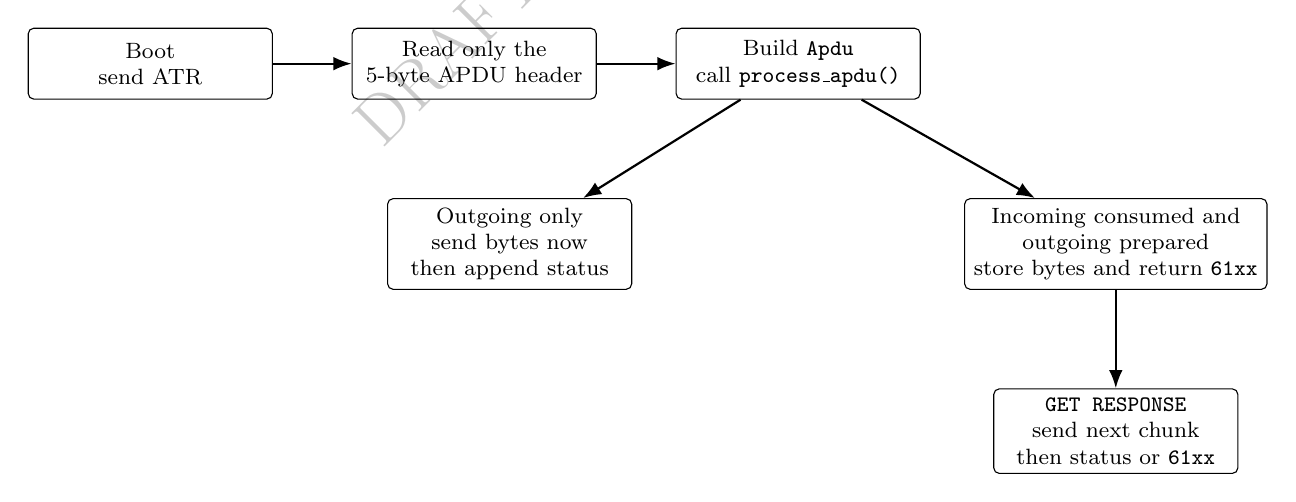
\begin{tikzpicture}[
    stage/.style={
      draw,
      rounded corners=2pt,
      minimum width=3.1cm,
      minimum height=0.9cm,
      align=center,
      font=\footnotesize
    },
    arrow/.style={->, thick, >=Latex}
  ]
    \node[stage] (atr) {Boot\\send ATR};
    \node[stage, right=1.0cm of atr] (hdr) {Read only the\\5-byte APDU header};
    \node[stage, right=1.0cm of hdr] (proc) {Build \texttt{Apdu}\\call \texttt{process\_apdu()}};
    \node[stage, below left=1.25cm and 0.55cm of proc] (direct) {Outgoing only\\send bytes now\\then append status};
    \node[stage, below right=1.25cm and 0.55cm of proc] (deferred) {Incoming consumed and\\outgoing prepared\\store bytes and return \texttt{61xx}};
    \node[stage, below=1.25cm of deferred] (getresp) {\texttt{GET RESPONSE}\\send next chunk\\then status or \texttt{61xx}};

    \draw[arrow] (atr) -- (hdr);
    \draw[arrow] (hdr) -- (proc);
    \draw[arrow] (proc) -- (direct);
    \draw[arrow] (proc) -- (deferred);
    \draw[arrow] (deferred) -- (getresp);
  \end{tikzpicture}
  \caption{Current \texttt{T=0} APDU exchange flow in the reference implementation.}
  \label{fig:impl-apdu-exchange}
\end{figure}

The transport-owned APDU session keeps the five header bytes in
dedicated scalar fields and exposes a separate fixed data buffer of
\texttt{256} bytes
for command or response data. This matches the current short-APDU
scope, avoids dynamic allocation on the transport path, and stays close
to the Java Card idea of a single APDU work buffer. The base
\texttt{T=0} manager retains ownership of actual byte emission
decisions, while command
handlers only observe an APDU-facing surface that can request
``incoming'', ``outgoing'', and ``outgoing length'' transitions.

\subsection{APDU Implementation Surfaces}
\label{sec:impl-apdu-surfaces}

At this stage, the implementation deliberately separates APDU handling
into six levels, each with a different responsibility.

\begin{itemize}
\item \textbf{Byte transport.} The \texttt{TransportLayer} trait owns
  only byte emission and byte reception. In the current reference
  implementation it is instantiated either as a serial backend or as a
  scripted in-kernel simulator.
\item \textbf{Base \texttt{T=0} manager.} The
  \texttt{T0ApduManager<T>} object is built on top of a
  \texttt{TransportLayer}. It owns the current \texttt{T=0} exchange
  state: the five header bytes, the transport buffer, the deferred
  response buffer, and the logic for \texttt{61xx},
  \texttt{GET RESPONSE}, and final \texttt{SW1/SW2} emission.
\item \textbf{Composable APDU layers.} The \texttt{ApduLayer} trait is
  the protocol-layer boundary above \texttt{T=0}. It exposes command
  reception and completion through \texttt{ApduCommand} and
  \texttt{ApduCompletion}, so higher protocol layers do not need to
  know the concrete transport-owned APDU representation.
\item \textbf{Kernel APDU view.} The kernel exposes a narrower
  \texttt{Apdu} view over that transport state. This is the object used
  by kernel-side command handlers such as the current
  \texttt{kernel\_main\_app}.
\item \textbf{Shared Rustlet ABI buffer.} When a selected Rustlet is
  called, the kernel stages the current command into a fixed-layout
  \texttt{RustletCtx}. This ABI object contains the header fields, the
  current status word, direction metadata, and one fixed payload area.
\item \textbf{Common APDU trait.} Both the kernel-side \texttt{Apdu}
  view and the Rustlet-side \texttt{RustletCtx} implement the common
  \texttt{SEApdu} trait. This is the normalization point of the current
  implementation: kernel handlers, Rustlet handlers, and the
  kernel-to-Rustlet bridge expose the same conceptual APDU operations.
\end{itemize}

This layering is important. \texttt{SEApdu} is not the transport object
itself. \texttt{ApduLayer} is not the card-side processing interface
either. \texttt{SEApdu} is the card-side processing interface of ``the
APDU currently being handled''. In other words:
\begin{itemize}
\item \texttt{TransportLayer} owns bytes on the wire;
\item \texttt{T0ApduManager} owns the \texttt{T=0} state machine;
\item \texttt{ApduLayer} owns protocol-layer composition above
  \texttt{T=0};
\item \texttt{SEApdu} owns the command-processing view seen by command
  logic.
\end{itemize}

The present implementation therefore keeps transport semantics in the
kernel while still giving both kernel-side code and Rustlets a common
APDU vocabulary. This is the main reason why the current
\texttt{kernel\_main\_app} and selected-Rustlet dispatch path can be
written against the same card-side APDU concepts while the byte-level
\texttt{T=0} policy remains centralized below them.

The current runtime stack instantiated by the kernel is therefore:
\begin{center}
\texttt{TransportLayer $\rightarrow$ T0ApduManager $\rightarrow$ ApduLayer wrappers $\rightarrow$ dispatcher $\rightarrow$ SEApdu}
\end{center}

At the time of writing, the wrapper chain contains a pass-through layer,
the generic secure-channel layer, and a small tracing layer used for scripted
debug runs. The secure-channel layer owns the APDU boundary for SCP03 and
SCP11 establishment. It also owns protected-command unwrapping and
protected-response wrapping.

\subsection{Implementation Impact of Timing Constraints}

Section~\ref{sec:apdu-t0-timing} explained the transport-level timing
constraint in general terms. In the present implementation, this leads
to a very concrete coding rule: the main loop must keep the
transmit/receive transition points adjacent in the control flow.

In particular, the implementation intentionally treats the following
boundaries as hot:

\begin{itemize}
\item after the ATR has been emitted, the code must branch immediately
  to the command-reception loop;
\item after the five-byte header has been read, the code must hand
  control immediately to the APDU handler so that an incoming payload
  can be received without unrelated work being interposed;
\item after \texttt{SW1/SW2} has been emitted, the code must fall back
  immediately to the next command reception;
\item after a deferred-response \texttt{61xx} status, the code must be
  ready to receive \texttt{GET RESPONSE} without adding unrelated work
  on the path.
\end{itemize}

This is why the current \texttt{gp\_kernel} main loop is deliberately
minimal and places comments directly at these transition points in the
source code. The goal is not to claim formal timing conformance from a
single software structure, but to make the hot path explicit and to
avoid accidental regressions caused by debug output, bookkeeping, or
other apparently harmless additions at the wrong place.

The current APDU-facing helpers implement the following contract:

\begin{itemize}
\item \texttt{set\_incoming\_and\_Receive()} reads exactly
  \texttt{Lc} bytes from the serial link into the APDU data buffer and
  marks the APDU as having consumed incoming data;
\item \texttt{set\_outgoing()} marks the APDU as an outgoing exchange
  and returns the current \texttt{Le} interpretation;
\item \texttt{set\_outgoing\_length(length)} declares how many outgoing
  bytes are prepared and constrains the writable outgoing slice to that
  length.
\end{itemize}

These names are the intended public command-processing vocabulary. The
kernel uses idiomatic Rust internally where useful, while the conceptual
APDU interface is intentionally aligned with Java Card.
The Rustlet runtime also provides \texttt{send\_bytes()} and
\texttt{send\_bytes\_long()} as convenience operations layered on top of the
same APDU buffer and outgoing-length declaration.

This last point is the main \texttt{T=0} design constraint of the
current implementation. A command is allowed to read incoming data and
to prepare outgoing data in the same logical transaction, but the
response bytes are never emitted directly by the handler itself.
Instead, the base \texttt{T=0} manager checks two facts after command
processing returns:

\begin{itemize}
\item whether the APDU object has prepared outgoing data;
\item whether the same APDU has already consumed incoming data.
\end{itemize}

If outgoing data exists and no incoming payload was consumed, the base
\texttt{T=0} manager sends the prepared bytes immediately and then appends
\texttt{SW1/SW2}. If outgoing data exists and incoming data was
consumed, the manager copies the response bytes into its own pending
response buffer, returns a status word of the form \texttt{61xx}, and
waits for a subsequent \texttt{GET RESPONSE} command. The deferred
buffer is therefore owned by the \texttt{T=0} manager rather than by the
\texttt{Apdu} object itself.

The current \texttt{GET RESPONSE} recognition rule is intentionally
small:

\begin{itemize}
\item \texttt{INS = C0};
\item \texttt{P1 = 00};
\item \texttt{P2 = 00}.
\end{itemize}

When such a command is received, the \texttt{T=0} manager handles it
itself rather than forwarding it to command logic. The
pending response buffer then emits up to the requested number of bytes
and either:

\begin{itemize}
\item returns the final completion status when the buffered response has
  been fully drained;
\item or returns another \texttt{61xx} if additional response bytes
  remain to be fetched.
\end{itemize}

In the current short-buffer implementation, a \texttt{GET RESPONSE}
command with \texttt{Le = 00} is interpreted as a request for
\texttt{256} bytes, matching the conventional \texttt{T=0} short-length
encoding.

The expected status values at this stage are therefore:

\begin{itemize}
\item \texttt{9000}: normal success, used when a command completes
  without deferred response data, or after the last successful
  \texttt{GET RESPONSE} chunk has been sent;
\item \texttt{61xx}: response bytes are pending and must be retrieved by
  \texttt{GET RESPONSE}; \texttt{SW2} carries the currently remaining
  byte count, with \texttt{00} representing \texttt{256} remaining
  bytes in the current fixed-buffer implementation;
\item \texttt{6985}: conditions not satisfied; used when a
  \texttt{GET RESPONSE} is received without any pending response, or
  when another command is received while deferred response bytes are
  still waiting to be fetched;
\item \texttt{6D00}: instruction not supported; currently the default
  result returned by \texttt{process\_apdu()} for all unimplemented
  commands.
\end{itemize}

This yields three distinct completion paths:

\begin{verbatim}
// Direct outgoing path
let le = apdu.set_outgoing();
apdu.set_outgoing_length(response_len);
let buffer = apdu.buffer_mut();
buffer[..response_len].copy_from_slice(response_data);
// T0ApduManager then appends SW1/SW2
\end{verbatim}

\begin{verbatim}
// Deferred T=0 path
apdu.set_incoming_and_Receive();
let le = apdu.set_outgoing();
apdu.set_outgoing_length(response_len);
let buffer = apdu.buffer_mut();
buffer[..response_len].copy_from_slice(response_data);
// T0ApduManager stores the response, returns 61xx,
// then waits for GET RESPONSE
\end{verbatim}

\begin{verbatim}
// Wrong Le for a pure outgoing command
let le = apdu.set_outgoing();
apdu.set_outgoing_length(actual_len);
// T0ApduManager compares requested Le and actual_len
// and may return 6Cxx instead of the payload
\end{verbatim}

The detailed correspondence between these APDU-facing operations and the
underlying \texttt{T=0} byte stream is summarized in
Appendix~\ref{app:apdu-over-t0}.

\section{Application Lifecycle Management}
\label{sec:impl-lifecycle}

Chapter~4 defines the lifecycle contract retained by Oxide SE. The reference
kernel implements that contract at the object-registry boundary: every managed
object carries a kind-specific lifecycle state, and APDU handlers consult that
state before allowing the operation family that would make the object effective.

The implemented state families are deliberately small:
\begin{itemize}
\item packages are \texttt{Loaded} or \texttt{Locked}; only
      \texttt{Loaded} packages may be used by \texttt{INSTALL [for install]};
\item ordinary instances are \texttt{Selectable} or \texttt{Locked}; only
      \texttt{Selectable} instances may be selected;
\item Security Domain instances are \texttt{Selectable} or \texttt{Locked};
      only \texttt{Selectable} Security Domains may be selected or used to
      establish a secure channel;
\item key objects are \texttt{Active} or \texttt{Locked}; only
      \texttt{Active} keys may be consumed by secure-channel establishment.
\end{itemize}

Deletion is represented by absence from the registry. Failed or interrupted
deployment is represented by the absence of a newly committed registry entry.
This avoids publishing half-created packages or instances as stable managed
objects.

\subsection{LOAD Command Handling}
\label{sec:impl-load}

The normative \texttt{INSTALL [for load]} and \texttt{LOAD} APDU shapes are
described in Section~\ref{sec:gp-install-command}. The kernel implements them
as one volatile dynamic-load transaction. \texttt{INSTALL [for load]} records
the selected authority Security Domain, the target Security Domain, the package
AID, the announced size, and the expected hash. It does not publish a package
object in the registry.

Each following \texttt{LOAD} command must target the same authority and arrive
with the next expected block number in \texttt{P2}. The final block is marked
by \texttt{P1}. The kernel rejects out-of-order blocks, size overflow beyond
the announced length, authority mismatch, and final hash mismatch. Any APDU
that is not part of the active load sequence cancels the volatile context.

Only the final valid \texttt{LOAD} block commits the package as a registry
object in state \texttt{Loaded}. Because the registry is mutated only at this
final point, a reset or power loss during the load sequence falls back to the
previous committed registry view.

\subsection{INSTALL Command Handling}
\label{sec:impl-install}

The normative command family is described in
Section~\ref{sec:gp-install-command}. This subsection only describes the
reference-kernel path for the implemented \texttt{INSTALL [for install]} case:
binding an already known package to a new selectable instance, optionally
creating a Security-Domain instance, and initializing the Rustlet state that
will later be serialized in the registry.

The kernel accepts the \texttt{INSTALL [for install]} shape identified by
\texttt{P1 = 0C} and \texttt{P2 = 00}. The command data is parsed as the
GlobalPlatform length-value sequence:
\begin{itemize}
\item package AID;
\item applet or module AID;
\item application instance AID;
\item privilege bytes;
\item install parameters.
\end{itemize}

Empty package, applet, or instance AIDs are rejected, and the privilege field
is bounded to the three-byte administrative form used by the Security-Domain
model described in Chapter~4. Malformed LV data is rejected before any registry
mutation or Rustlet call is attempted.

The management authority is resolved before installation. A clear
\texttt{INSTALL} command is interpreted under the root Security Domain
authority, and is accepted only if that backend explicitly permits out-of-band
management. A protected \texttt{INSTALL} command is interpreted under the
Security Domain bound to the authenticated secure-channel session, after the
unwrap path described in Section~\ref{sec:impl-scp-ext}. In both cases, the
kernel asks the authority to approve the operation family before it mutates the
registry. These checks cover Security-Domain and registry-plane access,
management of the target package/applet/instance triple, making the target
selectable, and the profile-specific installation policy hook.

If the requested object is a kernel-native Security Domain instance, the
kernel does not enter a Rustlet image. It creates the Security-Domain registry
object directly, attaches it to the authority Security Domain through
\texttt{parent\_sd\_aid}, and stores the encoded administrative state derived
from the install privilege bytes. This is the path used for
\texttt{NullSecurityDomain} and \texttt{KernelSecurityDomain} instances.

Otherwise, installation targets a Rustlet package already present in the
registry. The kernel resolves the package/applet pair in the active
Security-Domain view, activates the selected Rustlet image as the new instance,
and fills the shared Rustlet context with a compact LV payload containing the
same package AID, applet AID, instance AID, privilege bytes, and install
parameters. The Rustlet runtime receives that payload through its
\texttt{install()} handler, as described in
Section~\ref{sec:impl-rustlet-runtime}. The implementation deliberately avoids
building a second transport APDU for this call; the installation payload is
encoded directly into the shared Rustlet ABI buffer.

After a successful Rustlet \texttt{install()} return, the kernel saves the
instance state into the global object registry under the authority Security
Domain. Ordinary Rustlet instances are stored as instance objects with
serialized state. Rustlet-backed Security Domains additionally expose the
Security-Domain dispatch vtable described in Section~\ref{sec:impl-sd-profiles}
and keep their kernel-enforced privilege floor in the Security-Domain registry
object. A failed install call, a failed authorization check, or a failed state
save leaves no successfully selectable instance behind.

At this layer, lifecycle handling is intentionally direct: successful package
loading creates a \texttt{Loaded} package, successful installation creates a
\texttt{Selectable} instance or Security Domain, and authorized
\texttt{SET STATUS} commands lock or unlock those objects. \texttt{SELECT}
itself only changes the current execution context.

\subsection{DELETE Command Handling}
\label{sec:impl-delete}
% --- DELETE command handling ---
% This subsection describes how the DELETE command is implemented.
% It should cover:
% - validation of AIDs to delete
% - dependency checking (applications vs packages)
% - prevention of deletion of active or selected applications
% - registry update and consistency enforcement
% - memory and resource reclamation
% - rollback or failure handling

\tbc

\subsection{Lifecycle State Machine}
\label{sec:impl-lifecycle-sm}

The kernel stores lifecycle state inside the polymorphic object-registry
payload, not in a parallel table. The state bits are persisted with registry
entries, so a locked package, instance, Security Domain, or key remains locked
after reboot when persistent storage is available.

The current transition causes are:
\begin{itemize}
\item successful dynamic load commits a package as \texttt{Loaded};
\item successful \texttt{INSTALL [for install]} commits a
      \texttt{Selectable} ordinary instance or Security Domain;
\item successful \texttt{PUT KEY} commits a key object as \texttt{Active};
\item \texttt{DELETE} removes the addressed registry object after authority
      and dependency checks;
\item \texttt{SET STATUS} toggles packages, ordinary instances, and Security
      Domains between their usable state and \texttt{Locked}.
\end{itemize}

The guards are checked where the protected operation starts. Package state is
checked during package lookup for \texttt{INSTALL [for install]}; instance and
Security Domain selectability is checked during \texttt{SELECT};
Security-Domain selectability is checked before secure-channel establishment;
key state is checked while resolving SCP03 key material.

\texttt{SET STATUS} is handled as a management command. The APDU layer resolves
the authority exactly as for other management operations: a protected command is
interpreted under the Security Domain bound to the secure channel, while a
clear command is interpreted under the root Security Domain. The target object
must be reachable from that authority. Clear \texttt{SET STATUS} is accepted
only when the authority explicitly permits it; this is true for
\texttt{NullSecurityDomain} development images and false for kernel-native and
Rustlet-backed production Security Domains. Rustlet-backed Security Domains
receive a \texttt{set\_status()} authorization hook through the same dispatch
bridge used by \texttt{INSTALL}, \texttt{DELETE}, \texttt{PUT KEY}, and
\texttt{STORE DATA}.

\subsection{GET STATUS Implementation}
% --- GET STATUS implementation ---
\label{sec:impl-get-status}

The implementation parses only the modern GlobalPlatform TLV form described
in Section~\ref{sec:gp-get-data-discovery}. The mandatory \texttt{4F} search
criterion is canonicalized into a bounded AID value; the optional \texttt{5C}
tag list is structurally validated. Unsupported object families or response
formats fail before registry traversal.

Traversal follows stable registry slot order. For every live slot, the kernel
checks the requested family, AID prefix, lifecycle state and visibility from
the active Security Domain authority. Package, ordinary-instance and
Security-Domain objects are encoded directly as \texttt{E3} records in the
APDU response buffer. Key and generic-data objects are never candidates.

If the next matching record does not fit, the response ends with
\texttt{63 10}. The continuation cursor contains only:

\begin{itemize}
\item the authority AID;
\item the canonical query;
\item the index of the next registry slot.
\end{itemize}

The next command must repeat that query with \texttt{P2 = 03}. A different
query, a different authority, or any intervening non-\texttt{GET STATUS}
command invalidates the cursor. This prevents continuation under a changed
security context and avoids retaining a copy of any registry object.

The encoder is allocation-free. It first computes the exact short BER-TLV
record length, then writes directly into the remaining APDU payload. Thus
pagination is determined by the transport capacity rather than by an
intermediate response array.

% --- Cryptographic primitive layer ---
% This section describes:
% - minimal crypto API exposed by core
% - opaque AES key representation
% - in-place buffer-oriented operations
% - target-specific hardware hooks
% - software fallback strategy
\section{Cryptographic Primitive Backend}
\label{sec:impl-crypto-backend}

Before discussing key storage and SCP03 session handling, the reference
implementation needs a small cryptographic primitive layer. This layer is not
meant to expose a large application-facing crypto API. Its role is narrower:
to provide the primitive operations required by SCP03 and by platform key
management, while keeping the implementation compatible with constrained
embedded targets and with future hardware-assisted ports.

The current design therefore adopts three explicit choices.

First, the public API is buffer-oriented and keeps allocation out of the
cryptographic path. Command processing and secure-channel wrapping already
operate on preallocated APDU buffers, so the crypto layer should follow the
same model.

Second, AES keys are represented through an opaque \texttt{AesKey} type. The
caller can construct such a key from raw bytes, but does not manipulate the
internal representation directly. This leaves room for later target-specific
formats, key-slot indirections, or hardware key handles without changing the
higher-level SCP03 code.

Third, the backend selection is intentionally asymmetric:
\begin{itemize}
\item a target-specific hardware implementation should be preferred whenever a
  serious port exposes constant-time AES support or a dedicated cryptographic
  peripheral;
\item a software implementation must remain available as a fallback, both for
  boards without accelerators and for bring-up under emulation.
\end{itemize}

For the current project stage, the minimal API retained in \texttt{core} is:
\begin{itemize}
\item \texttt{fill\_random(buf)} for entropy or challenge generation;
\item \texttt{aes\_cbc\_encrypt\_in\_place(key, iv, buf)} for block-aligned
  in-place encryption;
\item \texttt{aes\_cbc\_decrypt\_in\_place(key, iv, buf)} for block-aligned
  in-place decryption;
\item \texttt{aes\_cmac(key, input, out)} for CMAC computation;
\item \texttt{scp03\_kdf(...)} for the SCP03 session-derivation path, with the
  derivation constant, context, and output buffer provided explicitly by the
  caller.
\end{itemize}

The in-place form of the CBC helpers is deliberate. In a constrained runtime,
it is highly desirable that input and output may be the same buffer. This keeps
the interface close to the APDU transport model and avoids needless scratch
buffers when wrapping or unwrapping secure messages.

The current reference implementation also assumes that the present QEMU targets
do not expose a cryptographic accelerator usable by the project at this stage.
As a consequence, the portable fallback path is the relevant one for current
development and test environments.

The runtime distinguishes explicitly between the board itself and the
execution environment. The build flow injects:
\begin{itemize}
\item \texttt{OXIDE\_SE\_BOARD} to select the supported target board;
\item \texttt{OXIDE\_SE\_EXECUTION\_ENV} to distinguish a hardware-oriented build
  from a QEMU-oriented one.
\end{itemize}

This second dimension matters because some services depend on the actual
execution context rather than on the nominal board identity alone. The same
\texttt{STM32F405} board support, for instance, should use the on-chip RNG on
real hardware but must not assume that the corresponding QEMU model exposes
that peripheral.

Among available open implementations, the RustCrypto AES crate is a credible
reference for that fallback path \cite{rustcrypto-aes}. Its public
documentation states that its implementations are designed to execute in
constant time, either through hardware intrinsics when available or through a
portable bitsliced backend otherwise. This does not eliminate the need for
review, integration discipline, and platform-specific testing, but it provides
a reasonable software baseline for the present project stage.

The random-generation path is treated more conservatively than the AES path.
For entropy generation, the project does not currently accept a purely
deterministic software fallback with no external entropy source. The NIST
\texttt{SP 800-90} family explicitly separates the role of entropy sources from
that of deterministic generators: a DRBG construction is expected to be fed by
an entropy source rather than to replace it \cite{nist80090b,nist80090c}. For
that reason, the default behavior of \texttt{fill\_random()} remains an
explicit error whenever no credible entropy source has been wired for the
current target.

For the supported STM32 hardware targets, the intended production path is to
use the on-chip RNG peripheral directly. Both STM32F405 and STM32L475 expose a
dedicated RNG block with a control register, a status register, and a data
register. The usage pattern is straightforward:
\begin{itemize}
\item initialize the peripheral once during the crypto-backend startup path;
\item enable the appropriate clock source for the target;
\item enable the RNG peripheral;
\item wait until the data-ready flag indicates that a fresh 32-bit word is
  available;
\item read the data register;
\item reject or reinitialize on hardware entropy error flags.
\end{itemize}

In practice, the generation latency documented by ST is on the order of a few
dozen peripheral clock cycles per 32-bit word, which is small enough that the
reference design does not currently require any software ``diversification'' or
PRNG expansion layer on top of the hardware output. A simple implementation may
therefore block until the status bit becomes ready and then return the newly
read word. A more optimized implementation may keep one prefetched word in
flight in order to overlap the wait for the next sample, but this remains an
optimization of the same basic hardware-driven design.

The QEMU situation is different. The currently used STM32 board models do not
provide the corresponding RNG device \cite{qemu-stm32}. The present
implementation therefore does not try to emulate a fake TRNG in software.
Instead, QEMU-oriented builds use a distinct development path selected through
\texttt{OXIDE\_SE\_EXECUTION\_ENV=qemu}: \texttt{fill\_random()} is serviced through
semihosting file access to the host \texttt{/dev/urandom}. This keeps the
development path explicit and separate from the production hardware path, while
avoiding the introduction of an ad hoc software-only generator inside the
guest.

This QEMU-only entropy bridge should not be confused with a production entropy
source. It is a bring-up facility that depends on host cooperation and on the
availability of semihosting. The default policy for unsupported environments
still remains an explicit error rather than a silently invented random stream.

More generally, the existence of a QEMU execution mode must not be read as a
security claim about the emulated target. The current QEMU path is a prototype
and validation aid. It is intentionally useful for debugging, but precisely for
that reason it relies on mechanisms that are inappropriate as part of a secure
deployment story. In particular, semihosting gives the guest controlled access
to host services and is explicitly documented by QEMU as a development-oriented
facility rather than as an isolation-preserving boundary
\cite{qemu-security,qemu-semihosting}. The QEMU runtime is therefore a
convenience environment for bring-up and test, not a substitute for the
security properties expected from the real hardware platform.

This mirrors another already known limitation of the current QEMU bring-up,
namely the lack of usable flash support in the emulated environment.

From an architectural point of view, this section should be read as a lower
layer than the next two ones:
\begin{itemize}
\item the key-management layer decides how static SCP03 keys are stored,
  versioned and updated;
\item the secure-channel layer consumes those keys and invokes the primitive
  backend to derive \texttt{S-ENC}, \texttt{S-MAC}, and \texttt{S-RMAC}, then
  to compute \texttt{C-MAC}, \texttt{R-MAC}, and protected payloads.
\end{itemize}

In a mature hardware port, the same high-level API should therefore dispatch to
target hooks that exploit the actual silicon capabilities, while preserving the
software fallback for development, unsupported boards, and test environments.

% --- Key management and secure storage ---
% This section describes:
% - internal representation of keys (key sets, versions, identifiers)
% - secure storage mechanisms
% - key update policies (PUT KEY)
% - diversification and derivation
% - protection against leakage
\section{Key Management and Secure Storage}
\label{sec:impl-key-management}

The current implementation uses the global registry for resident packages,
application instances, Security Domain instances, and cryptographic key
objects attached to those Security Domains. At the time of writing, the first
implemented key-object family is SCP03 static communication keys.

This means that the registry stores four broad classes of objects:
\begin{itemize}
\item packages carrying executable binary code;
\item ordinary application instances carrying serialized state;
\item Security Domain instances and their administrative state;
\item typed key objects attached to a Security Domain instance, currently
      SCP03 static keys.
\end{itemize}

For these ancillary key objects, the ownership rule is the same as for other
managed entities: each object is attached to one owning Security Domain
instance through \texttt{parent\_sd\_aid}. Key metadata is held in dedicated
registry fields, while the payload contains the raw key bytes consumed by the
secure-channel implementation.

In the current subset, one SCP03 key object records:
\begin{itemize}
\item a key-version number;
\item a key identifier / keyset identifier;
\item a usage selector (\texttt{ENC} or \texttt{MAC});
\item a key state, currently \texttt{Active} or \texttt{Locked};
\item one AES-128 static key value.
\end{itemize}

The current \texttt{PUT KEY} implementation therefore behaves as follows:
\begin{itemize}
\item the active Security Domain authorizes the command through the normal
      management boundary;
\item the kernel decodes the GlobalPlatform reference controls: the low seven
      bits of \texttt{P1} carry the key version, the high bit of \texttt{P1}
      carries the last-command flag, the low seven bits of \texttt{P2} carry
      the first key identifier, and the high bit of \texttt{P2} indicates
      whether the command contains several keys;
\item the kernel parses the payload entries
      \texttt{(usage, key\_len, key\_bytes)};
\item each accepted entry is stored as one serialized registry object attached
      to the active Security Domain instance;
\item when several payload entries are present, their effective key
      identifiers increment from the first identifier decoded from
      \texttt{P2};
\item storing an already existing
      \texttt{(parent\_sd\_aid, key\_version, key\_id, usage)} tuple rotates
      the key material by replacing the registry object atomically;
\item later \texttt{INITIALIZE UPDATE} resolves the requested
      \texttt{(key\_version, key\_id)} pair by reading back the corresponding
      \texttt{ENC} and \texttt{MAC} objects from the registry and rebuilding
      the \texttt{StaticKeys} structure consumed by the pure SCP03 engine.
\end{itemize}

\texttt{Locked} key objects remain present in the registry for policy and
audit-oriented evolution, but they are ignored by SCP03 session derivation.
Deletion helpers operate on the same owner-qualified tuple, so deleting one
usage or keyset member cannot remove a sibling Security Domain's key.

This storage rule is shared by both secure backends currently implemented in
Oxide SE:
\begin{itemize}
\item kernel-native Security Domains resolve those registry-backed key objects
      directly inside the kernel;
\item Rustlet-backed Security Domains reached through
      \texttt{RustletSecurityDomainProxy} load the same key objects through
      runtime syscalls and derive their SCP03 sessions in user-land.
\end{itemize}

Two consequences are important:
\begin{itemize}
\item SCP03 static key material is stored as Security Domain-owned registry
      objects;
\item identical \texttt{(key\_version, key\_id, usage)} tuples may exist in
      several Security Domain subtrees, because the corresponding key objects
      are qualified by \texttt{parent\_sd\_aid}.
\end{itemize}

This organization keeps an important implementation invariant intact:
cryptographic material is not hidden in ad hoc side tables unrelated to the
registry model. The registry remains the common persistence and authority
surface for applications, Security Domains, and the ancillary objects they
own.

For the root kernel-native Security Domain, the bootstrap path already inserts
the static SCP03 key objects explicitly declared under \texttt{root.keys} in
the build manifest. Supplementary Security Domains use the equivalent
\texttt{security\_domains.keys} declaration. The very first
\texttt{INITIALIZE UPDATE} therefore consumes registry-backed key material
rather than a side-loaded session secret, and a manifest without keys receives
no implicit development fallback. The same registry model is also used by the
Rustlet-backed Security Domain path; its difference is not the storage model,
but where session derivation is executed.

The remaining work in this area is not the existence of registry-backed keys
themselves, but the richer GlobalPlatform policy surface around them:
additional usages, rotation semantics, diversification, production
provisioning, and the final policy for first-key provisioning of supplementary
Security Domain instances.


\section{Secure Channel Implementation}
\label{sec:impl-scp}

Oxide SE implements secure channels as a kernel-mediated protocol stack whose
active Security Domain backend may be kernel-native or Rustlet-backed. The
current implementation is intentionally split into four layers:

\begin{itemize}
\item protocol-specific pure cryptographic engines
      (\texttt{core::scp03}, \texttt{core::scp11}) with no dependency on APDU
      routing, registry state, or Security Domain policy;
\item \texttt{core::gp\_sm}, which centralizes the bounded payload budgets
      imposed by Amendment~D command and response MAC trailers;
\item the active Security Domain backend, which owns policy decisions, static
      keys, session lifecycle, and secure-messaging state;
\item \texttt{SecureChannelLayer}, which owns the APDU boundary: command
      interception, command unwrapping, response wrapping, and management
      command authorization for the supported SCP profiles.
\end{itemize}

This split is the main implementation invariant. Cryptographic transforms are
not scattered through the APDU dispatcher, and the cryptographic core does not
know how an AID is installed, selected, or stored in the registry.

The active backend may take three forms:
\begin{itemize}
\item a pseudo-Security-Domain path (\texttt{NullSecurityDomain}) for bring-up
      and test scenarios;
\item a kernel-native Security Domain path (\texttt{KernelSecurityDomain});
\item a Rustlet-backed Security Domain path reached through
      \texttt{RustletSecurityDomainProxy}.
\end{itemize}

In every case, the secure-channel session is associated with one Security
Domain instance and one logical channel. The current implementation still
provides only one effective channel, but the authority boundary is already
framed in those terms rather than as a single process-global SCP state.

\subsection{Security Domain Profiles}
\label{sec:impl-sd-profiles}
\label{sec:impl-scp-profiles}

The default management selector is configured by the predeployment manifest.
The root Security Domain backend is declared under \texttt{[root.package]},
while the secure-channel protocols compiled into the image are declared under
\texttt{[secure\_channel]}. Three Security Domain backends are currently
accepted:

\begin{itemize}
\item \texttt{NullSecurityDomain}, a no-security/debug authority that
      authorizes management operations and does not establish SCP sessions;
\item \texttt{KernelSecurityDomain}, a kernel-native Security Domain whose
      supported SCP profiles are selected by \texttt{protocols},
      \texttt{scp03\_profile}, and \texttt{scp11\_profiles};
\item \texttt{RustletSecurityDomainProxy}, a kernel-side proxy that delegates
      Security-Domain policy and SCP state to one selected Rustlet Security
      Domain instance while preserving kernel-owned base privileges.
\end{itemize}

The S8 and S16 variants are explicit secure-channel profiles rather than
distinct administrative authorities. A manifest that enables SCP03 therefore
declares \texttt{scp03\_profile = "S8"} or
\texttt{scp03\_profile = "S16"}. A manifest that enables only SCP11 omits the
SCP03 profile entirely and declares its supported SCP11 variants through
\texttt{scp11\_profiles}, for example \texttt{["A", "C"]}. The internal engine
is shared, and one \texttt{KernelSecurityDomain} implementation exposes the
same \texttt{SecurityDomainManagement} and
\texttt{SecurityDomainSecureChannel} traits regardless of the selected SCP
combination.

The proxy variant keeps those same kernel-side traits and APDU boundaries, but
forwards the dedicated Security-Domain operations through \texttt{sddispatch}
to the currently selected Rustlet Security Domain instance. The kernel still
owns APDU parsing, registry mutation, non-escalation checks, and active-context
tracking; the Rustlet Security Domain refines policy and performs its own SCP
cryptography through the runtime APIs.

\subsection{Selected Secure-Channel Security Levels}
\label{sec:impl-scp-selected-levels}

The reference implementation deliberately selects a strict subset of the
normative security-level matrices described in Chapter~3. This is a build and
interoperability profile, not a redefinition of the GlobalPlatform values.

For SCP03, \texttt{EXTERNAL AUTHENTICATE} accepts only
\texttt{P1 = 00}, \texttt{01}, or \texttt{03}: authenticated session without
secure messaging, C-MAC, or C-MAC with C-ENC. The response-protection levels
\texttt{11}, \texttt{13}, and \texttt{33} are rejected explicitly with
\texttt{6985}. Consequently, responses in the selected SCP03 profile remain
plain; the optional \texttt{BEGIN R-MAC SESSION} and
\texttt{END R-MAC SESSION} commands are profiled out and return
\texttt{6D00}.

For SCP11a, SCP11b, and SCP11c, the CRT accepts only key-usage qualifier
\texttt{95 01 3C}, selecting C-MAC, C-ENC, R-MAC, and R-ENC. The GP-defined
\texttt{34} alternative is rejected for all three variants; the SCP11c-only
\texttt{1C} and \texttt{74} alternatives are rejected as well. SCP11 does not
define the explicit R-MAC session companion commands: response protection is
part of the security level established by the CRT.

The authenticated-peer class is also part of the selected profile and is
applied before any Security Domain hook:
\begin{itemize}
\item SCP03 and owner-authenticated SCP11a may carry the implemented
      management command families;
\item SCP11b authenticates the card, not the OCE, and is consequently limited
      to read-only \texttt{GET DATA} in this implementation profile;
\item owner-authenticated SCP11c permits the implemented management families
      except \texttt{PUT KEY}, \texttt{SET STATUS}, and deletion of key
      objects, as required by the SCP11c restrictions;
\item SCP11c \texttt{ANY\_AUTH} permits \texttt{GET DATA} only. Mutating
      operations requiring the \texttt{BF20} authorization object are
      explicitly profiled out.
\end{itemize}
This matrix is a non-overridable kernel gate. The selected Security Domain's
hierarchy, privilege checks, and management hooks are then evaluated for every
accepted command and may only narrow the decision.

The implementation also supports a supplementary-protocol fallback. A
secure-channel protocol selected in the build manifest always has priority and
uses the kernel matrix above. If no selected kernel profile recognizes an
establishment command, the active Rustlet Security Domain may explicitly claim
the header and process the raw establishment data. The resulting session is
recorded as Rustlet-owned without assigning it a fictitious SCP identifier.
Protocol-specific authorization is then owned by that Security Domain, but
registry ancestry, privilege non-escalation, lifecycle checks, APDU bounds, and
management-family hooks remain enforced by the kernel. This extension point
therefore permits supplementary protocols without turning the registry into
Rustlet-controlled memory.

These choices are enforced before a session becomes authenticated. Host-based
tests exhaustively reject every other byte value, while QEMU scenarios exercise
the accepted levels and representative GP-defined but profiled-out values at
the APDU boundary.

S8 uses 8-byte host/card challenges, 8-byte authentication cryptograms, and
8-byte C-MAC/R-MAC values. S16 uses 16-byte challenges, 16-byte cryptograms,
and 16-byte MAC values. The APDU layer therefore never assumes a fixed
protected-command trailer shape. It asks the active Security Domain for the
current MAC length and session policy before separating the raw payload from
its trailing MAC.

Separately from these kernel-native profiles, Oxide SE also supports a
Rustlet-backed Security Domain path. In that case, the kernel still owns APDU
interception and routing, but the selected Security Domain instance performs
secure-channel operations through the Rustlet runtime and the generated
\texttt{sddispatch} entry.

\subsection{Pure SCP03 Engine}
\label{sec:impl-scp-core}

The pure engine in \texttt{core::scp03} defines:

\begin{itemize}
\item \texttt{Scp03Profile}, with profile-dependent lengths for S8 and S16;
\item \texttt{StaticKeys}, currently AES-128 ENC and MAC test keys;
\item \texttt{SessionKeys}, containing S-ENC, S-MAC, and S-RMAC;
\item \texttt{SessionMaterial}, produced by one
      \texttt{INITIALIZE UPDATE};
\item \texttt{SessionState}, which owns MAC chains and encryption counters for
      secure messaging;
\item \texttt{SecurityLevel}, which represents no secure messaging, SCP03
      command-only protection, and the full bidirectional protection selected
      for SCP11.
\end{itemize}

The engine derives session material from the static keys, host challenge and
card challenge using the SCP03 KDF. It then computes card and host
cryptograms, verifies the host cryptogram during authentication, validates
C-MAC on protected commands, decrypts C-ENC command data, and provides the
R-MAC/R-ENC primitives used by the common SCP11 secure-messaging path. The
selected SCP03 levels do not activate response protection; the exact selected
matrix is stated in Section~\ref{sec:impl-scp-selected-levels}.

The current implementation uses AES-CMAC and AES-CBC style encryption with
GlobalPlatform padding rules. SCP03 itself remains a symmetric protocol here:
asymmetric authentication, post-quantum key establishment, or card certificate
handling would be higher-level platform services, not requirements of the
current SCP03 core.

\subsection{APDU Layer Integration}
\label{sec:impl-scp-apdu-layer}

\texttt{SecureChannelLayer} sits above the T=0 APDU manager. It sees clear APDUs
after T=0 procedure-byte handling, but before Rustlet dispatch or management
mutation. Its responsibilities are:

\begin{itemize}
\item intercept \texttt{INITIALIZE UPDATE} and call the active Security
      Domain's secure-channel entry point;
\item intercept \texttt{EXTERNAL AUTHENTICATE}, verify the host cryptogram,
      and open the requested security level;
\item intercept \texttt{PERFORM SECURITY OPERATION} and
      \texttt{MUTUAL AUTHENTICATE} for SCP11-capable backends;
\item reject protected commands if no authenticated secure-channel session
      exists;
\item split protected command data into its raw payload and trailing
      profile-dependent C-MAC;
\item ask the Security Domain to unwrap protected command data before command
      dispatch;
\item ask the Security Domain to protect response data, append the R-MAC when
      required, and retain the actual status word before transmission.
\end{itemize}

Management commands such as \texttt{INSTALL [for install]} are still parsed and
executed by the kernel. The Security Domain authorizes them. With
\texttt{NullSecurityDomain}, this authorization is deliberately open for debug
and bootstrap scenarios. With \texttt{KernelSecurityDomain}, mutating
management commands require an
authenticated encrypted SCP03 session. The kernel-native Security Domain path
keeps a small per-instance administrative state keyed by instance
AID. At this stage that state serializes the privilege bitfield carried by
\texttt{INSTALL}, seeds the implicit root instance with the bootstrap privilege
set, and lets the kernel preserve kernel-owned administrative privilege state
without relying on a Rustlet serializer.

More generally, Security Domain instances are modeled as objects of the global
registry. Each such object may carry a \texttt{parent\_sd\_aid} and a
serialized administrative state. For a Rustlet-backed Security Domain, that
state is split between kernel-owned authority data and Rustlet-owned persistent
functional state. For \texttt{NullSecurityDomain} and kernel-native profiles,
the persistent administrative state may reduce to privilege bits. Active
secure-channel state remains volatile in every backend.

\subsection{Persistent Security-Domain State and Volatile Sessions}
\label{sec:impl-scp-state-lifetime}

The lifetime of Security-Domain configuration is distinct from the lifetime of
an authenticated secure-channel session. Registry-backed persistent state may
contain lifecycle, privileges, application policy, certificate references, or
other long-lived configuration. It shall not contain derived session keys,
expected cryptograms, receipts, command or response MAC chains, encryption
counters, or partially staged handshake buffers.

A Rustlet Security Domain expresses this boundary in its serialized Rust type.
Its secure-channel field is marked \texttt{\#[serde(skip)]} and implements
\texttt{Default}. The runtime deserializes the object when the Security Domain
FAE is loaded. The resulting Rust value remains alive in RAM while that
Security Domain is loaded, so consecutive establishment and protected APDUs
observe the same live session. The active Rustlet Security Domain remains
resident in a dedicated firmware slot while an ordinary selected Rustlet
occupies the application slot. The \texttt{unwrap}, application-dispatch, and
\texttt{wrap} calls therefore alternate between two live instances rather than
unloading and restoring the Security Domain through the registry. After each
successful \texttt{sddispatch} call, the runtime serializes only the persistent
view and publishes it through the registry. It does not reload persistent state
before every APDU.

Unloading, rebooting, or later reloading the Security Domain reconstructs the
skipped session field at its inactive default. An earlier Postcard encoding
that still carries trailing session bytes may be decoded for migration, but
those bytes are ignored and never reactivate the old channel.

Explicit \texttt{reset\_secure\_channel()} remains mandatory. A new
establishment exchange, a terminating clear command, or another session-ending
condition may occur while the Security Domain remains loaded. Reset therefore
overwrites all volatile secrets, chains, counters, cryptograms, receipts, and
staged handshake data immediately; session termination never relies on a
future deselection. Persistent mutations are still committed after successful
calls rather than being deferred until \texttt{DESELECT}, because power may be
lost before such a command occurs.

\subsection{Validation Strategy}
\label{sec:impl-scp-validation}

Validation is deliberately split into two levels. Pure cryptographic regression
tests validate deterministic SCP03 transformations for S8 and S16. QEMU
integration tests validate that those transformations are correctly connected
to APDU parsing, Security Domain policy, registry mutation, and Rustlet
execution.

The detailed vector files, their OpenSCDP/GlobalPlatformPro and Samsung
OpenSCP-Java provenance, and the exact test flows are documented in
Appendix~\ref{app:scp03-vectors}. The
important implementation point here is that the kernel does not treat S8/S16
as test-only constants: profile-dependent lengths are part of the active
Security Domain state and are consumed by the APDU secure-channel layer.

\subsection{Remaining Certification Gap}
\label{sec:impl-scp-certification-gap}

The implementation is structured for auditability, but it is not a claim of
GlobalPlatform certification. Appendix~\ref{app:scp03-vectors} documents the
current independent regression evidence. The remaining work includes:

\begin{itemize}
\item defining a secure production provisioning policy for the initial keys
      currently declared by development manifests;
\item validating ICV, chaining, counter and error behavior against official
      certification material if it becomes available to the project;
\item completing key-set lifecycle policy beyond the current registry-backed
      \texttt{PUT KEY} path, including production provisioning, rotation
      governance and diversification rules.
\end{itemize}

\section{Registry and Data Management}
\label{sec:impl-registry}
% --- Internal registry and data access ---
% This section describes:
% - internal representation of registry (AIDs, domains, privileges)
% - GET DATA / STORE DATA handling
% - persistence model
% - consistency guarantees

\subsection{GlobalPlatform Discovery Objects}
\label{sec:impl-gp-discovery}

The APDU layer resolves \texttt{GET DATA 0066} and \texttt{0067} through the
Security Domain that is authoritative for the command. Clear discovery uses
the root Security Domain; protected discovery uses the Security Domain bound
to the active secure channel.

\texttt{NullSecurityDomain} emits a complete \texttt{66/73} recognition
structure but no \texttt{64} SCP declaration, and reports
\texttt{GET DATA 0067} as absent with \texttt{6A88}.
\texttt{KernelSecurityDomain} constructs both objects from the effective build
configuration: only compiled and enabled SCP03 and SCP11 profiles are
advertised. SCP11 always advertises S16, while SCP03 reports its configured S8
or S16 option.

A Rustlet-backed Security Domain answers through its \texttt{get\_data} hook.
The runtime default constructs the same standards-compliant objects from the
SCP03 S8/S16 and SCP11a/b/c support methods. A Rustlet may override
\texttt{get\_data} for richer domain-specific data. If it advertises no
protocol, the proxy does not substitute the kernel's capabilities: discovery
describes the selected Security Domain, not the firmware in general.

All discovery objects are encoded directly in the APDU response buffer by a
bounded BER-TLV writer. No registry object, key bytes, certificate, or
intermediate response array is exposed or retained.

The firmware keeps one kernel-owned object registry. This registry is the
implementation counterpart of the GlobalPlatform object model described in
Chapter~4: it is the single catalogue for packages, application instances,
Security Domain instances, and ancillary objects such as secure-channel keys.
Security Domains do not own private registries. Instead, every registry object
is attached to an administrative Security Domain through
\texttt{parent\_sd\_aid}.

Each registry entry has a small common header:
\begin{itemize}
\item \texttt{object\_aid}, the AID by which the object is addressed;
\item \texttt{parent\_sd\_aid}, the Security Domain instance under whose
  administrative authority the object lives;
\item \texttt{kind}, which distinguishes the concrete object family.
\end{itemize}

The object kind determines the payload shape:
\begin{itemize}
\item a \textbf{package} object uses its \texttt{object\_aid} as the
  executable-load-file AID and carries the FAE binary image;
\item an \textbf{application instance} records the package AID from which it
  was instantiated and carries the serialized application state;
\item a \textbf{Security Domain instance} records the package or backend that
  implements it, the three-byte administrative privilege field, and its
  serialized administrative state;
\item a \textbf{key} object records key metadata such as version, identifier,
  usage, type and length, together with the raw key material.
\end{itemize}

The root Security Domain is not kept outside this structure. It is created by
the predeployment manifest as a real Security Domain instance with no parent,
using the backend declared under \texttt{[root.package]} and the instance AID
and installation bytes declared under \texttt{[root.instance]}. A development
image may use \texttt{NullSecurityDomain}; a protected image may use
\texttt{KernelSecurityDomain} or a Rustlet-backed Security Domain. In all
cases, the root follows the same registry shape as supplementary Security
Domains.

Registry lookup is authority-aware. A raw global lookup exists only inside the
kernel for consistency checks and bootstrap. Management operations resolve AIDs
through the active Security Domain view: the selected or secure-channel-bound
Security Domain sees itself, objects attached to it, and objects attached to
descendant Security Domains. Objects outside that subtree are treated as absent
for that administrative operation. This is the implementation form of the
visibility rule described in Section~\ref{sec:gp-object-relationships}.

Privilege delegation is checked before a Security Domain instance is created or
updated. The three-byte privilege field is kernel-owned authority data: a
Rustlet-backed Security Domain may receive the installation payload and keep
additional serialized policy state, but it cannot broaden the base
GlobalPlatform privileges that the kernel recorded for the instance. A child
Security Domain must therefore have a privilege set no broader than what its
parent is allowed to delegate.

Persistence is deliberately expressed at the registry-object level. Packages,
instances, Security Domains, and keys are the units that must eventually be
written atomically to non-volatile storage. Until the persistent backend is
implemented, the predeployment manifest rebuilds the initial registry at boot.
Once non-volatile storage is available, the same registry-object model remains
the unit of recovery: a management operation either installs, updates, or
deletes a complete registry object consistently, or it leaves the previous
registry state intact.

\section{Logical Channel and Context Management}
\label{sec:impl-channel}
% --- Logical channels and execution context ---
% This section describes:
% - channel allocation (MANAGE CHANNEL)
% - mapping channel → selected application
% - SELECT command handling
% - context switching model

The current kernel implements only the minimal selected-context model
required to bootstrap an embedded administrative application. In
GlobalPlatform terms, this is deliberately only the beginning of the
logical-channel story: there is one effective channel, one selected
context slot in the kernel, and no \texttt{MANAGE CHANNEL}
implementation yet.

At this stage, the selected context is not a high-level Rust object but
an explicit kernel-owned record containing:
\begin{itemize}
\item the application-global-pointer value returned by the loaded FAE
  image;
\item an opaque application state pointer;
\item a pointer to a C-style vtable containing the application entry
  points.
\end{itemize}

This representation is intentional. The kernel image and the loaded FAE
image are two distinct position-independent binaries, each with its own
global-pointer context. A native Rust \texttt{\&dyn Trait} would not be
an appropriate boundary here, because the call path must explicitly
switch to the application's relocation context before entering its code
and must restore the kernel context on return.

\subsection{Selected Context and Embedded Administrative Application Activation}
\label{sec:impl-selected-context}

The selected application is drawn from Rustlets packaged as independent FAE
images and declared by the predeployment manifest. Each registry package and
instance uses three GlobalPlatform-style identifiers:
\begin{itemize}
\item a \textbf{package AID}, corresponding to the executable load file;
\item an \textbf{applet AID}, corresponding to the installable module;
\item an \textbf{instance AID}, corresponding to the selectable live
  instance.
\end{itemize}

Test manifests may assign the same value to these three AIDs for compact
scenarios. They remain distinct identifiers in the registry and follow the
GlobalPlatform identification model.

The \texttt{SELECT} command remains kernel-owned. The transport loop
detects \texttt{INS = A4} before generic dispatch, requests the command
payload, interprets it as an instance AID, and compares it against the
kernel registry. If no entry matches, the kernel returns \texttt{6A82}
(file not found). If a matching entry exists, the kernel activates the
corresponding embedded FAE and records that instance as the current
selected context.

This activation follows the XiPFS FAE execution model rather than a
kernel-specific reinvention of the startup runtime. The kernel enters
the embedded image at offset \texttt{0}, thereby using the existing
XiPFS startup code unchanged. The startup path relocates the FAE image
into the application RAM arena and yields the information required to
call the application \texttt{start} entry point.

The kernel-side activation path therefore has two distinct steps:
\begin{enumerate}
\item run the FAE loader to relocate the image and obtain the
  application entry point together with the application global-pointer
  state;
\item call the application's \texttt{start(buffer)}
  function and validate the returned selected-application descriptor.
\end{enumerate}

The \texttt{buffer} currently contains the shared ABI buffer used to
carry the ABI version, APDU header fields, status word and payload. The
descriptor returned by \texttt{start()} contains:
\begin{itemize}
\item the ABI version expected by the application;
\item the current instance AID as seen from the Rustlet runtime;
\item an opaque application state pointer;
\item a vtable with two entry points:
  \texttt{install()} and \texttt{process\_apdu()}.
\end{itemize}

On the application side, the current ABI is intentionally minimalist.
An application declares one resident state type and one installation
function, then exports them through:

\begin{verbatim}
struct SecurityDomain;
declare_rustlet!(SecurityDomain, 1024usize, install);
\end{verbatim}

The \texttt{declare\_rustlet!} macro hides the internal runtime
boilerplate in \texttt{rustlet\_runtime}. The
application author therefore only needs to provide:
\begin{itemize}
\item the concrete state type later used by
  \texttt{process\_apdu()};
\item an \texttt{install()} function that constructs this state;
\item the \texttt{process\_apdu()} implementation itself.
\end{itemize}

Only after these checks does the kernel update its single selected
context slot. This is the precise meaning of selection in the current
implementation: \texttt{SELECT} does not install the application, does
not invoke the \texttt{install()} callback, and does not yet grant a
general execution mode. It merely resolves an AID to an embedded
administrative application, loads that application, and records it as
the selected execution context for subsequent command dispatch.

The later command path then uses kernel-side trampolines to enter the
selected application. These trampolines load the application's
global-pointer context before the callback and restore the kernel state
after the callback returns. This context-switching rule is the critical
mechanism that allows the kernel and the selected FAE image to coexist
without treating the application as part of the kernel's own relocation
domain.

\subsection{Rustlet Runtime, ABI and Isolation}
\label{sec:impl-rustlet-runtime}
% --- Rustlet runtime and isolation implementation ---
% This subsection should describe the concrete implementation of the
% abstract Rustlet model introduced in Chapter 7.
% It should cover:
% - the current shared ABI based on RustletCtx;
% - the declare_rustlet! macro and its generated start entry point;
% - the selected-application descriptor and vtable;
% - the current core::isolation session model;
% - MPU planning and region programming;
% - the concrete gate region layout;
% - the ARM M-profile SVC / MemManage / resume path;
% - how install, process_apdu, exit, panic and faults converge;
% - the current limits of state persistence and serialization.

The Rustlet runtime is split between two binaries. The kernel owns selection,
registry lookup, APDU transport, MPU programming and syscall dispatch. The
Rustlet image owns the application state, the Rustlet heap, the typed APDU
framework and the exported entry points expected by the kernel. The boundary
between the two is deliberately a C-style ABI rather than a native Rust trait
object, because the kernel and the Rustlet FAE image have distinct relocation
contexts.

The first entry point of a Rustlet image is the FAE entry at offset
\texttt{0}. The kernel enters this image with the shared
\texttt{RustletCtx} pointer and the application global-pointer context. The
Rustlet runtime initializes its local runtime globals, aligns the private heap
storage declared by the macro, builds a \texttt{SelectedAppDescriptor}, and
returns that descriptor through the dedicated runtime-return syscall. The
descriptor contains:
\begin{itemize}
\item an opaque runtime state pointer;
\item a selected-application vtable containing \texttt{install()} and
  \texttt{process\_apdu()} handlers;
\item an optional Security-Domain vtable for Rustlet-backed Security Domains;
\item the Rustlet heap window exported to the kernel.
\end{itemize}

The \texttt{declare\_rustlet!} macro is the developer-facing source of this
low-level structure. It generates the exported \texttt{start()} function,
allocates the static Rustlet heap storage, adapts the user installation
function into a boxed runtime instance, and wraps that instance in the runtime
persistence adapter. \texttt{declare\_app!} is only a compatibility alias.
\texttt{declare\_security\_domain!} follows the same pattern, but also exports
the \texttt{sddispatch} vtable used by
\texttt{RustletSecurityDomainProxy}.

All APDU exchange uses one shared \texttt{RustletCtx}. Before a Rustlet call,
the kernel fills the APDU header fields and stages any incoming payload in the
context payload buffer. During the call, Rustlet code normally uses the typed
\texttt{Apdu<State>} wrapper described in Chapter~7, but the ABI object remains
the same shared buffer. If the Rustlet switches to outgoing mode, the same
payload area becomes the response area. On return, the kernel publishes the
outgoing length and status word in its transport session. In firmware, the
transport payload and the Rustlet payload are two views of the same gate-region
storage, so this publication does not normally copy the payload. Normal command
completion clears the payload half. An abrupt Rustlet exit clears the complete
shared page, and every later Rustlet entry reinitializes the control half before
user code can observe it.

The shared page has two implementation-level invariants that are deliberately
stronger than the public Rustlet API. First, the APDU payload half is the only
place where Rustlet command or response payload bytes are staged. Protocol
layers must not introduce larger stack-local APDU mirrors on the hot path.
Second, the control half is also the kernel's secondary scratch buffer before a
Rustlet entry. Secure-channel code may use it while parsing, authenticating or
wrapping APDUs, but every Rustlet entry path must reset it to the ABI layout
before user code can observe the page. This is especially important when the
scratch bytes contain decrypted data, MAC material or serialized state.

The application call path is normalized around two vtable handlers. The
\texttt{install()} handler constructs the resident Rustlet instance from the
\texttt{INSTALL [for install]} parameters exposed by the kernel. The
\texttt{process\_apdu()} handler loads the current serialized state if
necessary, calls the Rustlet implementation, and saves the resident state again
before returning. A Security-Domain Rustlet uses the same selected-application
handlers for ordinary APDUs and the separate \texttt{sddispatch} handler for
kernel-initiated management, secure-channel and secure-messaging hooks.

Isolation is planned before the kernel enters the Rustlet. The current MPU plan
contains the Rustlet text window, one writable RAM block containing stack,
relocated data and heap, and the gate region. The writable Rustlet RAM block is
mapped read/write and non-executable. The Rustlet text window is mapped
executable only while the CPU is actually executing Rustlet code. When the
Rustlet traps into the kernel through a syscall, the kernel switches to a
``kernel serving Rustlet'' phase and disables execution from the active Rustlet
text regions before servicing the request. Execution permission is restored
only when control is returned to the Rustlet.

The gate region contains the shared ABI buffer and the small target-specific
entry/resume stubs required to cross the privileged/unprivileged boundary. It
is the only deliberately shared execution bridge. The rest of the Rustlet
memory map is explicit: Rustlet code cannot read or write kernel memory, cannot
execute from its writable RAM block, and cannot execute from its own text while
the kernel is servicing a syscall.

Rustlet termination paths converge through the same isolation machinery. A
normal handler return, an explicit Rustlet exit, a panic, and a recoverable MPU
fault all redirect execution back to the kernel resume point with a small
return kind and status value. For ARMv7-M targets this is primarily driven by
the MemManage path; for ARMv6-M targets without a separate MemManage exception,
the board port may translate the relevant HardFault cases into the same
recoverable application-fault path. In both cases, a fault while no Rustlet call
is active remains a kernel fault, not an application status word.

The current persistence boundary is intentionally at the serialized Rustlet
state level. The runtime adapters can load and save the resident state through
the shared context, and the kernel stores that serialized state in the registry
object for the selected instance. This is not yet a full non-volatile storage
backend: without persistent registry storage, rebooting the firmware rebuilds
the initial predeployment state. The important invariant is nevertheless
already in place: Rustlet execution sees an instance state, not a global static
singleton, and the registry object is the place where that state will become
durable once flash-backed persistence is implemented.

\section{APDU Parsing and Command Dispatch}
\label{sec:impl-apdu-dispatch}
% --- APDU parsing and command dispatch ---
% This section describes how APDU commands are decoded and dispatched
% to the appropriate handlers (LOAD, INSTALL, DELETE, etc.)

The transport mechanics of the \texttt{T=0} exchange are described in
Section~\ref{sec:impl-apdu-t0}. The APDU-facing implementation surfaces
are summarized in Section~\ref{sec:impl-apdu-surfaces}. Once the command
header has been captured, the dispatcher receives an
\texttt{ApduCommand} through the \texttt{ApduLayer} boundary, derives an
ephemeral kernel-side \texttt{Apdu} view from it, and then applies the
dispatch rules. This keeps the transport representation internal to the
base \texttt{T=0} manager and reserves the space for higher protocol
layers such as SCP03.

The dispatch layer is deliberately small and distinguishes four cases before
ordinary application-command routing:
\begin{itemize}
\item \texttt{GET RESPONSE} remains entirely transport-owned;
\item \texttt{SELECT} remains kernel-owned and updates the selected
  context as described in Section~\ref{sec:impl-selected-context};
\item GlobalPlatform management commands that mutate or query platform state
  remain kernel-owned and are authorized by the active Security Domain;
\item every other command is forwarded to the currently selected application
  through the selected-application ABI.
\end{itemize}

This organization keeps the boundary between transport, protocol-layer
composition, and command logic explicit. The base \texttt{T=0} manager
remains responsible for byte acquisition, deferred \texttt{GET RESPONSE}
handling, wrong-\texttt{Le} handling through \texttt{6Cxx}, and final
\texttt{SW1/SW2} emission. The secure-channel layer is responsible for
establishment, protected-command unwrapping, and protected-response wrapping.
The management dispatcher is responsible for the kernel-owned GlobalPlatform
operations. Only after those layers have declined a command does the ordinary
selected-application ABI receive it.

The current ABI-level exchange object is a fixed-layout
\texttt{RustletCtx} structure containing exactly two \texttt{256}-byte halves:
\begin{itemize}
\item a control/secondary buffer containing the ABI version, APDU
  header/status bytes, flags, the one-byte APDU data length and serialized
  state;
\item one fixed \texttt{256}-byte APDU payload buffer.
\end{itemize}

If the APDU requires command data reception, the kernel receives that
payload and stages it into the incoming view of this shared buffer. If
the Rustlet switches the buffer to outgoing mode, the same payload area
is then interpreted as the response buffer.

The APDU payload buffer is physically \texttt{256} bytes long, but the current
short-APDU ABI exposes at most \texttt{255} useful bytes. This is intentional:
the length field is one byte, and extended APDU support must be introduced as
an ABI evolution rather than by silently overloading the current layout. The
serialized-state slice lives in the control/secondary half and is currently
limited to \texttt{244} bytes after ABI metadata.

The kernel-to-Rustlet bridge is normalized around the
\texttt{SEApdu} trait. In practice, three APDU-facing objects implement
that common interface:
\begin{itemize}
\item the kernel-side \texttt{Apdu} wrapper;
\item the Rustlet-side \texttt{RustletCtx};
\item the kernel bridge object that couples the transport-owned APDU
  state with the shared Rustlet ABI buffer while a Rustlet call is in
  progress.
\end{itemize}

APDU command logic manipulates the current \emph{card-side APDU
session} through the common APDU interface, while transport remains
kernel-owned.

Dispatch therefore follows this kernel-owned rule:
\begin{itemize}
\item \texttt{GET RESPONSE} stays transport-owned;
\item \texttt{SELECT} stays kernel-owned and resolves an instance AID in
  the registry;
\item secure-channel establishment and protected-message framing stay in
  \texttt{SecureChannelLayer};
\item management commands such as \texttt{INSTALL}, \texttt{LOAD},
  \texttt{DELETE}, \texttt{PUT KEY}, \texttt{GET DATA}, and
  \texttt{GET STATUS}, \texttt{STORE DATA}, and \texttt{SET STATUS} stay
  kernel-owned and are authorized by the active Security Domain;
\item otherwise, the kernel calls the selected application's
  \texttt{process\_apdu()} entry point.
\end{itemize}

For \texttt{INSTALL}, the kernel parses the
GlobalPlatform \texttt{INSTALL [for install]} body as a sequence of
length-value fields:
\begin{itemize}
\item Executable Load File AID (package AID);
\item Executable Module AID (applet AID);
\item Application Instance AID;
\item privileges;
\item install parameters.
\end{itemize}

The kernel then resolves the target Rustlet from the package/applet AID
pair, updates the current instance AID, and only exposes the
\emph{install parameters} to the Rustlet-side \texttt{install()}
callback. This means that the Rustlet constructor sees the installation
payload relevant to the application itself, while the GlobalPlatform
deployment envelope remains kernel-owned.

This rule is still intentionally narrow. The goal is to validate the
boundary between the kernel and the selected administrative application
before encoding the full GlobalPlatform routing matrix. In particular,
\texttt{SELECT} itself never invokes \texttt{install()}; \texttt{INSTALL}
is an explicit command interpreted according to the GlobalPlatform body
structure before the
application callback is entered.

In the current Rustlet model, \texttt{install()} is the application-side
constructor of the selected context. The ABI has no separate definition
object.

When the selected application returns, the kernel copies outgoing bytes only
when the bridge is backed by distinct storage. The normal firmware path simply
publishes the outgoing length for the already shared payload and then resumes
the normal \texttt{T=0} completion logic. This means that deferred
\texttt{GET RESPONSE} ownership, procedure-byte emission, and
\texttt{6Cxx}/\texttt{61xx} completion rules remain entirely in the
kernel while the selected application supplies the command semantics.

This is the implementation form of the doctrine described in
Chapter~5. Oxide SE does not currently invert the hook by making the selected
Security Domain parse the whole GlobalPlatform command grammar and then call
registry services. The kernel parses the management envelope, preserves the
registry invariants, and asks the active Security Domain to authorize the
operation in its name.

The following constraints remain explicit:
\begin{itemize}
\item there is only one effective logical channel and one selected context
  slot;
\item dynamically loaded packages are not yet implemented; packages are
  currently declared by the predeployment manifest and embedded into the
  firmware image;
\item the incoming-length heuristic is still a short-APDU simplification
  and does not yet encode the full distinction between command cases;
\item the future persistent registry backend still has to provide
  non-volatile atomicity for the registry-object operations described above.
\end{itemize}

\section{Security Domains and Access Control}
\label{sec:impl-security-domain}
% --- Privilege and security domain enforcement ---
% This section describes:
% - privilege checking
% - Security Domain authority
% - access control enforcement
% - delegation model

Security-Domain authority is represented by registry objects whose
\texttt{kind} is \texttt{SecurityDomain}. The concrete behavior behind such an
object is selected by its backend:
\begin{itemize}
\item \texttt{NullSecurityDomain} is a permissive development backend used for
  bring-up and dynamic Rustlet experiments without secure-channel keys;
\item \texttt{KernelSecurityDomain} keeps Security-Domain policy and SCP state
  inside the firmware;
\item \texttt{RustletSecurityDomainProxy} keeps the kernel-side authority
  checks and delegates backend-specific policy or SCP processing to an isolated
  Rustlet Security Domain.
\end{itemize}

All three backends share the same kernel-owned base authority. Their
three-byte privilege field is interpreted as GlobalPlatform administrative
authority over operation families: load, install, delete, lifecycle
management, key management, delegated management, token or receipt handling,
card-level lock/termination operations, and related management functions as
they become implemented. The backend may refuse an operation even when the base
bit allows it, but it may not turn a missing base privilege into an allowed
kernel mutation.

This gives Rustlet-backed Security Domains their intended shape. The Rustlet
can implement richer local policy and cryptographic behavior, and it may store
additional serialized state of its own. The proxy nevertheless enforces the
kernel-owned privilege floor first. If the recorded three-byte privilege set
does not permit an operation family, the kernel refuses the operation without
asking the Rustlet backend to override that decision.

Delegation is checked at Security-Domain creation time. A supplementary
Security Domain is installed under the currently active administrative
Security Domain and receives that active domain as \texttt{parent\_sd\_aid}.
The requested privilege bytes are accepted only if they are no broader than the
authority that the parent may delegate. The resulting object then participates
in the same filtered registry view as every other managed object.

In other words, Security Domains are first-class registry objects with
selectable AIDs and backend-specific behavior, but the registry, privilege
non-escalation checks, and platform-state mutations remain kernel-mediated.

\section{Secure Channel Command Handling}
\label{sec:impl-scp-commands}
% --- Secure channel command handling ---
% This section describes:
% - handling of INITIALIZE UPDATE
% - handling of EXTERNAL AUTHENTICATE
% - secure messaging extensions linked to the secure channel state

The protocol shape of SCP03 and SCP11 is defined in
Section~\ref{sec:protocol-scp}. The longer examples, including the
Amendment~D command and response framing and the
representative SCP03 and SCP11a/b/c APDU flows, are kept in
Appendix~\ref{app:scp-data-objects}. The present section is narrower: it
describes where those commands enter the reference kernel and how they are
connected to Security-Domain policy, registry-backed key material, and APDU
dispatch.

\subsection{Establishment Dispatch}
\label{sec:impl-scp-establishment-dispatch}

Secure-channel command handling is centralized in
\texttt{SecureChannelLayer}. This layer wraps the base \texttt{T=0} APDU
manager. It receives complete APDU commands from the transport, handles
secure-channel establishment commands before ordinary dispatch, unwraps
protected commands when the secure-messaging bit is set in the CLA byte, and
wraps protected responses before the transport emits the final response APDU.
The layer is intentionally profile-neutral: it knows which APDU opcodes belong
to secure-channel establishment, but it delegates the cryptographic decision to
the active Security Domain backend.

The establishment candidates are:
\begin{itemize}
\item \texttt{INITIALIZE UPDATE} and \texttt{EXTERNAL AUTHENTICATE} for SCP03;
\item \texttt{PERFORM SECURITY OPERATION} and \texttt{MUTUAL AUTHENTICATE} for
  SCP11a and SCP11c;
\item \texttt{INTERNAL AUTHENTICATE} for SCP11b.
\end{itemize}

The set of accepted candidates is controlled by the effective build
configuration described in Section~\ref{sec:impl-scp-profiles}. If SCP11a and
SCP11b are compiled and enabled but SCP11c is not, the layer rejects an SCP11c
establishment attempt before it can become an authenticated session. If no SCP
protocol is enabled, the layer becomes a pass-through boundary except for the
identity/test mode used by kernel validation.

Once an establishment APDU has been recognized, the layer consumes its incoming
payload, builds a \texttt{SecureChannelEstablishmentCommand}, and calls the
current Security Domain. Kernel-native Security Domains resolve static keys or
SCP11 material inside the firmware. Rustlet-backed Security Domains receive the
same request through the proxy path and may perform the profile-specific
cryptographic work in user-land. In both cases, the active Security Domain is
the authority that owns the session state; \texttt{SecureChannelLayer} only
owns the APDU boundary.

\subsection{SCP03 INITIALIZE UPDATE Handling}
\label{sec:impl-scp-init}
% --- INITIALIZE UPDATE handling ---
% This subsection describes:
% - host challenge processing
% - card challenge generation
% - key version selection
% - session key derivation (SCP02 / SCP03)
% - construction of response cryptogram
% - preparation of secure session context

\texttt{INITIALIZE UPDATE} is the first SCP03 establishment command. The
reference APDU shape and the expected protocol fields are described in
Section~\ref{sec:protocol-scp}; the exact SCP03 KDF material is detailed in
Appendix~\ref{app:scp-data-objects}. On the implementation path, the secure
channel layer recognizes \texttt{INS = 50} on a GlobalPlatform secure-channel
CLA and forwards the command body to the active Security Domain.

The Security Domain then performs the SCP03-specific work:
\begin{itemize}
\item parse the key version, key identifier and host challenge carried by the
  command;
\item resolve the corresponding static key objects in the registry, scoped by
  the Security Domain instance;
\item generate the card challenge and derive the session keys;
\item compute the card cryptogram and build the response payload;
\item store the initialized but not yet authenticated session state.
\end{itemize}

This split keeps static-key storage out of the protocol core. The pure SCP03
engine receives explicit key material and challenges; it does not know whether
those keys came from the root Security Domain, a supplementary kernel-native
Security Domain, or a Rustlet-backed Security Domain proxy. Conversely, the
registry and Security-Domain layers do not implement CMAC/KDF internals
themselves. They resolve authority and key material, then call the pure engine.

At the end of a successful \texttt{INITIALIZE UPDATE}, the secure channel is
not yet open. The session material is staged, but protected APDUs are still
rejected until \texttt{EXTERNAL AUTHENTICATE} succeeds. This distinction is
important for replay and stale-session handling: a second establishment
sequence replaces the pending material for that Security Domain and logical
channel rather than silently authenticating an older chain.

\subsection{SCP03 EXTERNAL AUTHENTICATE Handling}
\label{sec:impl-scp-auth}
% --- EXTERNAL AUTHENTICATE handling ---
% This subsection describes:
% - host cryptogram verification
% - security level activation
% - transition to an authenticated secure-channel state
% - failure handling and session rejection

\texttt{EXTERNAL AUTHENTICATE} completes SCP03 establishment. The command
contains the requested security level, the host cryptogram computed over the
session material produced by \texttt{INITIALIZE UPDATE}, and the transmitted
initial C-MAC required by SCP03 Amendment~D. The secure-channel layer recognizes
\texttt{INS = 82} with the SCP03 establishment shape and forwards the request
to the active Security Domain.

The Security Domain verifies both the host cryptogram and the C-MAC against the
pending SCP03 session. The C-MAC is computed from an all-zero chaining value
over the \texttt{84 82 P1 00 Lc} command header and the host cryptogram; the
\texttt{Lc} byte includes the transmitted C-MAC. If verification succeeds, the
Security Domain records the authenticated security level and initializes the
secure-messaging state: command MAC chain, response MAC chain, encryption
counters, and profile-specific MAC length. The full sixteen-byte
\texttt{EXTERNAL AUTHENTICATE} C-MAC seeds both MAC chains, including for S8
where only eight bytes are transmitted. If verification fails, the pending
session remains unauthenticated and the command returns a failure status rather
than leaving a partially authenticated session behind.

The security level selected here controls later protected APDUs. In the
Oxide SE SCP03 profile, C-MAC authenticates commands and C-ENC decrypts command
data; responses remain plain because response-protection levels are explicitly
profiled out. The APDU dispatcher does not duplicate this matrix. It asks the
active Security Domain to unwrap commands and consults the authenticated
session state before deciding whether response wrapping applies. The exact
selected values and rejections are stated in
Section~\ref{sec:impl-scp-selected-levels}.

\subsection{SCP11 PSO, MUTUAL AUTHENTICATE and INTERNAL AUTHENTICATE Handling}
\label{sec:impl-scp11-establishment}

SCP11a, SCP11b and SCP11c enter the implementation through the common
secure-channel establishment dispatcher. Unlike SCP03, they do not use the
pair formed by \texttt{INITIALIZE UPDATE} and
\texttt{EXTERNAL AUTHENTICATE}. Their normative command sequences are described
in Section~\ref{sec:protocol-scp} and illustrated in
Appendix~\ref{app:scp-data-objects}. The implementation section should
therefore be read as a routing and state-management description, not as a
second copy of the SCP11 standard text.

For SCP11a and SCP11c, \texttt{PERFORM SECURITY OPERATION} is handled as a
profile-specific establishment command. The secure-channel layer recognizes
\texttt{INS = 2A} when SCP11 support is enabled, receives the incoming BER-TLV
certificate or key material, and forwards it to the active Security Domain. The
Security Domain validates the profile-specific material and records the
intermediate SCP11 establishment state required by the following
\texttt{MUTUAL AUTHENTICATE}. A repeated or stale PSO sequence replaces or
rejects that intermediate state according to the Security Domain policy; it
must not silently authenticate an older receipt chain.

\texttt{MUTUAL AUTHENTICATE} then opens SCP11a or SCP11c. The secure-channel
layer recognizes the non-SCP03 \texttt{INS = 82} shape and forwards the APDU
body to the same active Security Domain. The backend parses the CRT and public
key material, computes the profile-specific ECDH contribution, builds the
GlobalPlatform SharedInfo value, derives the secure-messaging keys, verifies
the expected receipt or cryptogram, and records the authenticated session
state. Kernel-native and Rustlet-backed Security Domains share the same APDU
boundary; what differs is where the profile-specific cryptography and policy
are executed.

SCP11b opens through \texttt{INTERNAL AUTHENTICATE}. The secure-channel layer
recognizes \texttt{INS = 88} only when SCP11b is enabled, then delegates the
body to the active Security Domain. The backend performs the SCP11b
card-authentication key agreement, derives the same kind of secure-messaging
state used by the other profiles, and records the session as authenticated.
Because SCP11b does not authenticate the OCE inside the SCP11 exchange itself,
any additional authorization policy belongs to the selected Security Domain
rather than to \texttt{SecureChannelLayer}.

After successful SCP11 establishment, the command path converges with SCP03:
later protected APDUs use the same raw payload-and-MAC framing, and the
dispatcher remains profile-neutral after unwrapping.

\subsection{Protected APDU Unwrap and Wrap}
\label{sec:impl-scp-ext}

The protected-APDU path is the implementation counterpart of the
secure-messaging grammar introduced in Section~\ref{sec:protocol-scp} and
specified byte-for-byte in Appendix~\ref{app:scp-data-objects}. Its purpose is
not to implement application commands. It is the boundary that turns a
wire-level protected APDU into the clear command semantics consumed by the
kernel dispatcher, then turns the logical response back into a protected
GlobalPlatform response body.

\subsubsection{Command classification}

Protected command handling starts from the CLA byte. In the command families
accepted by the reference kernel, bit \texttt{0x04} marks a
secure-messaging command. If this bit is present while no authenticated session
is open for the active Security Domain, the command is rejected with a
conditions-not-satisfied status before it reaches management or Rustlet
dispatch.

For SCP03, a command without that bit continues through the clear-command path
and is interpreted under the authority policy described in
Section~\ref{sec:impl-apdu-dispatch}. SCP11 applies the stricter Amendment~F
session rule: while secure messaging is active, clear \texttt{SELECT}
terminates the session and is then processed normally; every other clear
command aborts the session and returns \texttt{6985}. A protected management
command that unwraps successfully is then checked against the peer/profile
matrix in Section~\ref{sec:impl-scp-selected-levels} before any registry
mutation or Security Domain hook.

The identity secure-channel mode used by kernel validation is a special build
profile. It leaves the APDU body untouched so that low-level transport and
dispatcher tests can exercise the same layer ordering without cryptographic
state. Production SCP03 and SCP11 profiles do not use that bypass.

\subsubsection{Protected command unwrapping}

For a protected command, \texttt{SecureChannelLayer} first receives the
incoming APDU bytes into the shared APDU buffer. As described in
Appendix~\ref{app:scp-data-objects}, it separates the trailing
profile-dependent C-MAC from the preceding clear or encrypted command data.
The APDU \texttt{Le} remains in the APDU encoding. The layer rejects missing
MAC bytes and oversized protected fields before the command can be dispatched.

The layer then reconstructs the authenticated command string from the APDU
header and the authenticated prefix of the protected body. This is the byte
string whose MAC-chain semantics are defined by the selected SCP profile. The
actual verification, counter update, decryption, and padding removal are
delegated to the active Security Domain through its
\texttt{unwrap\_command()} hook. This keeps profile-specific cryptography,
registry-backed keys, and Security-Domain policy out of the transport layer.

If unwrapping succeeds, the protected incoming payload in the APDU buffer is
replaced by the clear payload returned by the Security Domain. From that point
onward, management handlers and Rustlet dispatch see the same logical command
they would have seen in clear. They do not need to know whether the external
wire representation contained clear or encrypted protected data and its
trailing MAC; secure messaging remains a boundary concern.

The unwrap path must preserve the shared-buffer discipline. The protected APDU
body is parsed from the APDU payload buffer, while temporary clear/protected
material should use the secondary half of \texttt{RustletCtx} or another
explicit kernel-owned scratch area, not unbounded stack arrays. Once the
logical command is reconstructed, the APDU payload buffer contains only the
clear command payload that will be seen by management handlers or by the
selected Rustlet.

\subsubsection{Protected response wrapping}

Response handling mirrors the command path. If the command was protected, the
logical response bytes and the logical status word are given to the active
Security Domain through its \texttt{wrap\_response()} hook. The Security Domain
applies the authenticated session state and returns a protected response body:
clear or encrypted response data followed by the R-MAC when the selected
security level requires one. The logical status remains the actual trailing
APDU status word and is included in the R-MAC calculation.

Whether wrapping is required is captured from the authenticated session while
the command is being unwrapped, before ordinary dispatch. The resulting policy
bit is stored in the current \texttt{ApduCommand} and consumed during response
completion; it cannot leak into the next command because it has the same
lifetime as that APDU. This ordering is significant for a Rustlet-backed
Security Domain: querying its state uses \texttt{sddispatch}, which owns the
same shared APDU page and would otherwise overwrite an application response
that has already been produced.

The transport emits the logical application or management status as the
actual trailing status word. When R-MAC is active, that status is
authenticated together with the protected response data, as illustrated in
Appendix~\ref{app:scp-data-objects}.

\subsubsection{Profile neutrality and replay invariants}

The unwrap/wrap path is common to SCP03 and SCP11 sessions. What differs
between profiles is the establishment sequence and the session material from
which MAC and encryption keys were derived. After establishment, the command
dispatcher deliberately remains profile-neutral: it handles a clear command
view and relies on the active Security Domain to enforce the selected SCP
profile, security level, MAC length, counters, receipt state, and replay
policy.

The invariant is simple: a protected APDU that fails MAC verification, uses a
stale chain value, exceeds the bounded protected-payload limits, or targets a session
that is not authenticated must fail before ordinary command logic sees it.
Only successfully unwrapped commands may mutate registry state, call Rustlet
code, or produce protected responses.

The implementation exposes one status-word contract for both the native and
Rustlet-backed Security Domain paths:
\begin{description}
\item[\texttt{6700}] a profile-dependent length is invalid or a bounded output
      cannot contain the requested transformation;
\item[\texttt{6A80}] an SCP11 CRT or another command data structure is
      malformed;
\item[\texttt{6A86}] \texttt{P1/P2} is invalid or selects an option excluded
      by the compiled profile;
\item[\texttt{6A88}] the referenced SCP03 keyset or SCP11 ECKA/CA key does not
      exist for the active Security Domain;
\item[\texttt{6600}] SCP11 certificate verification failed;
\item[\texttt{6300}] SCP03 host authentication failed;
\item[\texttt{6982}] secure-messaging authentication failed, including a stale
      MAC chain, stale receipt, or replay;
\item[\texttt{6985}] the command is valid but its protocol precondition is not
      satisfied;
\item[\texttt{6D00}] the establishment instruction is outside the compiled
      SCP profile.
\end{description}

MAC chains and encryption counters are transactional. The engines derive a
candidate next state, complete every bounds check and cryptographic transform,
and only then publish that state. A rejected protected APDU therefore cannot
consume one chain value or counter. Structural errors leave an authenticated
session available for a corrected APDU. A cryptographic secure-messaging
failure returns \texttt{6982}, erases the session, and causes later protected
commands to return \texttt{6985} until establishment is completed again.
Likewise, a failed \texttt{EXTERNAL AUTHENTICATE} cannot be retried without a
new \texttt{INITIALIZE UPDATE}.


\appendix
\chapter{APDU over T=0}
\label{app:apdu-over-t0}

This appendix summarizes how the present implementation maps the
conceptual APDU model of Chapter~4 onto the concrete \texttt{T=0}
transport and onto the programming interface exposed by Oxide SE.

From an implementation point of view, this mapping lives in a small
stack of kernel objects:
\begin{itemize}
\item \texttt{TransportLayer} owns byte I/O;
\item \texttt{T0ApduManager<T>} owns the \texttt{T=0} state machine;
\item \texttt{ApduLayer} owns protocol-layer composition above
  \texttt{T=0};
\item \texttt{SEApdu} remains the card-side command-processing
  interface.
\end{itemize}

This means that the appendix should be read at two levels at once:
\begin{itemize}
\item as a description of the external \texttt{T=0} byte stream;
\item as a description of how that byte stream is reified into layered
  kernel objects before command logic runs.
\end{itemize}

\section{From Conceptual APDUs to the Oxide SE Interface}

At the conceptual level, an APDU is a command/response pair made of:
\begin{itemize}
\item one command header (\texttt{CLA}, \texttt{INS}, \texttt{P1},
  \texttt{P2});
\item optional incoming command data, logically measured by
  \texttt{Lc};
\item optional outgoing response data, logically measured by
  \texttt{Le};
\item one final status word \texttt{SW1/SW2}.
\end{itemize}

At the implementation level, Oxide SE does not expose that conceptual
model as a ready-made ``full APDU'' object that already contains both
incoming and outgoing data. Instead, it exposes the APDU in the form in
which a secure element can actually process it under \texttt{T=0}:
\begin{itemize}
\item first, the five command bytes are known;
\item then the command logic decides whether command data must be
  received;
\item then the command logic decides whether response data will be
  produced, and how many bytes are logically available.
\end{itemize}

This is why the common APDU-facing interface is organized around the
following operations:
\begin{itemize}
\item \texttt{set\_incoming\_and\_Receive()};
\item \texttt{set\_outgoing()};
\item \texttt{set\_outgoing\_length(len)};
\item \texttt{send\_bytes(offset, len)};
\item \texttt{send\_bytes\_long(src, offset, len)}.
\end{itemize}

These operations are not transport bypasses. They are declarations and
state transitions on the card-side APDU session:
\begin{itemize}
\item \texttt{set\_incoming\_and\_Receive()} means ``this command consumes
  incoming data now'';
\item \texttt{set\_outgoing()} means ``this command is logically an
  outgoing command'';
\item \texttt{set\_outgoing\_length(len)} means ``the command has prepared
  \texttt{len} outgoing bytes'';
\item \texttt{send\_bytes()} and \texttt{send\_bytes\_long()} only stage
  payload bytes in the APDU buffer and set the outgoing length
  accordingly.
\end{itemize}

The final transport behavior is still chosen by the kernel-owned
\texttt{T=0} loop after the command handler returns.

\section{From the Interface to the \texttt{T=0} Exchange}

The implementation distinguishes the four classical short APDU cases:
\begin{itemize}
\item \textbf{Case 1:} no incoming data, no outgoing data;
\item \textbf{Case 2:} no incoming data, outgoing data only;
\item \textbf{Case 3:} incoming data only;
\item \textbf{Case 4:} incoming data followed by a deferred outgoing
  response.
\end{itemize}

The present interface maps those cases as follows:

\begin{center}
\begin{tabular}{|p{2.1cm}|p{6.0cm}|p{6.0cm}|}
\hline
\textbf{Case} & \textbf{Oxide SE operations} & \textbf{Transport result} \\
\hline
Case 1 & no APDU transition call & final \texttt{SW1/SW2} \\
\hline
Case 2 & \texttt{set\_outgoing()}\newline
         \texttt{set\_outgoing\_length()} &
         procedure byte, data, final status \\
\hline
Case 3 & \texttt{set\_incoming\_and\_Receive()} &
         procedure byte, incoming bytes, final status \\
\hline
Case 4 & \texttt{set\_incoming\_and\_Receive()}\newline
         \texttt{set\_outgoing()}\newline
         \texttt{set\_outgoing\_length()} &
         incoming phase, then \texttt{61xx}, then \texttt{GET RESPONSE} \\
\hline
\end{tabular}
\end{center}

This is the main implementation rule of the current system: APDU command
logic expresses \emph{what kind of APDU interaction is required}, while
the transport loop remains responsible for deciding \emph{which bytes
must actually be emitted next on the wire}.

In implementation terms:
\begin{itemize}
\item \texttt{SEApdu} expresses the card-side command intent;
\item \texttt{ApduLayer} transports command and completion objects
  between protocol layers;
\item \texttt{T0ApduManager} translates those decisions into concrete
  \texttt{T=0} bytes.
\end{itemize}

\section{The Current \texttt{T=0} State Machine}

The current implementation can be summarized by the following state
machine:

\begin{enumerate}
\item emit ATR after reset;
\item read the 5-byte command header;
\item emit one \texttt{0x60} NULL procedure byte to restart the work
  waiting time without yet committing to an incoming or outgoing data
  phase, as allowed by the \texttt{T=0} procedure-byte rules of
  ISO/IEC~7816-3 (\emph{Protocol type T=0, structure and processing of
  commands}, clause \texttt{3.5.b}) \cite{iso7816-3};
\item build the transport-owned APDU object;
\item dispatch the command logic;
\item depending on the declared APDU direction:
  \begin{itemize}
  \item return only the final status;
  \item emit a procedure byte, then direct outgoing bytes, then final
    status;
  \item emit \texttt{61xx} and store the pending response;
  \item emit \texttt{6Cxx} and wait for command replay with the correct
    \texttt{Le}.
  \end{itemize}
\item if a valid \texttt{GET RESPONSE} command is later received, emit
  the \texttt{C0} procedure byte, the next response chunk, and either a
  final status or another \texttt{61xx}.
\end{enumerate}

The critical point is that the command handler does not itself drive the
wire. It only mutates APDU state. The kernel transport loop interprets
that state and performs the corresponding \texttt{T=0} exchange.

The current reference kernel instantiates this state machine through the
following object composition:
\begin{center}
\texttt{CurrentTransport $\rightarrow$ T0ApduManager $\rightarrow$ PassthroughApduLayer $\rightarrow$ SecureChannelLayer $\rightarrow$ TracingApduLayer}
\end{center}

The dispatcher then consumes the resulting \texttt{ApduCommand},
derives an \texttt{SEApdu} view from it, and finally reports an
\texttt{ApduCompletion} back into the same stack.

\section{Procedure Bytes}

Procedure bytes are the bridge between the conceptual APDU model and the
half-duplex \texttt{T=0} byte stream.

In the present implementation:
\begin{itemize}
\item immediately after the 5-byte header, the secure element emits the
  NULL procedure byte \texttt{0x60} once, in order to restart the work
  waiting time while command routing begins; this is the dedicated
  ``wait'' procedure byte defined by ISO/IEC~7816-3
  clause~\texttt{3.5.b} and it requests no data transfer by itself
  \cite{iso7816-3};
\item for incoming data reception, the secure element emits the current
  command \texttt{INS} as a procedure byte before receiving the
  \texttt{Lc} bytes;
\item for direct outgoing transmission, the secure element emits the
  current command \texttt{INS} as a procedure byte before sending the
  response bytes;
\item for \texttt{GET RESPONSE}, the secure element emits
  \texttt{C0}---the \texttt{INS} byte of \texttt{GET RESPONSE}---before
  sending the deferred response bytes.
\end{itemize}

This means that the APDU programming interface intentionally does not
contain an explicit ``send procedure byte'' operation. Procedure bytes
are not an application-level concept in Oxide SE. They are an effect of
the kernel transport state machine. In particular, Oxide SE distinguishes:
\begin{itemize}
\item \texttt{0x60} as a NULL procedure byte used only to extend the
  waiting time;
\item \texttt{INS} or \texttt{C0} as whole-transfer ACK procedure bytes used only when
  the transport actually enters an incoming, direct outgoing, or
  \texttt{GET RESPONSE} phase.
\end{itemize}

The protocol also defines the one's complement of \texttt{INS} as a
single-byte-transfer ACK. The reference kernel currently emits only the
whole-transfer ACK, but host parsers distinguish the complemented ACK
from both status bytes and transport errors. Conversely, receipt of a
valid \texttt{SW1} immediately after the header terminates the command
before any incoming or outgoing data phase. The legal byte classes and
the resulting \texttt{INS} restriction are specified in
Section~\ref{sec:apdu-t0-procedure-bytes}.

\section{Wrong Length and Deferred Response}

Two transport-owned completion mechanisms are particularly important.

\subsection{\texttt{6Cxx} for Pure Outgoing Commands}

For a pure outgoing command, the fifth command byte is interpreted as
\texttt{Le}. The command logic may declare an actual response length
through \texttt{set\_outgoing\_length(len)}. If the requested
\texttt{Le} does not match the actual available length, the current
implementation may return \texttt{6Cxx}, where \texttt{xx} is the
correct length to request.

The host must then resend the same command with the corrected
\texttt{Le}. This path is therefore transport-owned: the command logic
does not manually emit \texttt{6Cxx}.

\subsection{\texttt{61xx} and \texttt{GET RESPONSE} for In/Out Commands}

For a command that first consumes incoming data and then prepares
outgoing data, the current implementation follows the classical
\texttt{T=0} pattern:
\begin{itemize}
\item the command consumes incoming data through
  \texttt{set\_incoming\_and\_Receive()};
\item the command prepares outgoing data through
  \texttt{set\_outgoing()} and \texttt{set\_outgoing\_length(len)};
\item the kernel does not emit those outgoing bytes immediately;
\item instead, it stores them in the deferred-response buffer and
  returns \texttt{61xx};
\item the interface device must then send \texttt{GET RESPONSE};
\item the kernel emits the \texttt{C0} procedure byte, then the stored
  response bytes, then the final \texttt{SW1/SW2}.
\end{itemize}

This is the current realization of a logical Case~4 APDU in Oxide SE.

\section{Synthesis}

The implementation can therefore be summarized in one sentence:
Oxide SE exposes APDUs to command logic as a Java-Card-like card-side
interface, while the kernel remains the sole owner of the concrete
\texttt{T=0} byte stream, including procedure bytes, \texttt{6Cxx},
\texttt{61xx}, and \texttt{GET RESPONSE}.

This separation allows the same command-processing model to be used:
\begin{itemize}
\item by kernel-side code through the kernel \texttt{Apdu} view;
\item by Rustlets through \texttt{RustletCtx};
\item by the kernel-to-Rustlet bridge through the common
  \texttt{SEApdu} trait.
\end{itemize}

\chapter{Secure Channel Protocol and Protected APDU Encoding}
\label{app:scp-data-objects}

This appendix sits next to Appendix~\ref{app:apdu-over-t0}: the T=0 appendix
describes how bytes are moved, while this appendix describes what changes when
those bytes are protected by a GlobalPlatform Secure Channel Protocol.

The main protocol sequence is described in Chapter~3. This appendix gives the
longer byte-level details that would make the chapter too dense: BER-TLV
objects used by SCP11, SCP03 KDF material, and the Amendment~D protected-APDU
framing used after channel establishment.

\section{What a Secure Channel Changes}

Without a Secure Channel, the command data received by a selected application
or by the kernel management dispatcher is the data sent by the host. The status
word returned by the command handler is the status word sent back to the host.

With an active Secure Channel, several additional rules apply:
\begin{itemize}
\item the command CLA carries the GlobalPlatform secure-messaging indication;
\item command data may be encrypted before it reaches the command handler;
\item command data and selected command header bytes are authenticated by
      \texttt{C-MAC};
\item response data may be encrypted before it leaves the secure element;
\item response data and the final status word may be authenticated by
      \texttt{R-MAC};
\item the active Security Domain instance and logical channel define which
      secure-channel session is used;
\item management commands that mutate the registry are authorized through the
      active Security Domain, not merely by the selected application.
\end{itemize}

The important architectural consequence is that protected APDUs are not a new
application ABI. They are a wire-level representation. The secure-channel layer
unwraps them into the same clear APDU model described in
Appendix~\ref{app:apdu-over-t0}, then wraps the response back into the protected
wire representation.

\section{Secure Channel Establishment Objects}

Secure Channel establishment APDUs are ordinary APDUs whose data fields carry
profile-specific cryptographic objects. SCP03 uses fixed response fields around
the host and card challenges. SCP11 uses BER-TLV Control Reference Templates
and certificate/public-key Data Objects.

\subsection{SCP03}

SCP03 is the symmetric AES-based Secure Channel. It is established with
\texttt{INITIALIZE UPDATE} followed by \texttt{EXTERNAL AUTHENTICATE}.

The APDU-level establishment commands are:
\begin{itemize}
\item \texttt{INITIALIZE UPDATE}:
      \texttt{CLA=80}, \texttt{INS=50}, \texttt{P1=key version},
      \texttt{P2=00}. The command carries the host challenge and
      the response carries the card challenge, key identifiers and card
      cryptogram material needed by the host-side oracle.
\item \texttt{EXTERNAL AUTHENTICATE}:
      \texttt{CLA=84}, \texttt{INS=82}, \texttt{P1=security level},
      \texttt{P2=00}. The command carries the host cryptogram followed by the
      transmitted C-MAC. If verification succeeds, the SCP03 session becomes
      authenticated at the requested security level, and the full C-MAC becomes
      the initial secure-messaging MAC chain.
\item \texttt{PUT KEY}: a Security Domain management command used to install
      or rotate key material used by later Secure Channel establishment.
\end{itemize}

The S8 and S16 profiles differ in challenge, cryptogram and transmitted MAC
lengths. The secure-channel layer therefore asks the active Security Domain
for the current MAC length before splitting the trailing C-MAC from the
protected APDU data field.

\subsection{SCP03 Cryptographic Material and KDF}

The static key material stored in a Security Domain for SCP03 is a triple of
AES keys \gpref{scp03}{§6.1}:
\begin{itemize}
\item \texttt{Key-ENC}, used to derive the session encryption key;
\item \texttt{Key-MAC}, used to derive the session MAC keys;
\item \texttt{Key-DEK}, used to protect sensitive key data during key loading.
\end{itemize}

The specification allows AES key sizes of 128, 192, or 256 bits for this key
set \gpref{scp03}{§6.1}. The SCP03 session derivation is deterministic: the
static keys, host challenge and card challenge are combined through the
SCP03-defined KDF to produce:
\begin{itemize}
\item \texttt{S-ENC}, used for command and response confidentiality when
      enabled;
\item \texttt{S-MAC}, used for command authentication and MAC chaining;
\item \texttt{S-RMAC}, used for response authentication when R-MAC is enabled.
\end{itemize}

SCP03 defines a counter-mode KDF using CMAC as the pseudorandom function, with
a fixed input format carrying a derivation constant, a length field and a
context \gpref{scp03}{§4.1.5}. This maps to NIST SP 800-108 for the KDF
\cite{nist800108} and NIST SP 800-38B for CMAC \cite{nist80038b}. The
secure-messaging encryption path relies on AES block-cipher modes defined by
GlobalPlatform with reference to NIST block-cipher mode recommendations
\cite{nist80038a}.

A useful naming distinction is that \texttt{C-MAC} and \texttt{R-MAC} are
GlobalPlatform protocol values carried on the wire, while CMAC is the
underlying NIST authentication primitive used to compute them. The same
distinction applies to cryptograms: they are protocol values produced from the
session KDF and CMAC machinery, not a separate asymmetric authentication
primitive.

\subsection{SCP11x: SCP11a, SCP11b and SCP11c}

SCP11 is the asymmetric GlobalPlatform secure-channel family. It uses ECC key
agreement to derive the symmetric secure-messaging keys that are then used in
the same APDU protection position as SCP03.

GlobalPlatform defines three SCP11 variants:
\begin{itemize}
\item \textbf{SCP11a}: mutual authentication between the OCE and the card.
      The OCE certificate is first submitted with
      \texttt{PERFORM SECURITY OPERATION}; the channel is then opened with
      \texttt{MUTUAL AUTHENTICATE}. Both static and ephemeral card-side
      contributions are used.
\item \textbf{SCP11b}: card authentication to the OCE only. OCE
      authentication is provided outside SCP11, for example by an application
      policy. The channel is opened with \texttt{INTERNAL AUTHENTICATE}, not
      \texttt{MUTUAL AUTHENTICATE}.
\item \textbf{SCP11c}: mutual authentication using static card-side
      authentication material. It is suitable for offline card-management
      scripts authorized by \texttt{CERT.OCE.ECKA}.
\end{itemize}

The SCP identifier data object uses tag \texttt{90}. Its value is two bytes:
the first byte is \texttt{11}; the second byte encodes the SCP11 profile and
options. In the profile bits, \texttt{00} identifies SCP11b, \texttt{01}
identifies SCP11a, and \texttt{11} identifies SCP11c. Bit~3 controls whether
identity material is included in the KDF: SCP11a/SCP11b use HostID, SIN and
SDIN, whereas SCP11c uses HostID and Card Group ID.

\subsubsection{Common SCP11 APDU Objects}

All SCP11 establishment APDUs use a BER-TLV Control Reference Template with
tag \texttt{A6}. The key-agreement CRT contains:
\begin{itemize}
\item \texttt{90 02 11 pp}: SCP identifier and parameters, where
      \texttt{pp} selects SCP11a/SCP11b/SCP11c and the identity-in-KDF option;
\item \texttt{95 01 kuq}: key usage qualifier and requested secure-messaging
      level. Common values include \texttt{34} for C-MAC/R-MAC and
      \texttt{3C} for C-MAC/C-ENC/R-MAC/R-ENC; \texttt{1C} and \texttt{74}
      are SCP11c-only values;
\item \texttt{80 01 88}: AES key type;
\item \texttt{81 01 LL}: AES key length in bytes, for example
      \texttt{10} for AES-128;
\item \texttt{84 Lh <HostID>}: optional HostID, present exactly when the
      profile parameter requests identity material in the KDF;
\item \texttt{5F49 Lq <ePK.OCE.ECKA>}: the OCE ephemeral public key.
\end{itemize}

For P-256, \texttt{ePK.OCE.ECKA} is normally the uncompressed SEC1 point:
\texttt{04 || X || Y}, i.e. 65 bytes. In short APDU notation, a minimal
AES-128 CRT with HostID omitted therefore has the following shape:

\begin{verbatim}
A6 50
   90 02 11 pp
   95 01 kuq
   80 01 88
   81 01 10
   5F 49 41 04 <64 bytes of OCE ephemeral point>
\end{verbatim}

If HostID is included, the \texttt{A6} length increases by
\texttt{2 + len(HostID)} and the CRT contains:

\begin{verbatim}
84 Lh <HostID>
\end{verbatim}

For \texttt{MUTUAL AUTHENTICATE} and \texttt{INTERNAL AUTHENTICATE},
\texttt{P1.b1--b7} select the version of \texttt{SK.SD.ECKA} and
\texttt{P2.b1--b7} select its key identifier.  Bit~8 is reserved in both
parameters and must be zero; the key identifier in \texttt{P2} is non-zero.
The selected key belongs to the addressed Security Domain.  A card must reject
an unsupported selector rather than silently substituting a default ECKA key.

The identity fields are not interchangeable APDU inputs.  Tag \texttt{84}
supplies only \texttt{HostID}, and its presence must agree exactly with bit~3
of \texttt{pp}.  When that bit is set, the Security Domain supplies its own
\texttt{SIN}/\texttt{SDIN} values for SCP11a/SCP11b.  For SCP11c it supplies
the Card Group ID obtained from tag \texttt{5F20} of
\texttt{CERT.SD.ECKA}.  The OCE cannot replace those card-owned values by
adding another CRT data object.

The successful response to the SCP11 key-agreement APDU returns:

\begin{verbatim}
5F 49 Lq <card public key material>
86 10 <16-byte receipt>
90 00
\end{verbatim}

For SCP11a and SCP11b, \texttt{5F49} contains the card ephemeral public key.
For SCP11c, \texttt{5F49} contains the card static public key used in the
receipt calculation.

\paragraph{PSO selectors and chaining.}
For the SCP11 \texttt{PERFORM SECURITY OPERATION} certificate command,
\texttt{P1.b1--b7} select the CA public-key version and \texttt{P2.b1--b7}
select the CA public-key identifier.  The two high bits have independent
meanings:
\begin{itemize}
\item \texttt{P1.b8 = 1} announces another command block belonging to the same
      certificate; \texttt{P1.b8 = 0} marks its final command block;
\item \texttt{P2.b8 = 1} announces another certificate in the certificate
      chain; \texttt{P2.b8 = 0} marks the final OCE certificate.
\end{itemize}
All command blocks of one certificate retain the same CA selector and are
concatenated in order before certificate parsing and signature verification.
Changing the selector, overflowing the announced implementation bound, or
interrupting the sequence invalidates that in-progress command chain; no
partially assembled certificate may reach the Security Domain.  A profile that
does not support intermediate certificate chains rejects
\texttt{P2.b8 = 1} with \texttt{6A86}.

\subsubsection{SCP11a Exchange}

SCP11a first authenticates the OCE key material to the Security Domain, then
opens the channel with \texttt{MUTUAL AUTHENTICATE}. A representative
single-certificate exchange is:

\begin{verbatim}
1. GET DATA: retrieve CERT.SD.ECKA
   C-APDU: 80 CA BF 21 06 A6 04 83 02 kid kvn 00
   R-APDU: BF 21 L ... 7F 21 L <CERT.SD.ECKA> ... 90 00

2. PERFORM SECURITY OPERATION: submit CERT.OCE.ECKA
   C-APDU: 80 2A kvn kid Lc 7F 21 L <CERT.OCE.ECKA> 00
   R-APDU: 90 00

3. MUTUAL AUTHENTICATE: open SCP11a
   C-APDU: 80 82 sd-kvn sd-kid Lc
           A6 L
              90 02 11 01
              95 01 3C
              80 01 88
              81 01 10
              5F 49 41 04 <64-byte ePK.OCE.ECKA>
           00
   R-APDU: 5F 49 41 04 <64-byte ePK.SD.ECKA>
           86 10 <receipt>
           90 00
\end{verbatim}

If the identity-in-KDF option is enabled, the profile byte is
\texttt{05} rather than \texttt{01}, and the CRT must also contain
\texttt{84 Lh <HostID>}. The KDF SharedInfo then concatenates the key usage,
key type, key length, \texttt{HostID-LV}, \texttt{SIN-LV} and
\texttt{SDIN-LV}. SCP11a combines two ECDH contributions: one using the
authenticated static OCE public key and the card static private key, and one
using both ephemeral keys. The KDF secret is ordered
\texttt{ShSee || ShSss}. The resulting \texttt{KeyData} is assigned, in
order, to the receipt key, \texttt{S-ENC}, \texttt{S-MAC},
\texttt{S-RMAC}, and \texttt{S-DEK}. The receipt covers the exact
\texttt{A6} CRT and OCE \texttt{5F49} objects from the command followed by
the card \texttt{5F49} object returned in the response.

Freshness and replay discipline for SCP11a follows directly from the ephemeral
exchange and the session rules: a new \texttt{MUTUAL AUTHENTICATE} terminates
any previous secure-channel session on the logical channel; stale receipts,
stale MAC chains and replayed protected commands must be rejected by the
secure-messaging state.

\subsubsection{SCP11b Exchange}

SCP11b does not use \texttt{PERFORM SECURITY OPERATION} as part of the secure
channel initiation. The card authenticates itself to the OCE; the OCE must be
authorized by another mechanism before the resulting channel is accepted for
management policy. The SCP11b APDU sequence is therefore:

\begin{verbatim}
1. GET DATA: retrieve CERT.SD.ECKA
   C-APDU: 80 CA BF 21 06 A6 04 83 02 kid kvn 00
   R-APDU: BF 21 L ... 7F 21 L <CERT.SD.ECKA> ... 90 00

2. Application-specific OCE authorization
   Example: VERIFY PIN, proprietary policy, or another selected application
   contract. This step is outside SCP11 itself.

3. INTERNAL AUTHENTICATE: open SCP11b
   C-APDU: 80 88 sd-kvn sd-kid Lc
           A6 L
              90 02 11 00
              95 01 3C
              80 01 88
              81 01 10
              5F 49 41 04 <64-byte ePK.OCE.ECKA>
           00
   R-APDU: 5F 49 41 04 <64-byte ePK.SD.ECKA>
           86 10 <receipt>
           90 00
\end{verbatim}

With identity material included in the KDF, the profile byte becomes
\texttt{04} and the CRT includes \texttt{84 Lh <HostID>}. SCP11b SharedInfo
uses the same identity shape as SCP11a: key usage, key type, key length,
\texttt{HostID-LV}, \texttt{SIN-LV} and \texttt{SDIN-LV}. The shared secret
concatenates the ephemeral/ephemeral contribution with the contribution based
on the OCE ephemeral public key and the card static private key.

The key policy difference is authorization, not wrapping. SCP11b can prove the
card to the OCE and derive secure-messaging keys, but the kernel must not treat
that as OCE authentication unless a separate Security Domain or application
policy has established it.

\subsubsection{SCP11c Exchange}

SCP11c first authenticates the OCE certificate with PSO. The subsequent
mutual-authentication APDU derives the channel using the OCE static key, the
OCE ephemeral key and the card static key.

The Security Domain computes the following KDF input:

\begin{verbatim}
ShSes = ECDH(SK.SD.ECKA, ePK.OCE.ECKA)
ShSss = ECDH(SK.SD.ECKA, PK.OCE.ECKA)
ShS   = ShSes || ShSss
\end{verbatim}

SCP11c therefore generates no card-side ephemeral key pair: the public key
returned in \texttt{5F49} is the static \texttt{PK.SD.ECKA} corresponding to
\texttt{SK.SD.ECKA}.

A representative AES-128 full secure-messaging exchange is:

\begin{verbatim}
1. Optional GET DATA before offline script creation
   C-APDU: 80 CA BF 21 06 A6 04 83 02 kid kvn 00
   R-APDU: BF 21 L ... 7F 21 L <CERT.SD.ECKA> ... 90 00

2. PERFORM SECURITY OPERATION: submit CERT.OCE.ECKA
   C-APDU: 80 2A kvn kid Lc 7F 21 L <CERT.OCE.ECKA> 00
   R-APDU: 90 00

3. MUTUAL AUTHENTICATE: open SCP11c
   C-APDU: 80 82 sd-kvn sd-kid Lc
           A6 L
              90 02 11 03
              95 01 3C
              80 01 88
              81 01 10
              5F 49 41 04 <64-byte ePK.OCE.ECKA>
           00
   R-APDU: 5F 49 41 04 <64-byte PK.SD.ECKA>
           86 10 <receipt>
           90 00
\end{verbatim}

If identity material is included in the KDF, the profile byte becomes
\texttt{07}, the CRT includes \texttt{84 Lh <HostID>}, and SharedInfo uses
\texttt{HostID-LV} plus \texttt{Card Group ID-LV}. The Card Group ID is the
length/value form of tag \texttt{5F20} from \texttt{CERT.SD.ECKA}.

SCP11c has two replay-sensitive properties:
\begin{itemize}
\item the \texttt{MUTUAL AUTHENTICATE} receipt binds the CRT, the OCE
      ephemeral key and the card public key material returned in \texttt{5F49};
\item once the channel is active, protected APDUs use the same Amendment~D
      payload-and-MAC framing as SCP03, so stale command MAC chains, stale receipts and replayed
      protected commands must fail before command dispatch.
\end{itemize}

\section{Protected APDU Encoding under Amendment D}

SCP03 Amendment~D does not encode secure messaging with the ISO~7816
\texttt{DO87}, \texttt{DO97}, \texttt{DO8E}, and \texttt{DO99} objects.  The
protected command data field is instead the command payload followed directly
by the transmitted C-MAC:

\begin{verbatim}
[clear command data | encrypted padded command data] || C-MAC
\end{verbatim}

The APDU header carries the secure-messaging class bits.  An expected response
length remains the APDU \texttt{Le}; it is not moved into a data object.  The
C-MAC calculation binds the modified command header, the protected command
data length, the protected command data, and the preceding MAC chain.  The
receiver separates the trailing profile-dependent MAC length, verifies the
C-MAC, and only then decrypts and removes padding when command encryption is
active.

When response protection is active, the response has the corresponding raw
form:

\begin{verbatim}
[clear response data | encrypted padded response data] || R-MAC || SW1 || SW2
\end{verbatim}

The status word remains the actual trailing APDU status word.  It is included
in the R-MAC calculation with the protected response data; it is not replaced
by a \texttt{DO99}.  Therefore alteration of either the response data or the
status word is detected.

The same external framing is used by the SCP11 support in oXiDe SE after its
distinct asymmetric establishment and session-key derivation.  The selected
Security Domain owns the profile state, key material, chaining values, and
security level, while the common secure-channel layer owns the split,
authentication, decryption, encryption, and dispatch boundary.  Command
handlers and selected Rustlets receive only the logical clear APDU and return a
logical clear response; neither depends on the external secure-messaging
framing.

\chapter{SCP Regression Vectors and Integration Campaigns}
\label{app:scp03-vectors}

This appendix documents the SCP regression evidence used by the Oxide SE test
suite. It complements Chapter~3, Section~\ref{sec:protocol-scp}, Chapter~8,
Section~\ref{sec:impl-scp}, and Appendix~\ref{app:scp-data-objects}. The
validation campaign covers SCP03 S8, SCP03 S16, identity/no-SCP mode, and the
SCP11a/SCP11b/SCP11c establishment and secure-messaging paths. In addition to
the independently reproduced SCP03 files, it includes one byte-for-byte
SCP11a reference scenario published by Samsung.

\section{SCP03 Vector Files}

The deterministic SCP03 vector files validate the S8 and S16 profiles.

The files are:
\begin{itemize}
\item \texttt{xtask/tests/fixtures/scp03\_s8\_independently\_reproduced.txt};
\item \texttt{xtask/tests/fixtures/scp03\_s16\_independently\_reproduced.txt}.
\end{itemize}

They are documented in the repository as:

\begin{quote}
Reference vectors independently reproduced from OpenSCDP and GlobalPlatformPro
behavior, cross-checked against the public SCP03 specification.
\end{quote}

These are therefore \emph{not} official GlobalPlatform certification vectors.
They are independent regression vectors used to make sure that the Oxide SE
SCP03 implementation is not only self-consistent with its own host-side oracle.

\section{Samsung SCP11a Reference Scenario}

The first independent SCP11 fixture imported by Oxide SE is:

\begin{verbatim}
xtask/tests/fixtures/scp11a_p256_aes128_s16_samsung.txt
\end{verbatim}

It reproduces Samsung's SCP11a scenario using P-256, AES-128 and S16,
published in the Apache-2.0-licensed OpenSCP-Java project
\cite{samsung-openscp-java,samsung-openscp-blog}. The imported values come
from repository commit
\path{b9876fc36a5b18fb90ce03d0894f39edb08a905b}, specifically from:

\begin{itemize}
\item \path{Scp11TestData.java}, for the deterministic OCE static and
      ephemeral keys;
\item \path{Scp11Nist256TestData.java}, for the SD certificate material and
      certificate-management APDUs;
\item \path{SmartCardScp11aP256Aes128S16ModeEmulation.java}, for
      \texttt{MUTUAL AUTHENTICATE} and the first protected
      \texttt{GET STATUS} exchange.
\end{itemize}

The hexadecimal values are retained byte-for-byte. They are third-party
regression evidence, not GlobalPlatform certification vectors. Samsung
explicitly reports that public SCP11 vectors were not available and that its
team calculated these scenarios for OpenSCP-Java.

This scenario uses SCP identifier \texttt{11 01}: SCP11a without the optional
Host/Card identity binding. Its \texttt{SharedInfo} is therefore exactly
\texttt{3C 88 10}. The test validates:

\begin{itemize}
\item the normative top-level layout
      \texttt{A6 \ldots{} 5F49 \ldots{}} of the authentication data;
\item deterministic \texttt{ShSee} and \texttt{ShSss} ECDH results;
\item X9.63/SHA-256 key derivation over \texttt{ShSee || ShSss};
\item the Amendment-F assignment order: receipt key, \texttt{S-ENC},
      \texttt{S-MAC}, \texttt{S-RMAC}, then \texttt{S-DEK};
\item the receipt over the exact command \texttt{A6}/\texttt{5F49} objects
      followed by the card \texttt{5F49} object;
\item the first S16 protected \texttt{GET STATUS} C-APDU and R-APDU published
      by Samsung, including R-MAC verification and response decryption.
\end{itemize}

The corresponding host-based regression command is:

\begin{verbatim}
cargo test -p xtask --test scp11_vectors --offline
\end{verbatim}

The protected Samsung C-APDU is reproduced by the fixture test to prove the
derived keys and MAC chain. It is not injected unchanged into the QEMU
campaign: oXiDe SE kernel integration continues to exercise the common
Amendment~D framing selected for its SCP03/SCP11 APDU layer. The independent fixture
and the QEMU campaigns consequently validate complementary boundaries.

\section{Why Two Profiles Are Tested}

Oxide SE currently validates two explicit SCP03 profiles in its kernel-native
Security Domain path:
\begin{itemize}
\item \texttt{S8};
\item \texttt{S16}.
\end{itemize}

The S8 profile uses:
\begin{itemize}
\item 8-byte host and card challenges;
\item 8-byte authentication cryptograms;
\item 8-byte truncated C-MAC and R-MAC values.
\end{itemize}

The S16 profile uses:
\begin{itemize}
\item 16-byte host and card challenges;
\item 16-byte authentication cryptograms;
\item 16-byte non-truncated C-MAC and R-MAC values.
\end{itemize}

Testing both profiles is important because S16 is not only a larger version of
S8. It forces the APDU secure-channel layer to stop assuming that a protected
command always ends with an 8-byte MAC. In oXiDe SE, the APDU layer asks the
active Security Domain for the current MAC length before separating the raw
command payload from its trailing C-MAC. The S16 tests are therefore also
integration tests for that profile-dependent boundary.

\section{Vector File Structure}

Each vector file is a small line-oriented key/value document. Comments describe
the profile and provenance. The remaining fields are hexadecimal byte strings.

The common fields are:
\begin{itemize}
\item \texttt{profile}: either \texttt{S8} or \texttt{S16};
\item \texttt{static\_enc\_key}: the AES-128 static ENC key used for session
      derivation;
\item \texttt{static\_mac\_key}: the AES-128 static MAC key used for session
      derivation and cryptograms;
\item \texttt{host\_challenge}: the host challenge sent in
      \texttt{INITIALIZE UPDATE};
\item \texttt{card\_challenge}: the deterministic development card challenge;
\item \texttt{context}: the SCP03 derivation context, formed from host and
      card challenges.
\end{itemize}

The authentication and session-derivation fields are:
\begin{itemize}
\item \texttt{card\_cryptogram};
\item \texttt{host\_cryptogram};
\item \texttt{session\_enc\_key};
\item \texttt{session\_mac\_key};
\item \texttt{session\_rmac\_key}.
\end{itemize}

The secure-messaging fields exercise command and response protection:
\begin{itemize}
\item \texttt{protected\_get\_data\_header};
\item \texttt{protected\_get\_data\_cmac};
\item \texttt{protected\_get\_data\_response};
\item \texttt{protected\_get\_data\_rmac};
\item \texttt{response\_enc\_iv\_1};
\item \texttt{encrypted\_lifecycle\_response};
\item \texttt{encrypted\_lifecycle\_rmac}.
\end{itemize}

The command-encryption fields exercise \texttt{C-ENC}:
\begin{itemize}
\item \texttt{store\_plaintext};
\item \texttt{store\_enc\_iv\_1};
\item \texttt{store\_encrypted\_data};
\item \texttt{store\_cmac}.
\end{itemize}

Finally, the protected installation fields exercise a GlobalPlatform
\texttt{INSTALL [for install]} payload:
\begin{itemize}
\item \texttt{install\_plain\_data};
\item \texttt{install\_enc\_iv\_2};
\item \texttt{install\_encrypted\_data};
\item \texttt{install\_cmac}.
\end{itemize}

\section{How The Tests Use The Vectors}

The pure SCP03 vector test is:

\begin{verbatim}
cargo test -p xtask --test scp03_vectors --offline
\end{verbatim}

This test parses both files and recomputes the expected values with the
host-side crypto implementation used by the test oracle. It checks:
\begin{itemize}
\item KDF output for card and host cryptograms;
\item session ENC, MAC and RMAC keys;
\item protected \texttt{GET DATA} C-MAC;
\item protected response R-MAC;
\item response encryption and its R-MAC;
\item encrypted \texttt{STORE DATA} payload and C-MAC;
\item encrypted \texttt{INSTALL [for install]} payload and C-MAC.
\end{itemize}

The dedicated SCP03 QEMU integration test is:

\begin{verbatim}
cargo run test gp_scp03 --elf s8 mps2-an385
\end{verbatim}

It boots the kernel-native SCP03 profiles:
\begin{itemize}
\item one with \texttt{KernelSecurityDomain} plus
      \texttt{OXIDE\_SE\_SCP03\_PROFILE=S8};
\item one with \texttt{KernelSecurityDomain} plus
      \texttt{OXIDE\_SE\_SCP03\_PROFILE=S16}.
\end{itemize}

For the two kernel SCP03 profiles, the test performs the current management
regression flow:
\begin{enumerate}
\item clear \texttt{GET DATA};
\item \texttt{INITIALIZE UPDATE};
\item bad \texttt{EXTERNAL AUTHENTICATE} rejection;
\item successful \texttt{EXTERNAL AUTHENTICATE};
\item bad C-MAC rejection;
\item protected \texttt{GET DATA} with R-MAC;
\item clear \texttt{INSTALL [for install]} rejection;
\item encrypted secure-channel establishment;
\item protected \texttt{GET DATA} with R-ENC and R-MAC;
\item encrypted \texttt{STORE DATA};
\item encrypted \texttt{PUT KEY} and rotated-keyset authentication;
\item encrypted \texttt{INSTALL [for install]};
\item secondary kernel Security Domain instantiation and non-escalation checks;
\item selection and execution of \texttt{minimal\_valid\_test}.
\end{enumerate}

The identity/no-SCP path is validated separately through:

\begin{verbatim}
cargo run test gp_noscp --elf mps2-an385
\end{verbatim}

Oxide SE also maintains a dedicated Rustlet-backed Security Domain campaign.
That complementary path validates the same SCP03 concepts through a selected
Security Domain instance reached via \texttt{RustletSecurityDomainProxy}. This
matters because it demonstrates that the same secure-channel framework can be
driven either by a kernel-native backend or by a user-land Rustlet authority.
That campaign also validates that SCP03 keysets stored through
\texttt{PUT KEY} are scoped per Security Domain instance: a rotated keyset
installed for one Rustlet-backed Security Domain instance is not visible from a
second instance until that second instance receives its own \texttt{PUT KEY}.

The SCP11 establishment and secure-messaging smoke paths are validated through:

\begin{verbatim}
cargo run test gp_scp11a --elf mps2-an385
cargo run test gp_scp11b --elf mps2-an385
cargo run test gp_scp11c --elf mps2-an385
\end{verbatim}

Those tests exercise \texttt{PERFORM SECURITY OPERATION} where the profile
requires it. They also validate \texttt{MUTUAL AUTHENTICATE} and
\texttt{INTERNAL AUTHENTICATE}, the TLV-coded \texttt{A6} request, the
\texttt{5F49}/\texttt{86} response, receipt verification, and protected
payload-and-MAC secure messaging through the generic secure-channel layer. They prove
the internally selected development profiles and their dispatch paths; they do
not by themselves prove that every establishment parameter and cryptographic
role matches the complete GlobalPlatform profile.

The vector files and the QEMU tests serve different purposes. The vector files
validate deterministic SCP03 transformations and the independently published
Samsung SCP11a establishment scenario. The QEMU tests
validate that SCP establishment and secure messaging are correctly connected to
APDU parsing, Security-Domain policy, registry mutation, and Rustlet execution.

\section{Provenance and Limits}

OpenSCDP and GlobalPlatformPro are used as independent behavioral references
for reproducing the vectors. They are valuable because they exercise the same
GlobalPlatform/SCP03 concepts outside the Oxide SE implementation. The vectors
were also cross-checked against the public SCP03 specification.

For SCP11a, Samsung OpenSCP-Java is the independent implementation and source
of the fixed S16 scenario. Its repository provides the certificates, static
and ephemeral keys, C-APDUs and R-APDUs needed to reproduce that scenario
without executing Oxide SE's own host oracle. No equivalent Samsung SCP11b
fixture is present in the referenced test suite.

This still leaves an explicit certification gap:
\begin{itemize}
\item the files are not official GlobalPlatform certification vectors;
\item development bootstrap material still exists for the current kernel
      profiles and must be replaced by a production provisioning policy;
\item SCP03 key objects, \texttt{PUT KEY}, key identifiers and rotated-keyset
      authentication are implemented as regression paths, but diversification,
      production lifecycle governance and official certification vectors still
      remain open work;
\item SCP11a now has an independent establishment vector for P-256, AES-128
      and S16. SCP11b and SCP11c still rely on development-profile campaigns
      for their current cryptographic regression evidence;
\item SCP11a, SCP11b and SCP11c currently have development-profile
      establishment and protected-messaging campaigns using the same
      Amendment~D payload-and-MAC framing as SCP03; those
      campaigns enforce the SCP parameter/tag-\texttt{84} relation, bind
      Security-Domain-owned SIN/SDIN or Card Group ID values, resolve the
      requested ECKA key selector, and exercise multi-command PSO certificate
      transfer;
\item the current development profile accepts a single OCE certificate of at
      most 256 bytes after PSO command-block reassembly.  Intermediate
      certificate chains selected by \texttt{P2.b8} are explicitly profiled
      out with status \texttt{6A86}.
\end{itemize}

The kernel and Rustlet-backed campaigns also exercise exact status words for
malformed CRT and protected-payload encodings, unknown key selectors, certificate failure,
failed host authentication, invalid MAC chains, stale receipts, replay,
profile-dependent lengths, and commands issued outside their required session
state. These negative tests verify that rejected transformations do not advance
MAC chains or encryption counters and that cryptographic secure-messaging
failures require a fresh establishment sequence.

The goal of the current Appendix is therefore precise: document the regression
evidence used by Oxide SE today, explain how SCP03 S8 and S16 differ in
practice, record the SCP11a/SCP11b/SCP11c validation paths, and make clear which part of
the validation is independently reproduced and which part remains future
certification work.


\begingroup
\raggedright
\bibliographystyle{ieeetr}
\bibliography{manual}
\endgroup

\end{document}
